
\documentclass[a4paper, 12pt]{article}

\usepackage[T1]{fontenc}
\usepackage[polish]{babel}
\usepackage[utf8]{inputenc}
\usepackage{amsmath}
\usepackage{listings}
\usepackage{hyperref}
\usepackage{pythonhighlight}
\usepackage{amssymb}
\usepackage{mathtools}
\usepackage{array}
\usepackage[margin=0.5in,
    left=2.2cm,
    right=2.2cm,
    headheight=17pt,
    includehead, includefoot]{geometry}

\usepackage{fancyhdr}
\usepackage{tikz}
\usepackage{pgfplots}
\usepackage{pgfplotstable}
\pagestyle{fancy}
\fancyhf{}
\rhead{Algorytmy Geometryczne}
\lhead{Wyszukiwanie geometryczne}
\rfoot{\thepage}

\title{
\includegraphics[width=\textwidth]{agh.jpg} \vspace{50pt} \\\AND Wyszukiwanie geometryczne \\\AND KDTree i QuadTree \\\AND Dokumentacja}
\author{Mykola Haltiuk \\\AND Konrad Krzemiński \\\AND wtorek 14:40 B, grudzień 2020 \\\AND Algorytmy geometryczne}
\date{}

\begin{document}
\maketitle
\newpage
\tableofcontents
\newpage

\part{Wymagania techniczne}
  \quad Struktury danych zostały zaimplementowane w języku \textbf{Python} przy użyciu wbudowanych i zainstolawanych bibliotek. Kod źródłowy znajduje się w \href{https://github.com/Goader/KDTree_QuadTree}{repozytorium GitHub}.

  \noindent
  \quad Niżej jest przedstawiona tabela bibliotek i narzędzi wraz z ich wersjami (o ile program był testowany na dwóch różnych komputerach, to niektóre punkty jak np CPU są zapisane dwukrotnie):

  \begin{table}[h!]
    \begin{center}
      \begin{tabular}{ |cc| }
      \hline
      System operacyjny n1 & Microsoft Windows  10.0.19041.685 \\ 
      \hline
      CPU n1 & Intel i7-9750H 64-bit \\
      \hline
      System operacyjny n2 & macOS Catalina 10.15.7 \\
      \hline
      CPU n2 & Intel Core i5 1.4GHz 64-bit \\
      \hline
      Python interpreter & Python 3.7.5 64-bit \\
      \hline
      Numpy version & 1.18.3 \\
      \hline
      Matplotlib version & 3.3.3 \\
      \hline
      \end{tabular}
    \end{center}
  \caption{Dane techniczne}
  \end{table}

  \noindent
  \quad Testy zostały wykonane na komputerze n2.

  \noindent
  \quad Pełny program zawiera następujące pliki:

  \begin{itemize}
      \item Pakiet \textbf{geometry}
      \begin{itemize}
          \item \textbf{\_\_init\_\_.py}
          \item \textbf{Point.py}
          \item \textbf{Rect.py}
      \end{itemize}
      \item Pakiet \textbf{visualiser}
      \begin{itemize}
          \item \textbf{\_\_init\_\_.py}
          \item \textbf{VisualiserContainer.py}
          \item \textbf{Visualiser.py}
          \item \textbf{BuildVisualiser.py}
          \item \textbf{SearchVisualiser.py}
      \end{itemize}
      \item \textbf{kdtree.py}
      \item \textbf{quadtree.py}
      \item \textbf{test.py}
      \item \textbf{tests.py}
      \item \textbf{utils.py}
  \end{itemize}

  \noindent
  \quad Zalecane jest używanie \textbf{PyCharm IDE}.

\newpage
\part{Dokumentacja}
  \quad Niżej są opisane klasy i metody publiczne. Prywatne klasy i metody nie zostały opisane, ponieważ nie składają \textbf{API}, czyli nie jest przewidywane korzystnie z nich wprost.

  \section{Oznaczenia}
    \begin{itemize}
        \item \textbf{np} - skrócona nazwa biblioteki \textbf{numpy}
        \item \textbf{plt} - skrócona nazwa pakietu \textbf{pyplot} biblioteki \textbf{matplotlib}
        \item \textbf{Property} - pythonowe \textbf{@property} - dekorator, który umożliwia robienie getterów i setterów w wyglądzie zwykłego modyfikowania/odczytu wprost z atrybutu
        \item \textbf{Overriden} - metoda z klasy nadrzędnej, która została nadpisana w opisywanej klasie
    \end{itemize}

  \section{Geometry}
    \quad Ten pakiet zapewnia podstawowe klasy elementów geometrycznych: punkt i prostokąt. Jest często używany w implementacji.

    \subsection{Point}
      \quad Klasa Point odpowiada za reprezentację punktów. Zapewnia dużo możliwości ich przetwarzania, tworzenia nowych. Warto zauważyć, że stworzony punkt jest niemutowalny (oczywiście w stosunku do metod i properties).

      \begin{itemize}
          \item \textbf{Point(points)} \vspace{6pt}\newline
          \quad Tworzony jest punkt na podstawie dowolnego \textbf{Iterable} i \textbf{Sized}, które da się przetworzyć do \textbf{np.array}.
          \vspace{6pt}
          
          \item \textbf{\_\_eq\_\_} \vspace{6pt}\newline
          \quad Zwraca \textbf{True}, jeżeli każdy wymiar obu punktów ma taką samą ilość wymiarów i  wartość dla każdego wymiaru.
          \vspace{6pt}
          
          \item \textbf{\_\_str\_\_ / \_\_repr\_\_} \vspace{6pt}\newline
          \quad Zapewnia ładne wypisywanie punktów.
          \vspace{6pt}
          
          \item \textbf{axes\_count} \vspace{6pt}\newline
          \quad \textbf{Property}, która trzyma ilość wymiarów punktu.
          \vspace{6pt}
          
          \item \textbf{point} \vspace{6pt}\newline
          \quad \textbf{Property}, która zwraca kopię \textbf{np.array}.
          \vspace{6pt}
          
          \item \textbf{x} \vspace{6pt}\newline
          \quad \textbf{Property}, która zwraca wartość dla pierwszego wymiaru.
          \vspace{6pt}
          
          \item \textbf{y} \vspace{6pt}\newline
          \quad \textbf{Property}, która zwraca wartość dla drugiego wymiaru, jeżeli taki istnieje. W przypadku jednowymiarowego punktu powoduje \textbf{AssertionError} z odpowiednim komunikatem.
          \vspace{6pt}
          
          \item \textbf{get\_axis(axis)} \vspace{6pt}\newline
          \quad Metoda zwraca wartość dla wymiaru wskazanego w \textbf{axis}. \textbf{axis} jest liczbą całkowitą (\textbf{int}).
          \vspace{6pt}
          
          \item \textbf{follows(other)} \vspace{6pt}\newline
          \quad Przyjmuje obiekt klasy \textbf{Point} i sprawdza czy wartości wszystkich wymiarów tego punktu są większe lub równe od odpowiednich w punkcie \textbf{other}.
          \vspace{6pt}
          
          \item \textbf{precedes(other)} \vspace{6pt}\newline
          \quad Przyjmuje obiekt klasy \textbf{Point} i sprawdza czy wartości wszystkich wymiarów tego punktu są mniejsze lub równe od odpowiednich w punkcie \textbf{other}.
          \vspace{6pt}
          
          \item \textbf{find\_min(other)} \vspace{6pt}\newline
          \quad Przyjmuje obiekt klasy \textbf{Point} i zwraca nowy obiekt tej samej klasy biorąc dla każdego wymiaru minimalną wartość z tego i przekazanego punktu.
          \vspace{6pt}
          
          \item \textbf{find\_max(other)} \vspace{6pt}\newline
          \quad Przyjmuje obiekt klasy \textbf{Point} i zwraca nowy obiekt tej samej klasy biorąc dla każdego wymiaru maksymalną wartość z tego i przekazanego punktu.
      \end{itemize}



    \subsection{Rect}
      \quad Ta klasa reprezentuje prostokąt. Daje możliwość korzystania z duzej ilości metod pomocniczych. Obiekt tej klasy jest niemutowalny. Jak tu, tak i dalej opisywany jest jako 'prostokąt', chociaż nie warto go traktować jak tylko dwuwymiarową strukturę. To jest k-wymiarowy obszar/zakres, który łatwo sobie wyobrazić w postaci prostokąta w przypadku dwóch wymiarów.

      \begin{itemize}
          \item \textbf{Rect(lowerleft, upperright)} \vspace{6pt}\newline
          \quad Przyjmuje dwa punkty, które muszą być lub obiektami \textbf{Point} lub obiektami, z których da się stworzyć obiekt klasy \textbf{Point}. Jeżeli wymiary tych punktów nie zgadzają się, to powoduje powstanie \textbf{TypeError} z odpowiednim komunikatem. Dodatkowo jeżeli wartości wszystkich wymiarów punktu \textbf{lowerleft} nie są mniejsze lub równe od wartości odpowiednich wymiarów punktu \textbf{upperright}, to powoduje \textbf{ValueError} z odpowiednim komunikatem.
          \vspace{6pt}
          
          \item \textbf{\_\_eq\_\_} \vspace{6pt}\newline
          \quad Sprawdza czy punkty \textbf{lowerleft} i \textbf{upperright} obu prostokątów zgadzają się (są równe).
          \vspace{6pt}
          
          \item \textbf{\_\_str\_\_ / \_\_repr\_\_} \vspace{6pt}\newline
          \quad Zapewnia ładne wypisywanie obiektów klasy \textbf{Rect}.
          \vspace{6pt}
          
          \item \textbf{lowerleft} \vspace{6pt}\newline
          \quad \textbf{Property}, która trzyma lewy dolny punkt prostokąta.
          \vspace{6pt}
          
          \item \textbf{upperright} \vspace{6pt}\newline
          \quad \textbf{Property}, która trzyma prawy górny punkt prostokąta.
          \vspace{6pt}
          
          \item \textbf{dimensions} \vspace{6pt}\newline
          \quad \textbf{Property}, która trzyma ilość wymiarów dla tego prostokąta.
          \vspace{6pt}
          
          \item \textbf{ptp\_by\_axis(axis)} \vspace{6pt}\newline
          \quad Przyjmuje \textbf{axis} jako \textbf{int}. Zwraca różnicę wartości prawego górnego punktu dla tego wymiaru i lewego dolnego. Czyli np. dla \textbf{axis = 0} zwróci szerokość prostokąta, a dla \textbf{axis = 1} - jego wysokość i td.
          \vspace{6pt}
          
          \item \textbf{from\_points(points)} \vspace{6pt}\newline
          \quad \textbf{classmethod} Metoda klasowa, która tworzy minimalny prostokąt zawierający wszystkie punkty z argumentu \textbf{points}. \textbf{points} - lista obiektów klasy \textbf{Point}.
          \vspace{6pt}
          
          \item \textbf{overlaps(rect)} \vspace{6pt}\newline
          \quad Przyjmuje jako \textbf{rect} obiekt klasy \textbf{Rect}. Sprawdza czy ten i przekazany prostokąt mają wspólny obszar, nawet jeżeli to jest tylko wspólny brzeg.
          \vspace{6pt}
          
          \item \textbf{contains\_rect(rect)} \vspace{6pt}\newline
          \quad Przyjmuje jako \textbf{rect} obiekt klasy \textbf{Rect}. Sprawdza czy przekazany prostokąt całkiem zawiera się w danym.
          \vspace{6pt}
          
          \item \textbf{contains\_point(point)} \vspace{6pt}\newline
          \quad Przyjmuje jako \textbf{point} obiekt klasy \textbf{Point} lub taki, z którego da się stworzyć obiekt klasy \textbf{Point}. Sprawdza czy ten punkt należy do tego prostokąta.
          \vspace{6pt}
          
          \item \textbf{divide(axis, threshold)} \vspace{6pt}\newline
          \quad Przyjmuje \textbf{axis} jako \textbf{int}, to jest wymiar, a \textbf{threshold} jako dowolną liczbę (zmiennoprzecinkową, całkowitą i in.). Jeżeli wartość \textbf{threshold} nie mieści się w zakresie wartości \textbf{lowerleft} i \textbf{upperright} dla wymiaru \textbf{axis}, to powoduje \textbf{ValueError} z odpowiednim komunikatem.
          
          \noindent
          \quad Na podstawie podanego wymiaru i wartości - dzieli dany prostokąt na dwa w podanym wymiarze i po danej wartości. W przypadku początkowego prostokąta z \textbf{lowerleft = (1, 4)}, \textbf{upperright = (15, 10)}, i danymi \textbf{axis = 1}, \textbf{threshold = 8}, to otrzymujemy jako wynik dwa prostokąty. Pierwszy ma \textbf{lowerleft = (1, 4)}, \textbf{upperright = (15, 8)}, a drugi - \textbf{lowerleft = (1, 8)}, \textbf{upperright = (15, 10)}.
          \vspace{6pt}
          
          \item \textbf{intersection(rect)} \vspace{6pt}\newline
          \quad Przyjmuje \textbf{rect} jako obiekt klasy \textbf{Rect}. Tworzy nowy prostokąt, który jest częścią wspólną danego i przekazanego prostokąta. W przypadku braku części wspólnej zwracana jest wartość \textbf{None}.
          \vspace{6pt}
          
          \item \textbf{add\_border(border\_width\_ratio, preserve\_type=True)} \vspace{6pt}\newline
          \quad Przyjmuje argument \textbf{border\_width\_ratio}, który jest dowolną wartością numeryczną. Metoda tworzy nowy prostokąt, rozszerzając go w każdą ze stron. Poziom powiększenia dla pewnego wymiaru jest wyznaczony poprzez wymnożenie \textbf{border\_width\_ratio} przez różnicę \textbf{upperright} i \textbf{lowerleft} dla tego wymiaru, czyli to, co jest opisane w \textbf{ptp\_by\_axis}.
          
          \noindent
          \quad Dodatkowo argument \textbf{bool} - \textbf{preserve\_type} decyduje czy zmieniać typ wartości. Tzn., że jak mamy początkowy typ \textbf{int}, i zwiększamy o \textbf{1.4}, to tak naprawdę dostaniemy zwiększenie tylko o \textbf{1}. A jeżeli nie zachowujemy typu, to zmieniamy go na \textbf{float}, co już powoduje pełne uwzględnienie powiększenia.
      \end{itemize}

  \section{Visualiser}
    Ten pakiet zapewnia wszystko, co jest potrzebne do wizualizacji. 

    \subsection{VisualiserContainer}
      Ta klasa odpowiada za jedną scenę w wizualizacji. Trzyma w sobie wszystkie obiekty, które powinny zostać narysowane.

      \begin{itemize}
          \item \textbf{VisualiserContainer()} \vspace{6pt}\newline
          \quad Tworzy obiekt tej klasy. Nie przyjmuje żadnych argumentów.\vspace{6pt}
          
          \item \textbf{\_\_copy\_\_} \vspace{6pt}\newline
          \quad Zapewnia możliwość kopiowania tego kontenera.\vspace{6pt}
          
          \item \textbf{copy()} \vspace{6pt}\newline
          \quad Metoda, która wywołuje \textbf{\_\_copy\_\_}.\vspace{6pt}
          
          \item \textbf{points\_collections} \vspace{6pt}\newline
          \quad \textbf{Property}, która trzyma listę kolekcji punktów.\vspace{6pt}
          
          \item \textbf{lines\_collections} \vspace{6pt}\newline
          \quad \textbf{Property}, która trzyma listę kolekcji linii.\vspace{6pt}
          
          \item \textbf{rects} \vspace{6pt}\newline
          \quad \textbf{Property}, która trzyma listę prostokątów.\vspace{6pt}
          
          \item \textbf{is\_empty()} \vspace{6pt}\newline
          \quad Sprawdza czy dany kontener jest pusty (nie trzyma żadnych punktów, linii i prostokątów).\vspace{6pt}
          
          \item \textbf{add\_points(points, **kwargs)} \vspace{6pt}\newline
          \quad Przyjmuje listę punktów (każdy punkt jest listą/krotką, nie obiektem klasy \textbf{Point}). Dodatkowo przyjmuje parametry kluczowe, które odpowiadają parametrom z biblioteki \textbf{matplotlib}. Dodaje te punkty z parametrami w postaci kolekcji do siebie.\vspace{6pt}
          
          \item \textbf{add\_lines(lines, **kwargs)} \vspace{6pt}\newline 
          \quad Przyjmuje listę linii (każda linia jest listą/krotką punktów, które też są listami/krotkami, nie obiektami klasy \textbf{Point}). Dodatkowo przyjmuje parametry kluczowe, które odpowiadają parametrom z biblioteki \textbf{matplotlib}. Dodaje te linie z parametrami w postaci kolekcji do siebie.\vspace{6pt}
          
          \item \textbf{add\_rect(rect, **kwargs)} \vspace{6pt}\newline
          \quad Przyjmuje jako \textbf{rect} obiekt klasy \textbf{Rect} i dodaje do swojej kolekcji. Dodatkowo przyjmuje parametry kluczowe, które odpowiadają parametrom z biblioteki \textbf{matplotlib}.
      \end{itemize}

    \subsection{Visualiser}
      \quad Klasa, która jest klasą nadrzędną \textbf{BuildVisualiser} i \textbf{SearchVisualiser}. Ona zapewnia wszystko co jest potrzebne do robienia prostej animacji.

      \begin{itemize}
          \item \textbf{Visualiser(scope\_rect)} \vspace{6pt}\newline
          \quad Przyjmuje obiekt klasy \textbf{Rect}, który wyznacza prostokąt, który będzie pokazywany przez \textbf{plt}. Powoduje \textbf{ValueError} z odpowiednim komunikatem, jeżeli przekazany prostokąt nie jest dwuwymiarowym. Tworzy nową scenę i ustawia ją jako aktualną.
          \vspace{6pt}
          
          \item \textbf{add\_points(points, **kwargs)} \vspace{6pt}\newline
          \quad Przyjmuje listę punktów (każdy punkt jest listą/krotką, nie obiektem klasy \textbf{Point}). Dodatkowo przyjmuje parametry kluczowe, które odpowiadają parametrom z biblioteki \textbf{matplotlib}. Dodaje te punkty z parametrami do ostatniej sceny.
          \vspace{6pt}
          
          \item \textbf{add\_lines(lines, **kwargs)} \vspace{6pt}\newline
          \quad Przyjmuje listę linii (każda linia jest listą/krotką punktów, które też są listami/krotkami, nie obiektami klasy \textbf{Point}). Dodatkowo przyjmuje parametry kluczowe, które odpowiadają parametrom z biblioteki \textbf{matplotlib}. Dodaje te linie z parametrami do ostatniej sceny.
          \vspace{6pt}
          
          \item \textbf{add\_rect(rect, **kwargs)} \vspace{6pt}\newline
          \quad Przyjmuje jako \textbf{rect} obiekt klasy \textbf{Rect} i dodaje do ostatniej sceny. Dodatkowo przyjmuje parametry kluczowe, które odpowiadają parametrom z biblioteki \textbf{matplotlib}.
          \vspace{6pt}
          
          \item \textbf{next\_scene()} \vspace{6pt}\newline
          \quad Tworzy nową pustą scenę i przełącza aktualną na nową.
          \vspace{6pt}
          
          \item \textbf{clear()} \vspace{6pt}\newline
          \quad Usuwa wszystkie sceny i wywołuje \textbf{next\_scene}.
          \vspace{6pt}
          
          \item \textbf{draw()} \vspace{6pt}\newline
          \quad Rysuje wszystko co jest zapisane w scenach zaczynając od pierwszej. Przełączanie scen i używanie tego jest opisane w poradniku do korzystania. Powoduje \textbf{ValueError} z odpowiednim komunikatem, jeżeli nie został dodany żaden obiekt.
          
      \end{itemize}

    \subsection{BuildVisualiser}
      \quad Klasa dziedzicząca od \textbf{Visualiser}. Jest stosowana do wizualizacji tworzenia drzewa i jest odpowiednio zmodyfikowana, żeby uczynić ten proces łatwiejszym i prostszym. Polega na tym, że akumuluje przekazane punkty i linie, więc nie jest koniecznym trzymanie już skonstruowanych części, a tylko przekazywanie nowych.

      \begin{itemize}
          \item \textbf{BuildVisualiser(scope\_rect)} \vspace{6pt}\newline
          \quad Przyjmuje obiekt klasy \textbf{Rect}, który określa zakres pokazywany przez \textbf{plt}, czyli jak w klasie nadrzędnej.
          \vspace{6pt}
          
          \item \textbf{add\_lines(lines, **kwargs)} \vspace{6pt}\newline
          \quad \textbf{Overriden.} Przyjmuje listę linii (każda linia jest listą/krotką punktów, które też są listami/krotkami, nie obiektami klasy \textbf{Point}). Dodatkowo przyjmuje parametry kluczowe, które odpowiadają parametrom z biblioteki \textbf{matplotlib}. Dodaje te linie z parametrami do ostatniej sceny i do listy już zapisanych linii. Czyli przekazane w tej chwili linii zostaną pokazane we wszystkich następnych scenach, tylko z argumentami \textbf{kwargs}, które zostały ustawione przez \textbf{set\_lines\_kwargs}.
          \vspace{6pt}
          
          \item \textbf{next\_scene()} \vspace{6pt}\newline
          \quad \textbf{Overriden.} Tworzy nową pustą scenę i przełącza aktualną na nową. Do pustej sceny dodaje akumulowane punkty i linie z odpowiednio ustawionymi \textbf{kwargs} przez \textbf{set\_lines\_kwargs} i \textbf{set\_points\_kwargs}. Jeżeli nie zostały one ustawione, to przekazywane są puste słowniki. Czyli \textbf{plt} rysuje to z domyślnymi parametrami.
          \vspace{6pt}
          
          \item \textbf{set\_lines\_kwargs(**kwargs)} \vspace{6pt}\newline
          \quad Przyjmuje argumenty nazwane, czyli np. \textbf{color='orange', linewidth=10}. Potem akumulowane linie są rysowane z tymi argumentami. Zwraca dany obiekt, co daje możliwość robienia pipeline.
          \vspace{6pt}
          
          \item \textbf{set\_points\_kwargs(**kwargs)} \vspace{6pt}\newline
          \quad Przyjmuje argumenty nazwane, czyli np. \textbf{color='navy', s=2}. Potem akumulowane punkty są rysowane z tymi argumentami. Zwraca dany obiekt, co daje możliwość robienia pipeline.
          \vspace{6pt}
          
          \item \textbf{set\_points(points)} \vspace{6pt}\newline
          \quad Ustawia przekazaną listę punktów (nie obiektów \textbf{Point}) jako listę domyślnych punktów (są rysowane we wszystkich następnych scenach). Zwraca dany obiekt, co daje możliwość robienia pipeline.
          \vspace{6pt}
          
          \item \textbf{add\_default\_points(points)} \vspace{6pt}\newline
          \quad Dodaje te punkty do listy już przypisanych punktów. Czyli przekazane w tej chwili punkty zostaną pokazane we wszystkich następnych scenach, tylko z argumentami \textbf{kwargs}, które zostały ustawione przez \textbf{set\_points\_kwargs}.
          \vspace{6pt}
          
          \item \textbf{final\_scene\_container()} \vspace{6pt}\newline
          \quad Zwraca kopię ostatniej sceny, czyli obiekt klasy \textbf{VisualerContainer}. Dlatego jest sens zrobienia ostatniej sceny jako tylko domyślne punkty i linie zakumulowane, czyli 'już zbudowane drzewo'. Wtedy da się wykorzystać tę scenę jako podstawę do wizualizacji innych możliwości implementowanych struktur.
          \vspace{6pt}
      \end{itemize}

    \subsection{SearchVisualiser}
      \quad Ta klasa dziedziczy od \textbf{Visualiser}. Jest stosowana do wizualizacji różnych operacji na implementowanych drzewach. Ma wygodne metody do tego, i zapewnia możliwość korzystania z niej wielokrotnie.

      \begin{itemize}
          \item \textbf{SearchVisualiser(scope\_rect, background)} \vspace{6pt}\newline
          \quad \quad Przyjmuje obiekt klasy \textbf{Rect}, który określa zakres pokazywany przez \textbf{plt}, czyli jak w klasie nadrzędnej. Dodatkowo przyjmuje obiekt klasy \textbf{VisualiserContainer}, kopia która będzie podstawowym kontenerem (tło) do wszystkich wizualizacji pokazywanych przez ten obiekt.
          \vspace{6pt}
          
          \item \textbf{clear(new\_background=None)} \vspace{6pt}\newline
          \quad \textbf{Overriden.} Jeżeli zostało przekazane nowe tło, to stare zostaje usunięte i zamienione kopią nowego. Inaczej zakumulowane tło zostaje usunięte i zamienione oryginalnym (przekazanym przy tworzeniu lub jako \textbf{new\_background} w tej metodzie). Wszystkie sceny zostają usunięte.
          \vspace{6pt}
          
          \item \textbf{next\_scene()} \vspace{6pt}\newline
          \quad \textbf{Overriden.} Tworzy nową scenę ustawiając jako kontener na zakumulowane tło.
          \vspace{6pt}
          
          \item \textbf{add\_background\_points(points, **kwargs)} \vspace{6pt}\newline
          \quad Otrzymuje listę punktów (nie są obiektami klasy \textbf{Point}) i argumenty nazwane, które potem zostaną przekazane do \textbf{plt}. Dodaje te obiekty do tła \textbf{\textit{(nie dodaje do aktualnej sceny!)}}. Pojawiają się na rysunku tylko od następnej sceny, gdy ustawimy już zaktualizowane tło.
          \vspace{6pt}
          
          \item \textbf{add\_background\_lines(lines, **kwargs)} \vspace{6pt}\newline
          \quad Otrzymuje listę linii (nie są wyznaczone obiektami klasy \textbf{Point}) i argumenty nazwane, które potem zostaną przekazane do \textbf{plt}. Dodaje te obiekty do tła \textbf{\textit{(nie dodaje do aktualnej sceny!)}}. Pojawiają się na rysunku tylko od następnej sceny, gdy ustawimy już zaktualizowane tło.
          \vspace{6pt}
          
          \item \textbf{add\_background\_rect(rect, **kwargs)} \vspace{6pt}\newline
          \quad Otrzymuje prostokąt, który jest obiektem \textbf{Rect}, i argumenty nazwane, które potem zostaną przekazane do \textbf{plt}. Dodaje ten prostokąt do tła \textbf{\textit{(nie dodaje do aktualnej sceny!)}}. Pojawia się na rysunku tylko od następnej sceny, gdy ustawimy już zaktualizowane tło.
          \vspace{6pt}
      \end{itemize}


  \section{KDTree}
    \quad Klasa znajdująca się w module \textbf{kdtree.py}. Reprezentuje KD-drzewo, czyli k-wymiarowe drzewo. Jest stosowane do wydajnego przechowywania k-wymiarowych punktów, i szybkiego sprawdzania jakie punkty należą do pewnych wielowymiarowych obszarów. Dodatkowo nadaje możliwość szybkiego zwracania najbliższego punktu do podanego, ale ta ostatnia możliwość nie została zaimplementowana, ponieważ nie jest wymagana w treści projektu.

    \begin{itemize}
        \item \textbf{KDTree(points, dimensions=2, visualise=False)} \vspace{6pt}\newline
        \quad Tworzy obiekt tej klasy. Przyjmuje następujące argumenty:
        \begin{itemize}
            \item \textbf{points} - lista punktów (nie obiekty klasy \textbf{Point}). Wszystkie punkty muszą być tego samego wymiaru. Lista nie może być pusta.
            \item \textbf{dimensions} - opcjonalny parametr \textbf{int}. Ustawia ile wymiarów mają punkty. Domyślna wartość - 2.
            \item \textbf{visualise} - opcjonalny parametr \textbf{bool}. Decyduje czy będzie tworzona wizualizacja wszystkich operacji drzewa \textbf{\textit{(silnie wpływa na wydajność!)}}. Domyślna wartość - False.
        \end{itemize}
        
        \noindent
        \quad Może wyrzucić następujące wyjątki:
        \begin{itemize}
            \item \textbf{ValueError('KDTree cannot be instantiated with no points inside')} - jeżeli lista \textbf{points} przekazana do konstruktora jest pusta, to jest wyrzucany ten błąd.
            \item \textbf{TypeError('Point dimensions do not match the KDTree dimensions, which is "dimensions"')} - jeżeli chociażby jeden punkt nie odpowiada wymiarowi wskazanemu jako \textbf{dimensions} zostaje wyrzucony ten błąd.
            \item \textbf{ValueError('KDTree cannot handle duplicate points')} - jeżeli wśród przekazanych punktów istnieje chociażby dwa o takich samych wartościach dla odpowiednich wymiarów, to zostaje wyrzucony ten błąd. Ta implementacja nie jest w stanie sobie poradzić z powtórzeniami punktów.
        \end{itemize}
        
        \noindent
        \quad Jeżeli wszystko jest w porządku, to zostaje utworzone kd-drzewo. W przypadku włączonej wizualizacji (\textbf{visualise=True}) po skonstruowaniu drzewa pokazuje się w odrębnym oknie animacja z możliwością sprawdzenia każdego kroku. Jest bardziej szczegółowo opisane w poradniku do korzystania.
        \vspace{6pt}
        
        \item \textbf{\_\_contains\_\_(point) / contains(point, visualise=True)} \vspace{6pt}\newline
        \quad Dwie metody zapewniające to samo zachowanie. Główną metodą jest \textbf{contains}, a \textbf{\_\_contains\_\_} zapewnia możliwość używania konstrukcji \textbf{point in tree}. Zwraca \textbf{True} lub \textbf{False} w zależności czy istnieje ten punkt w drzewie czy go nie ma.
        
        \noindent
        \quad Przyjmuje następujące argumenty:
        \begin{itemize}
            \item \textbf{point} - punkt (obiekt klasy \textbf{Point} lub taki, który może być traktowany jako \textbf{Point}, czyli należy minimalnie do \textbf{Iterable} i \textbf{Sized}.
            \item \textbf{visualise} - opcjonalny argument \textbf{bool}. Należy tylko do \textbf{contains}. Nawet jeżeli dla całego drzewa zostało ustawione \textbf{visualise=True}, czyli chcemy, żeby każda operacja została wizualizowana, to ustawiając w tej metodzie \textbf{visualise=False} zapewniamy, że konkretnie to sprawdzenie nie zostanie zwizualizowane. Domyślna wartość ustawiona jako \textbf{True}, czyli jeżeli ustawiona wizualizacja w całym drzewie, to będzie domyślnie działać i dla tej operacji.
        \end{itemize}
        
        \noindent
        \quad Może wyrzucić następujące wyjątki:
        \begin{itemize}
            \item \textbf{TypeError("The dimensions of the given point and KDTree do not match")} - jeżeli ilość wymiarów przekazanego punktu nie odpowiada ilości wymiarów drzewa.
            \item \textbf{TypeError("Passed object is not iterable or Point instance")} - jeżeli obiekt nie jest klasy \textbf{Point} lub nie może być traktowany jako taki (nie da się z niego utworzyć obiekt klasy \textbf{Point}).
        \end{itemize}
        \vspace{6pt}
        
        \item \textbf{find\_points\_in(rect, raw=True)} \vspace{6pt}\newline
        \quad Sprawdza które punkty z istniejących w drzewie należą do podanego prostokąta. Zwraca listę odpowiednich punktów.
        
        \noindent
        \quad Przyjmuje następujące argumenty:
        \begin{itemize}
            \item \textbf{rect} - prostokąt (obiekt klasy \textbf{Rect}). Wszystkie punkte istniejące w drzewie i należace do tego prostokąta będą zwrócone.
            \item \textbf{raw} - opcjonalny argument \textbf{bool}. Decyduje czy zostanie zwrócona lista punktów w postaci obiektów \textbf{Point} gdy \textbf{raw} jest ustawione na \textbf{True}, lub jako lista punktów, które są reprezentowane przez \textbf{np.array}. Domyślna wartość jest \textbf{True}.
        \end{itemize}
        
        \noindent
        \quad Może wyrzucić następujące wyjątki:
        \begin{itemize}
            \item \textbf{TypeError("The dimensions of the given Rect object and KDTree do not match")} - jeżeli ilość wymiarów przekazanego prostokąta nie odpowiada ilości wymiarów drzewa.
        \end{itemize}
        \vspace{6pt}
    \end{itemize}


  \section{QuadTree}
    \quad Klasa reprezentująca quad-drzewo, czyli drzewo ćwiartkowe. Jest modyfikacją koncepcji drzewa binarnego dla dwuwymiarowej przestrzeni. Znajduje się w pliku \textbf{quadtree.py}. Zapewnia możliwość szybkiego zwrócenia wszystkich punktów należących do pewnego prostokąta (w tym kontekście 'prostokąt' będzie znaczył stricte 2d prostokąt). Także istotną zaletą jest możliwość dodawania nowych punktów do drzewa bez psucia ogólnej złożoności.

    \begin{itemize}
        \item \textbf{QuadTree(rect, capacity, points=None, visualise=False)} \vspace{6pt}\newline
        \quad Tworzy obiekt drzewa ćwiartkowego. Przyjmuje następujące argumenty:
        \begin{itemize}
            \item \textbf{rect} - prostokąt (obiekt klasy \textbf{Rect} lub taki który można traktować jako \textbf{Rect}, czyli jest kolekcją długości 2). Ten prostokąt wyznacza zakres działania drzewa. Nie można wrzucić punktu, który nie będzie należał do tego prostokąta.
            \item \textbf{capacity} - maksymalna ilość punktów możliwa do trzymania w jednym węźle drzewa. Musi być większa od zera.
            \item \textbf{points} - opcjonalny parametr. Lista punktów (nie obiekty klasy \textbf{Point}). Wszystkie punkty muszą być tego samego wymiaru.
            \item \textbf{visualise} - opcjonalny parametr \textbf{bool}. Decyduje czy będzie tworzona wizualizacja wszystkich operacji drzewa \textbf{\textit{(silnie wpływa na wydajność!)}}. Domyślna wartość - False.
        \end{itemize}
        
        \noindent
        \quad Może wyrzucić następujące wyjątki:
        \begin{itemize}
            \item \textbf{AssertionError('Capacity must be a positive integer')} - jak było zaznaczono wyżej, \textbf{capacity} musi być większe od zera, więc zakładamy, że taka wartość zostanie przekazana. 
            \item \textbf{TypeError('Passed argument is not a Rect object or cannot be treated as one')} - jeżeli \textbf{rect} nie jest prostokątem lub nie może być traktowany jako taki (nie da się z niego utworzyć prostokąt).
            \item \textbf{TypeError('The dimensions of the point and QuadTree do not match. Point must have 2 dimensions')} - jeżeli dowolny, wrzucany punkt ma inną ilość wymiarów niż 2, to otrzymujemy ten błąd.
            \item \textbf{ValueError('The point is not within the initial scope rectangle')} - jeżeli wrzucany punkt nie należy do prostokąta wskazanego przy inicjalizacji, to wyrzuca ten błąd.
            \item \textbf{ValueError('QuadTree cannot handle duplicate points')} - jeżeli wśród przekazanych punktów istnieją chociażby dwa o takich samych wartościach dla odpowiednich wymiarów, to zostaje wyrzucony ten błąd. Ta implementacja nie jest w stanie sobie poradzić z powtórzeniami punktów.
        \end{itemize}
        
        \noindent
        \quad Jeżeli wszystko jest w porządku, to zostaje utworzone drzewo - instancja klasy \textbf{QuadTree}. W przypadku ustawionego \textbf{visualise=True} od razu po skonstruowaniu drzewa pojawi się okno z animacją. Szczegółowa informacja co do animacji jest w poradniku do wykorzystania.
        \vspace{6pt}
        
        \item \textbf{insert(point) / insert\_all(points)} \vspace{6pt}\newline
        \quad Metoda \textbf{insert} dodaje nowy punkt do drzewa, a metoda \textbf{insert\_all} robi to samo, tylko dodając od razu całą listę punktów.
        
        \noindent
        \quad Przyjmuje następujące argumenty:
        \begin{itemize}
            \item \textbf{point} - punkt (nie obiekt klasy \textbf{Point}). Ten punkt zostanie dodany do drzewa. Ten argument należy do metody \textbf{insert}.
            \item \textbf{points} - lista punktów (nie obiekty klasy \textbf{Point}). Ten argument należy do metody \textbf{insert\_all}.
        \end{itemize}
        
        \noindent
        \quad Może wyrzucić następujące wyjątki:
        \begin{itemize}
            \item \textbf{TypeError('The dimensions of the point and QuadTree do not match. Point must have 2 dimensions')} - jeżeli dowolny wrzucany punkt ma inną ilość wymiarów, niż 2, to otrzymujemy ten błąd.
            \item \textbf{ValueError('The point is not within the initial scope rectangle')} - jeżeli wrzucany punkt nie należy do prostokąta wskazanego przy inicjalizacji, to wyrzuca ten błąd.
            \item \textbf{ValueError('QuadTree cannot handle duplicate points')} - jeżeli wśród przekazanych punktów istnieje chociażby dwa o takich samych wartościach dla odpowiednich wymiarów, to zostaje wyrzucony ten błąd. Ta implementacja nie jest w stanie sobie poradzić z powtórzeniami punktów.
        \end{itemize}
        \vspace{6pt}
        
        \item \textbf{find\_points\_in(rect, raw=True)} \vspace{6pt}\newline
        \quad Sprawdza które punkty z istniejących w drzewie należą do podanego prostokąta. Zwraca listę odpowiednich punktów.
        
        \noindent
        \quad Przyjmuje następujące argumenty:
        \begin{itemize}
            \item \textbf{rect} - prostokąt (obiekt klasy \textbf{Rect}). Wszystkie punkte istniejące w drzewie i należace do tego prostokąta będą zwrócone.
            \item \textbf{raw} - opcjonalny argument \textbf{bool}. Decyduje czy zostanie zwrócona lista punktów w postaci obiektów \textbf{Point} gdy \textbf{raw} jest ustawione na \textbf{True}, lub jako lista punktów, które są reprezentowane przez \textbf{np.array}. Domyślna wartość jest \textbf{True}.
        \end{itemize}
        
        \noindent
        \quad Może wyrzucić następujące wyjątki:
        \begin{itemize}
            \item \textbf{TypeError("The dimensions of the given Rect object and QuadTree do not match")} - jeżeli ilość wymiarów przekazanego prostokąta nie odpowiada ilości wymiarów drzewa.
        \end{itemize}
        \vspace{6pt}
    \end{itemize}

\newpage
\part{Poradnik do wykorzystania}
  \setcounter{section}{0}
  \section{Proste dodatkowe narzędzia}

    \subsection{Mierzenie czasu}
      \textbf{timeit(title, precision)} \vspace{6pt}\newline
      \quad To jest dekorator przeznaczony do mierzenia czasu działania pewnej funkcji/metody. Ten dekorator przyjmuje jako argumenty \textbf{title} - czyli napis, który będzie wypisany przed czasem, \textbf{precision} - do ilu miejsc po przecinku jest zaokrąglony, wyliczony czas. Zakładamy, że długość \textbf{title} jest nie większa od 26, inaczej dostniemy \textbf{AssertionError}. Niżej jest przykład jego użycia (kod wzięty z GeeksForGeeks):

      \begin{python}
      @timeit('Insertion sort', 7)
      def insertionSort(arr): 
          for i in range(1, len(arr)): 
              key = arr[i] 
              j = i-1
              while j >=0 and key < arr[j] : 
                      arr[j+1] = arr[j] 
                      j -= 1
              arr[j+1] = key 
              
      insertionSort(list(range(100, -1, -1)))
      \end{python}

      \noindent
      \quad To będzie nasze podstawowe narzędzie do mierzenia czasu działania metod struktur danych. 

    \subsection{Testy jednostkowe}
      \quad Zostały także dodane testy jednostkowe, które sprawdzają poprawność działań obu drzew. Są bardzo proste, ale nadają możliwość szybkiego sprawdzenia poprawności przy każdej drobnej zmianie. Znajdują się w pliku \textbf{test.py}, a o ile są napisane przy pomocy biblioteki \textbf{unittest}, to w 'mądrych' IDE jest fajny sposób, żeby puszczać ich po jednemu lub całe razem. Niżej jest przedstawiony przykładowy test napisany przy pomocy \textbf{unittest}:

      \begin{python}
      class NumbersTest(unittest.TestCase):

          def test_even(self):
              """
              Test that numbers between 0 and 5 are all even.
              """
              for i in range(0, 6):
                  with self.subTest(i=i):
                      self.assertEqual(i % 2, 0)
      \end{python}

    \subsection{Testy różnorodne}
      \quad Inne testy są zawarte w pliku \textbf{tests.py}. Większość z nich ma opcjonalne argumenty takie jak \textbf{count}, czyli ilość punktów, \textbf{capacity} - parametr dla \textbf{QuadTree}, niektóre mają \textbf{power} - dla pewnej wartości $x$ ilość punktów będzie wynosiła $(2^{x} + 1)^2$.

  \section{Podstawowe wykorzystanie drzew}
    \subsection{KDTree}
      \quad \textbf{API KDTree} jest bardzo prosty i został opisany wyżej w dokumentacji. Niżej jest prosty kod tworzenia drzewa:
      \begin{python}
      from kdtree import KDTree

      points = [(11, 12), (12, 45), (18, 68), (19, 62), (20, 25),
                (23, 17), (23, 68), (24, 51), (25, 98), (28, 73)]
      ktree = KDTree(points)
      \end{python}

      \noindent
      \quad Możemy także sprawdzić czy istnieją pewne punkty w drzewie:
      \begin{python}
      >>> (11, 12) in ktree
      True
      >>> ktree.contains((34, 23))
      False
      >>> ktree.contains((18, 68))
      True
      \end{python}

      \noindent
      \quad Żeby znaleźć wszystkie punkty, które należą do pewnego prostokąta - musimy przekazać ten prostokąt, ale zgodnie z dokumentacją to musi być obiekt \textbf{Rect}. Otóż niżej kilka przykładów tworzenia tego obiektu:
      \begin{python}
      >>> from geometry.Rect import Rect
      >>> Rect((-1, 10), (115, 203))
      [-1 10] - [115 203]
      >>> Rect ((5.3e-4, 0.231), (1e30, 290))
      [0.00053 0.231  ] - [1.0e+30 2.9e+02]
      >>> rect = Rect((11, 23), (24, 62))
      \end{python}

      \noindent
      \quad Otóż, spróbujmy wywołać metodę \textbf{find\_points\_in} drzewa:
      \begin{python}
      >>> ktree.find_points_in(rect)
      [array([20, 25]), array([12, 45]), array([24, 51]), array([19, 62])]
      \end{python}

      \noindent
      \quad Użyjmy \textbf{raw}, żeby zwrócić listę obiektów \textbf{Point}:
      \begin{python}
      >>> ktree.find_points_in(rect, raw=False)
      [[20 25], [12 45], [24 51], [19 62]]
      \end{python}

    \subsection{QuadTree}
      \quad \textbf{API QuadTree} jest tak samo prosty jak i \textbf{KDTree}. Stwórzmy drzewo i załóżmy od razu, że nasze punkty mieszczą się w zakresach $x \in [10, 30] \land y \in [10, 70]$:
      \begin{python}
      from quadtree import QuadTree
      from geometry.Rect import Rect

      points = [(11, 12), (12, 45), (18, 68), (19, 62), (20, 25),
                (23, 17), (23, 68), (24, 51), (25, 28), (28, 73)]
      scope = Rect((10, 10), (30, 70))
      qtree = QuadTree(scope, 2, points=points)
      # ValueError: The point [28 73] is not within the initial scope rectangle
      \end{python}

      \newpage
      \noindent
      \quad Zmienimy ten jeden punkt i spróbujmy jeszcze raz:
      \begin{python}
      new_points = [(11, 12), (14, 45), (12, 68), (19, 62), (13, 25),
                    (23, 17), (23, 70), (24, 51), (25, 28), (28, 70)]
      qtree = QuadTree(((10, 10), (30, 70)), 2, points=new_points)
      # successfully created
      \end{python}

      \noindent
      \quad Spróbujmy dla podobnego jak poprzednio prostokąta zwrócić listę punktów należących do niego, dodając nowe punkty:
      \begin{python}
      >>> rect = Rect((14, 23), (24, 69))
      >>> qtree.find_points_in(rect)
      [array([14, 45]), array([19, 62]), array([24, 51])]
      >>> qtree.insert((10, 24))
      >>> qtree.find_points_in(rect)
      [array([14, 45]), array([19, 62]), array([24, 51])]
      >>> qtree.insert_all([(13, 14), (21, 24)]
      >>> qtree.find_points_in(rect)
      [array([14, 45]), array([19, 62]), array([21, 24]), array([24, 51])]
      \end{python}

  \section{Używanie testów}
    \quad Tu skrótowo pokażemy tylko testy z \textbf{tests.py}. Spróbujmy zaimportować jeden test i puścić go:
    \begin{python}
    >>> from tests import test_cross
    >>> test_cross()
    KDTree construction:    0.10423
    QuadTree construction:	0.14782
    -----------------------------------
    KDTree search:		 	    0.001
    QuadTree search:		    0.00399
    \end{python}

    \noindent
    \quad Puścimy wszystkie testy:
    \begin{python}
    >>> from tests import test_all
    >>> test_all(count=200, power=3, capacity=1)
    # ...
    ---------- test_rectangle ----------- parameters - count: 200, capacity: 1
    KDTree construction:	  0.1038
    QuadTree construction:	0.12904
    -----------------------------------
    KDTree search:			    0.00199
    QuadTree search:		    0.00096
    ---------- test_grid --------------- parameters - power: 3, capacity: 1
    KDTree construction:	  0.16176
    ERROR: duplicates found
    ValueError: KDTree cannot handle duplicate points
    # ...
    \end{python}

    \noindent
    \quad O ile punkty są generowane losowo, to jest szansa, że zgenerujemy dwa jednakowe punkty. Funkcja \textbf{test\_all} wtedy nie wywala się, a informuje o wyjątku, wypisuje komunikat, i idzie dalej. W przypadku wyżej dla zbioru \textbf{grid} nie może trafić się taka sytuacja, to jest pokazane tylko przykładowo.


  \section{Wizualizacja}
    \quad Doszliśmy do najciekawszej części tego poradnika - wizualizacji. Puste okno wizualizacji wygląda następująco:

    \begin{figure}[h!]
    \centering
      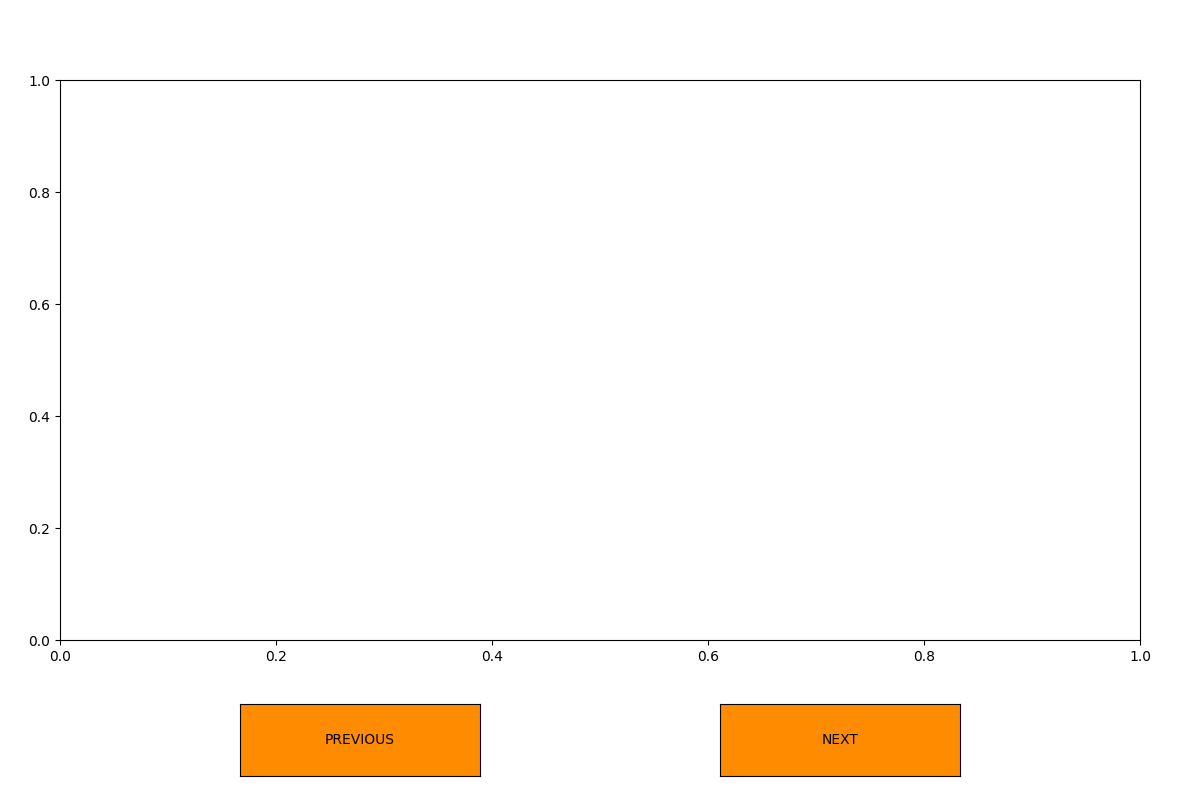
\includegraphics[width=\textwidth]{pusteokno.png}
      \caption{Puste okno wizualizacji}
    \end{figure}

    \noindent
    \quad Mamy miejsce w ramce, gdzie będą rysowane figury, linie, punkty i tp. I mamy dwa przyciski 'NEXT' i 'PREVIOUS'. 'NEXT' przełącza na następną scenę, 'PREVIOUS' na poprzednią. W zależności od wersji \textbf{matplotlib} z dołu lub z góry jest podstawowa panel sterowania z możliwością przybliżania, przesuwania i tp.

    \noindent
    \quad Omówimy niżej wszystkie operacje, które są wizualizowane przez nasze drzewa. A mianowicie wszystkie operacje przedstawione w dokumentacji, składające \textbf{API} drzew, są wizualizowane. Mają niektóre wspólne cechy:

    \begin{itemize}
        \item Wszystkie linie stanowiące podziały w drzewach są różowe (color='magenta', linewidth=2)
        \item Wszystkie punkty wrzucone do drzewa są zielone (color='green')
        \item Każdy aktualnie rozpatrywany obszar jest wydzielony szarym prostokątem (color='silver', alpha=0.4)
        \item Aktualnie rozpatrywana linia podziału jest pomarańczową (color='darkorange', linewidth=2)
    \end{itemize}

    \noindent
    \quad Na następnej stronie na rysunku 2 przedstawiona scena z wizualizacji zawierająca te wszystkie elementy:

    \newpage
    \begin{figure}[h!]
    \centering
      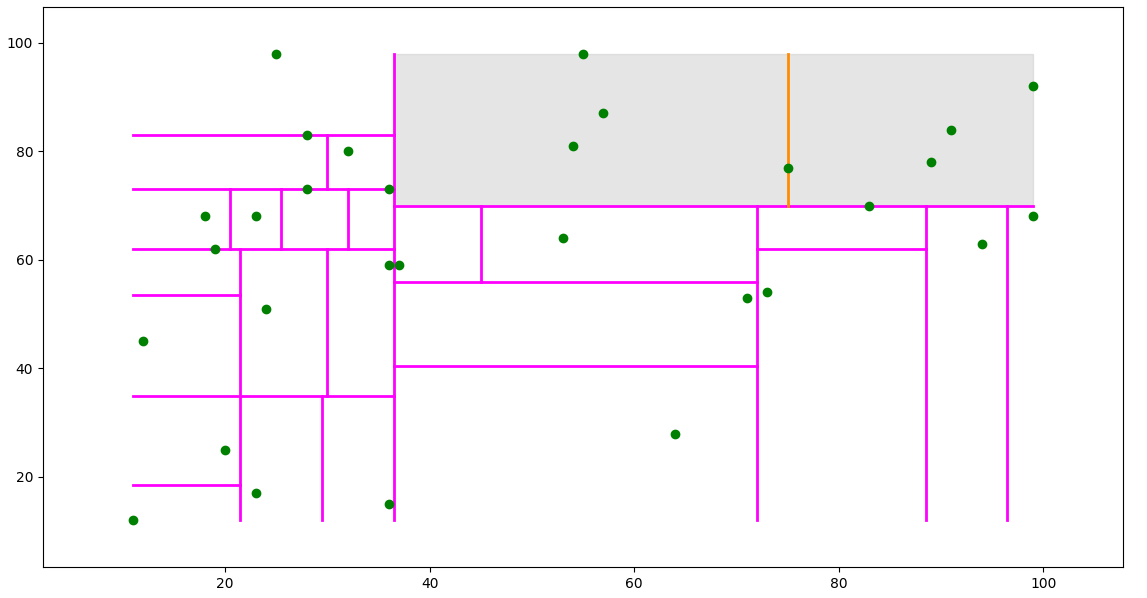
\includegraphics[width=\textwidth]{podstawowe_elementy_wiz.png}
      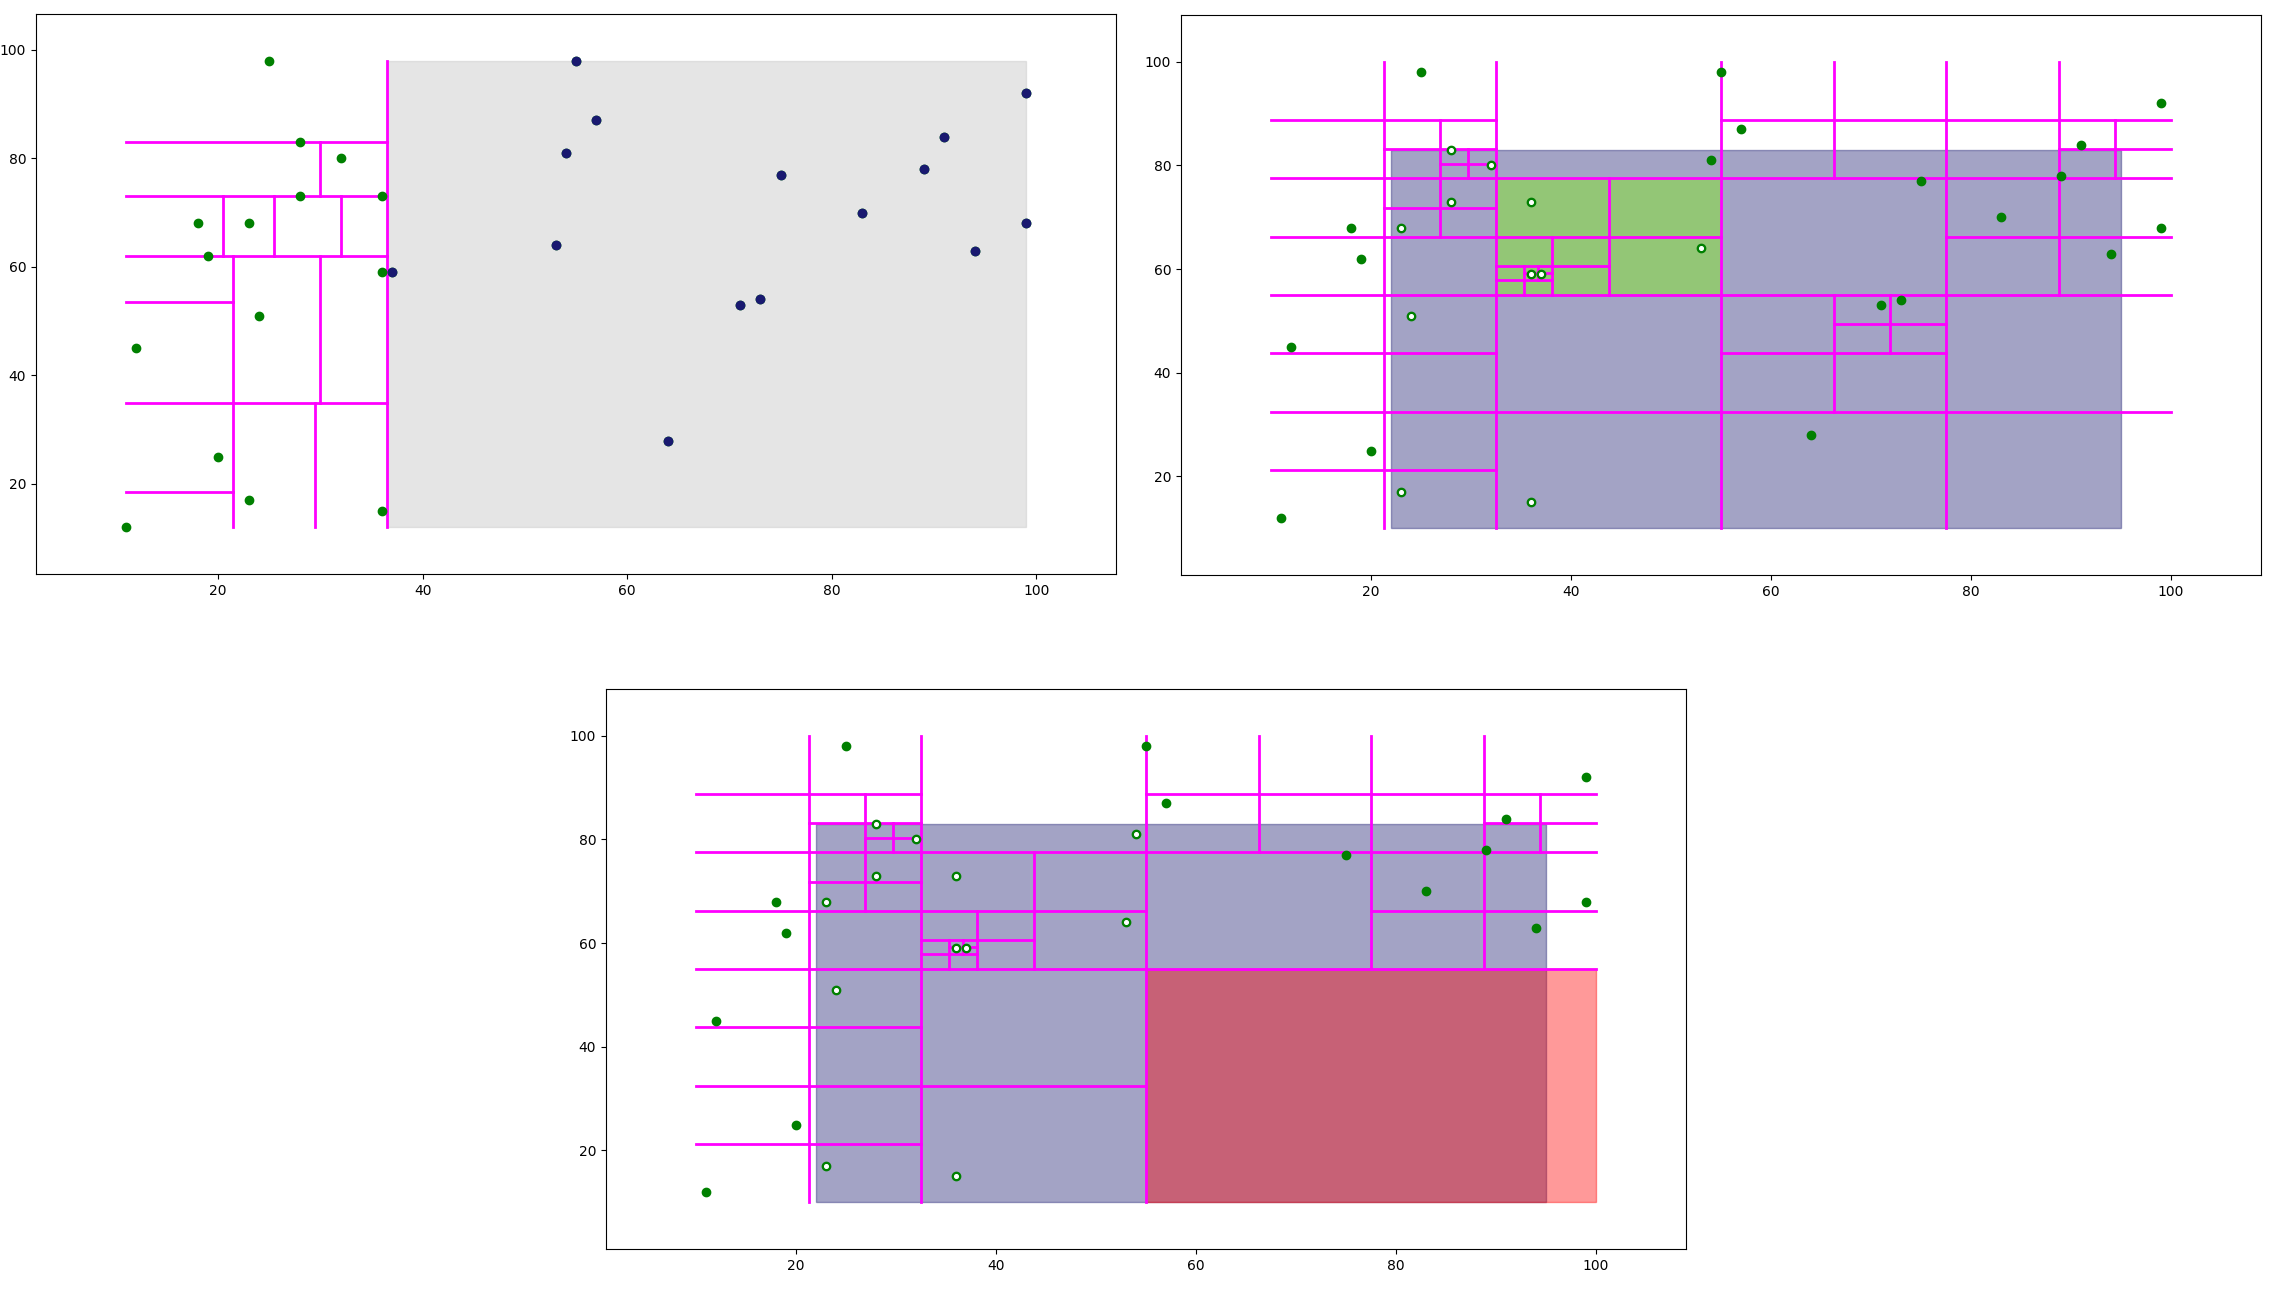
\includegraphics[width=\textwidth]{podstawowe_elementy2_wiz.png}
      \caption{Podstawowe elementy wizualizacji}
    \end{figure}

    \noindent
    \quad Jeszcze kilka podstawowych elementów:

    \begin{itemize}
        \item Aktualnie dodawany do drzewa punkt jest ciemno-niebieski (color='midnightblue')
        \item Każdy podgląd / operacja, która zakończyła się sukcesem, rysuje zielony prostokąt (color='lawngreen', alpha=0.4) (np. znaleźliśmy punkt, który musimy potem zwrócić)
        \item Każdy podgląd / operacja, która zakończyła się porażką, rysuje czerwony prostokąt (color='red, alpha=0.4) (np. spróbowaliśmy dodać tu nowy punkt, ale okazało się, że ten punkt nie należy do tego obszaru)
    \end{itemize}

    \newpage
    \subsection{KDTree}
      \subsubsection{Budowanie}
        \quad Wszystko wygląda następująco: widzimy szary prostokąt, który wydziela aktualnie rozpatrywany obszar, i widzimy ciemno-niebieskie punkty, w tym momencie próbujemy optymalnie podzielić ten obszar.

        \noindent
        \quad W następnym kroku pojawia się pomarańczowa linia podziału. Nasz szary prostokąt jeszcze pokazuje cały ten obszar, który podzieliliśmy.

        \noindent
        \quad W następnej scenie już patrzymy na jeden z dwóch otrzymanych obszarów. Nowa linia jest już pokazywana jak wszystkie na różowo. Wszystko jest jak w pierwszym kroku: tak kontynuujemy aż do końca.

        \begin{figure}[h!]
        \centering
          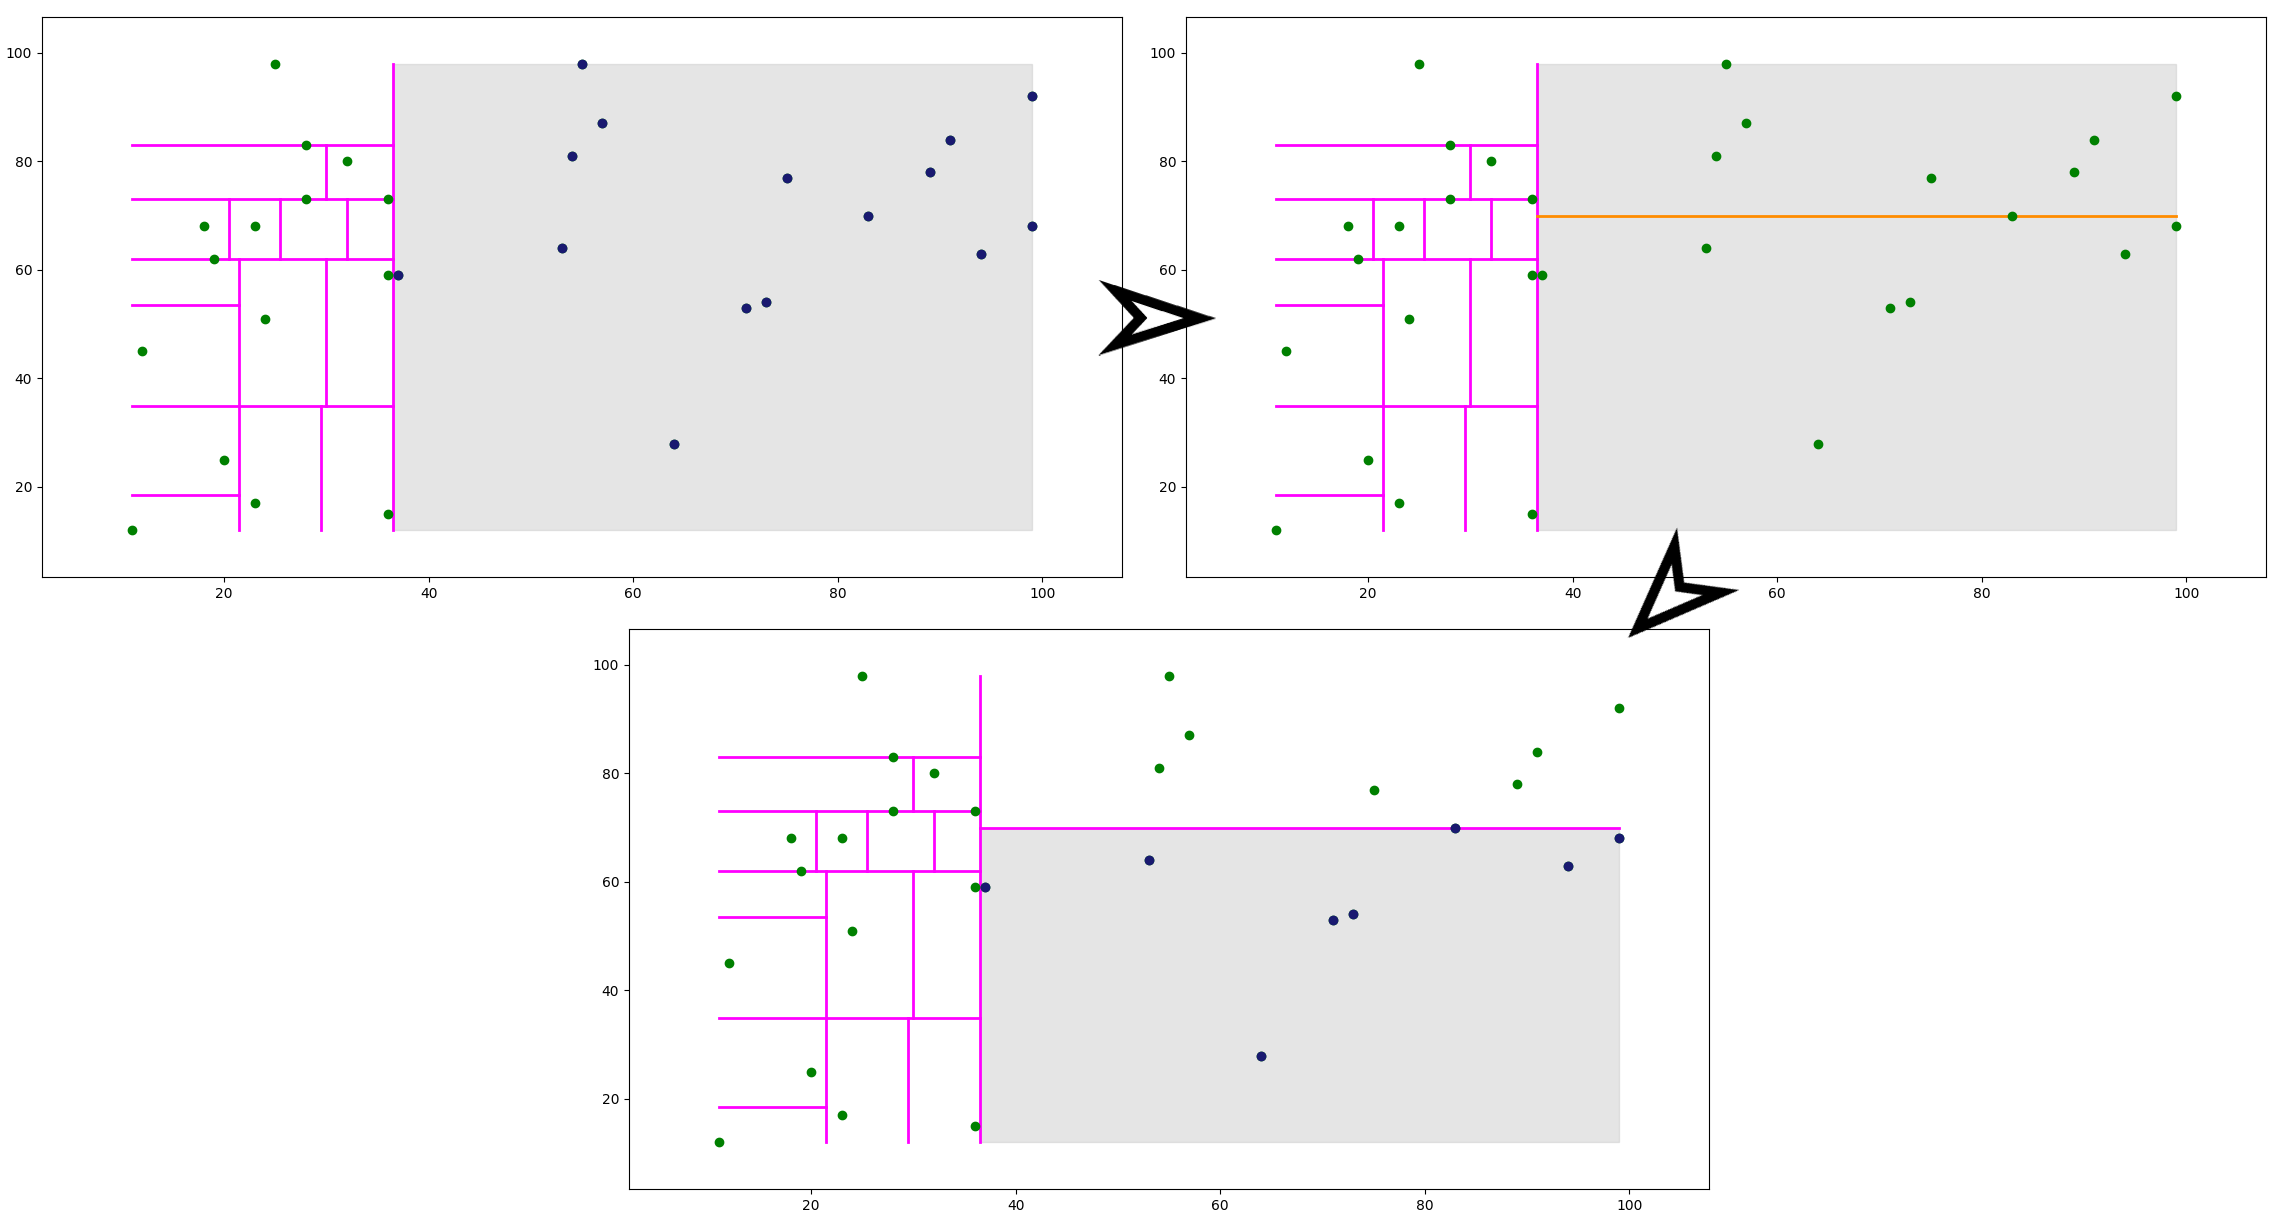
\includegraphics[width=\textwidth]{kdtree_budowanie.png}
          \caption{Wizualizacja budowania KDTree}
        \end{figure}

      \subsubsection{Sprawdzenie czy istnieje punkt}
        \begin{figure}[h!]
        \centering
          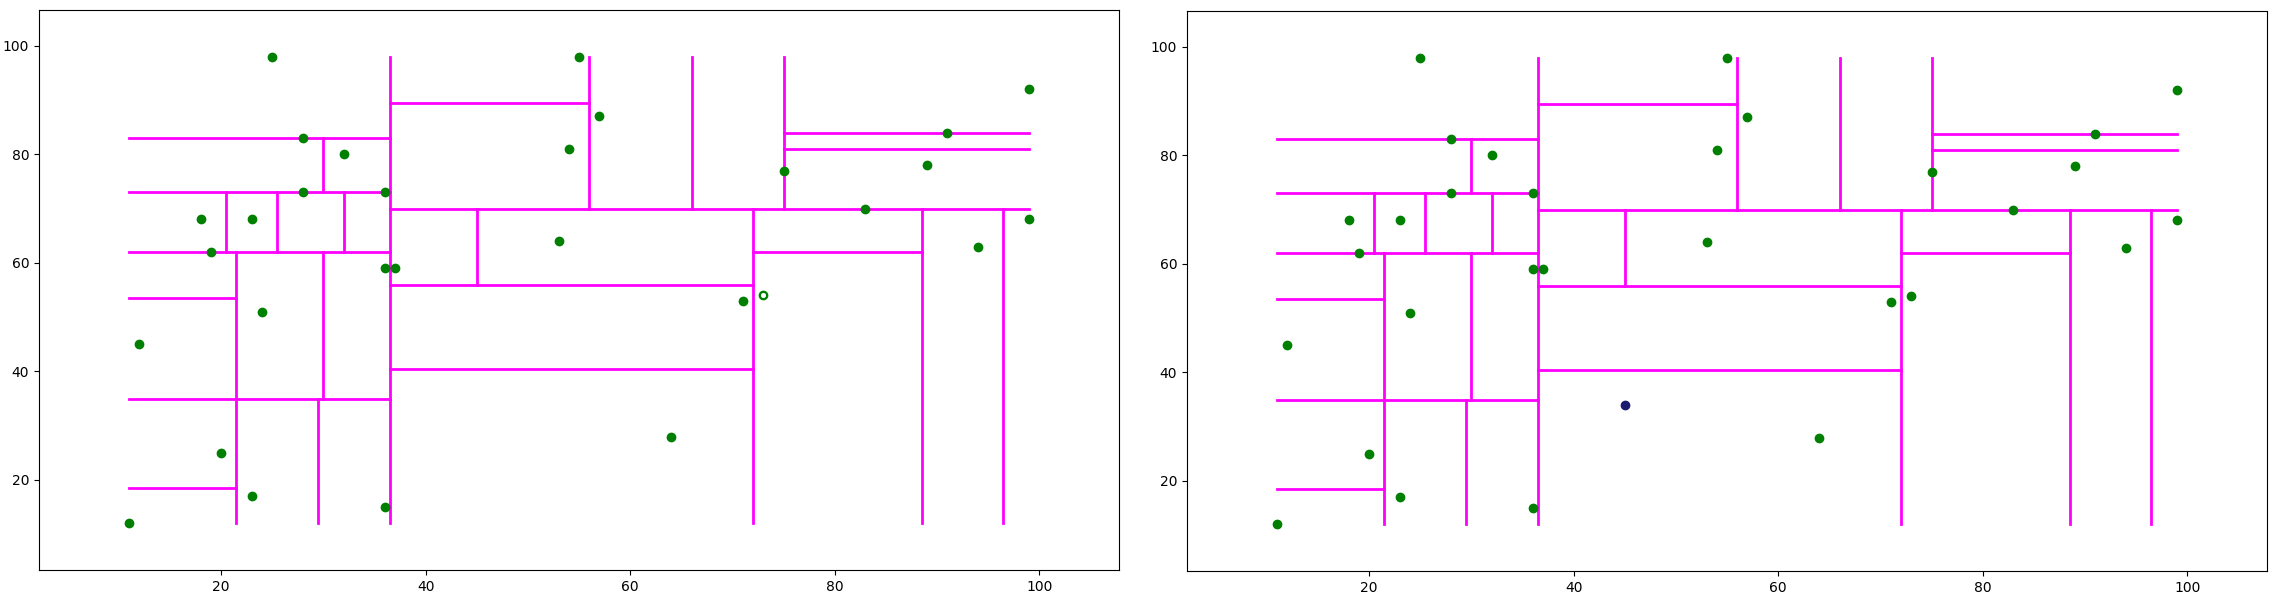
\includegraphics[width=\textwidth]{kdtree_contains_marks.png}
          \caption{Wizualizacja sprawdzenia istnienia elementu KDTree}
        \end{figure}

        \newpage

        \noindent
        \quad Na rysunku 4 zostały przedstawione 2 sytuacje. Na lewej częsci widzimy jeden punkt z pustym środkiem. W tym przypadku sprawdzamy czy istnieje ten punkt i już możemy od razu zobaczyć, że taki jest. Jest to zrobione, żeby nie było kolizji z punktami już istniejącymi, i przy tym było widać czego szukamy.
        Po prawej stronie jest już przypadek, gdy tego punktu nie istnieje, więc możemy spokojnie sobie go zaznaczyć ciemno-niebieskim kolorem.

        \noindent
        \quad W każdym kolejnym kroku schodzimy na jeden poziom głębiej, aż w końcu (gdy dojdziemy do liścia) dostajemy lub nie dostajemy szukanego punktu. Także w każdym kroku widać obszar w którym sprawdzamy i pomarańczową linię według której porównujemy.

        \begin{figure}[h!]
        \centering
          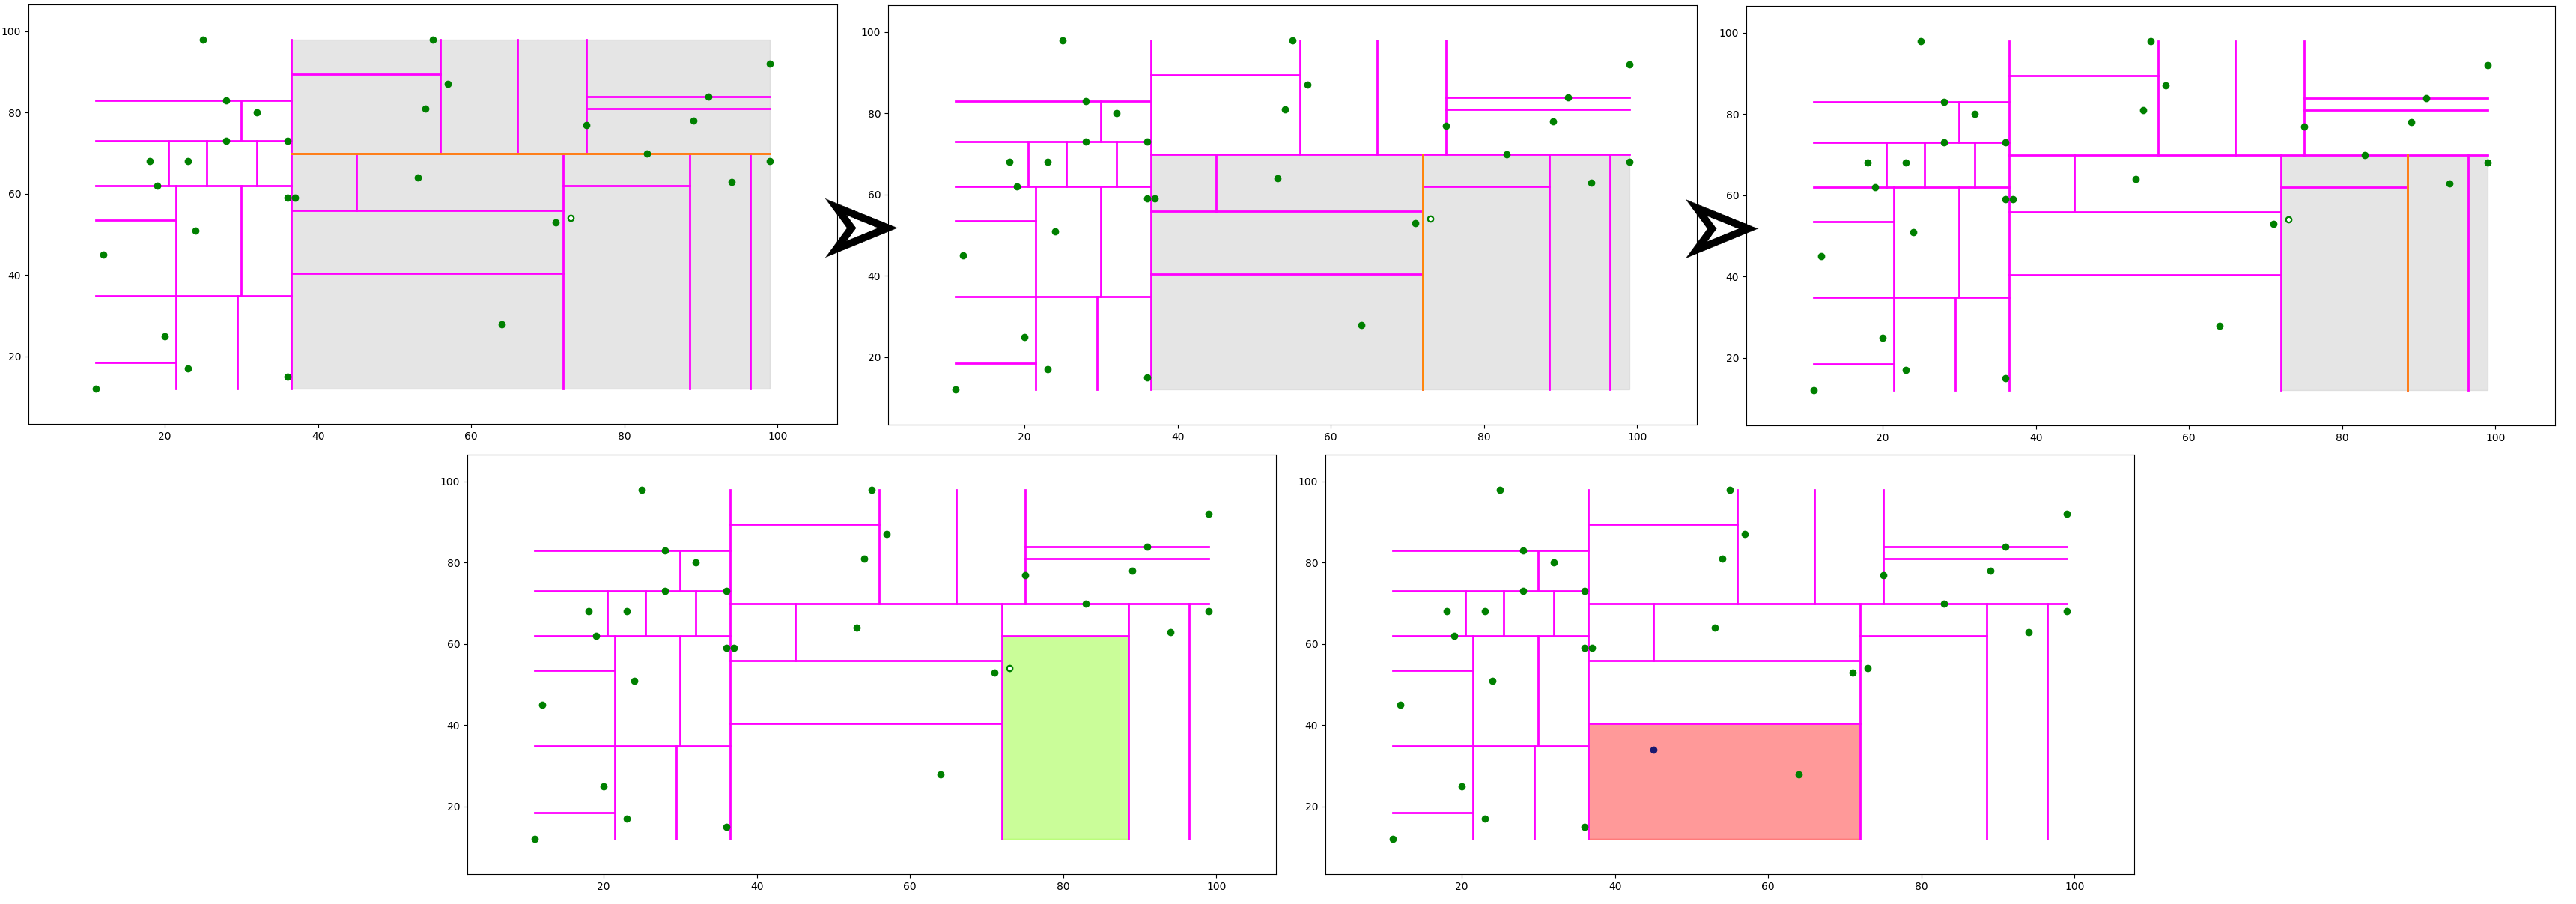
\includegraphics[width=\textwidth]{kdtree_contains.png}
          \caption{Wizualizacja kroków sprawzenia istnienia elementu KDTree}
        \end{figure}

      \subsubsection{Szukanie punktów w prostokącie}
        \quad O ile szukamy punktu w pewnym przekazanym prostokącie, to od razu sobie oznaczamy go ciemno-niebieskim kolorem. Można go zobaczyć po obu stronach na rysunku 6 niżej. Dodatkowo oznaczamy znalezione punkty (te, które znajdą się w końcowej liście) z pustym środkiem. Przykładowe oznaczenie jest po prawej stronie rysunku 6.

        \begin{figure}[h!]
        \centering
          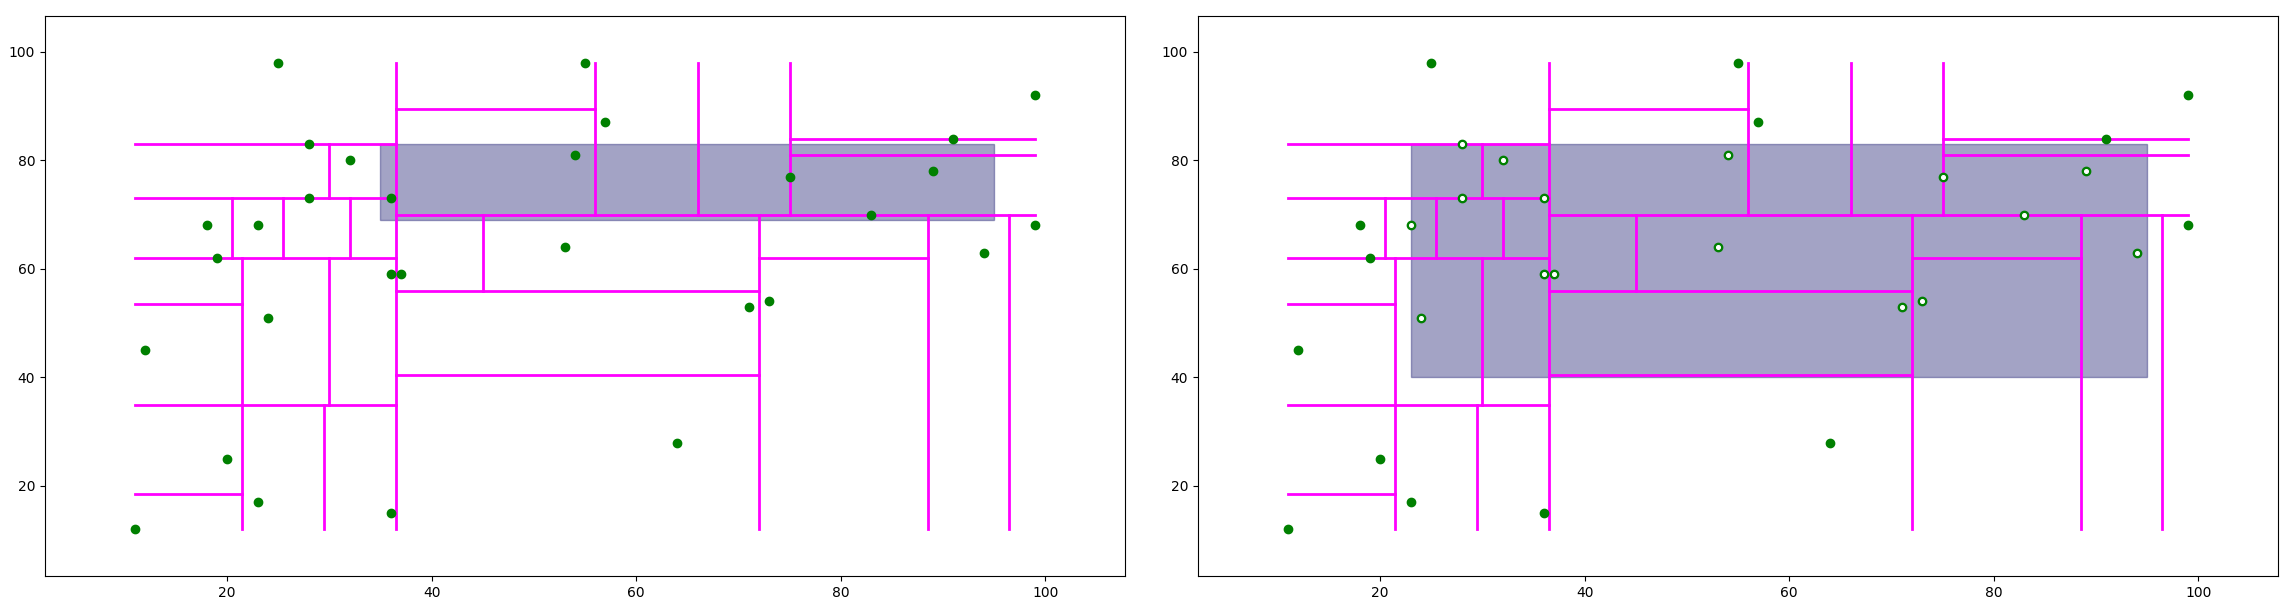
\includegraphics[width=\textwidth]{kdtree_search_marks.png}
          \caption{Wizualizacja elementów szukania punktów w prostokącie KDTree}
        \end{figure}

        \noindent
        \quad Na następnej stronie na rysunku 7 zostały przedstawione kolejne kroki wizualizacji, a także przykład wyglądu znalezienia punktów i porażki w ich szukaniu dla pewnego obszaru.

        \newpage

        \begin{figure}[h!]
        \centering
          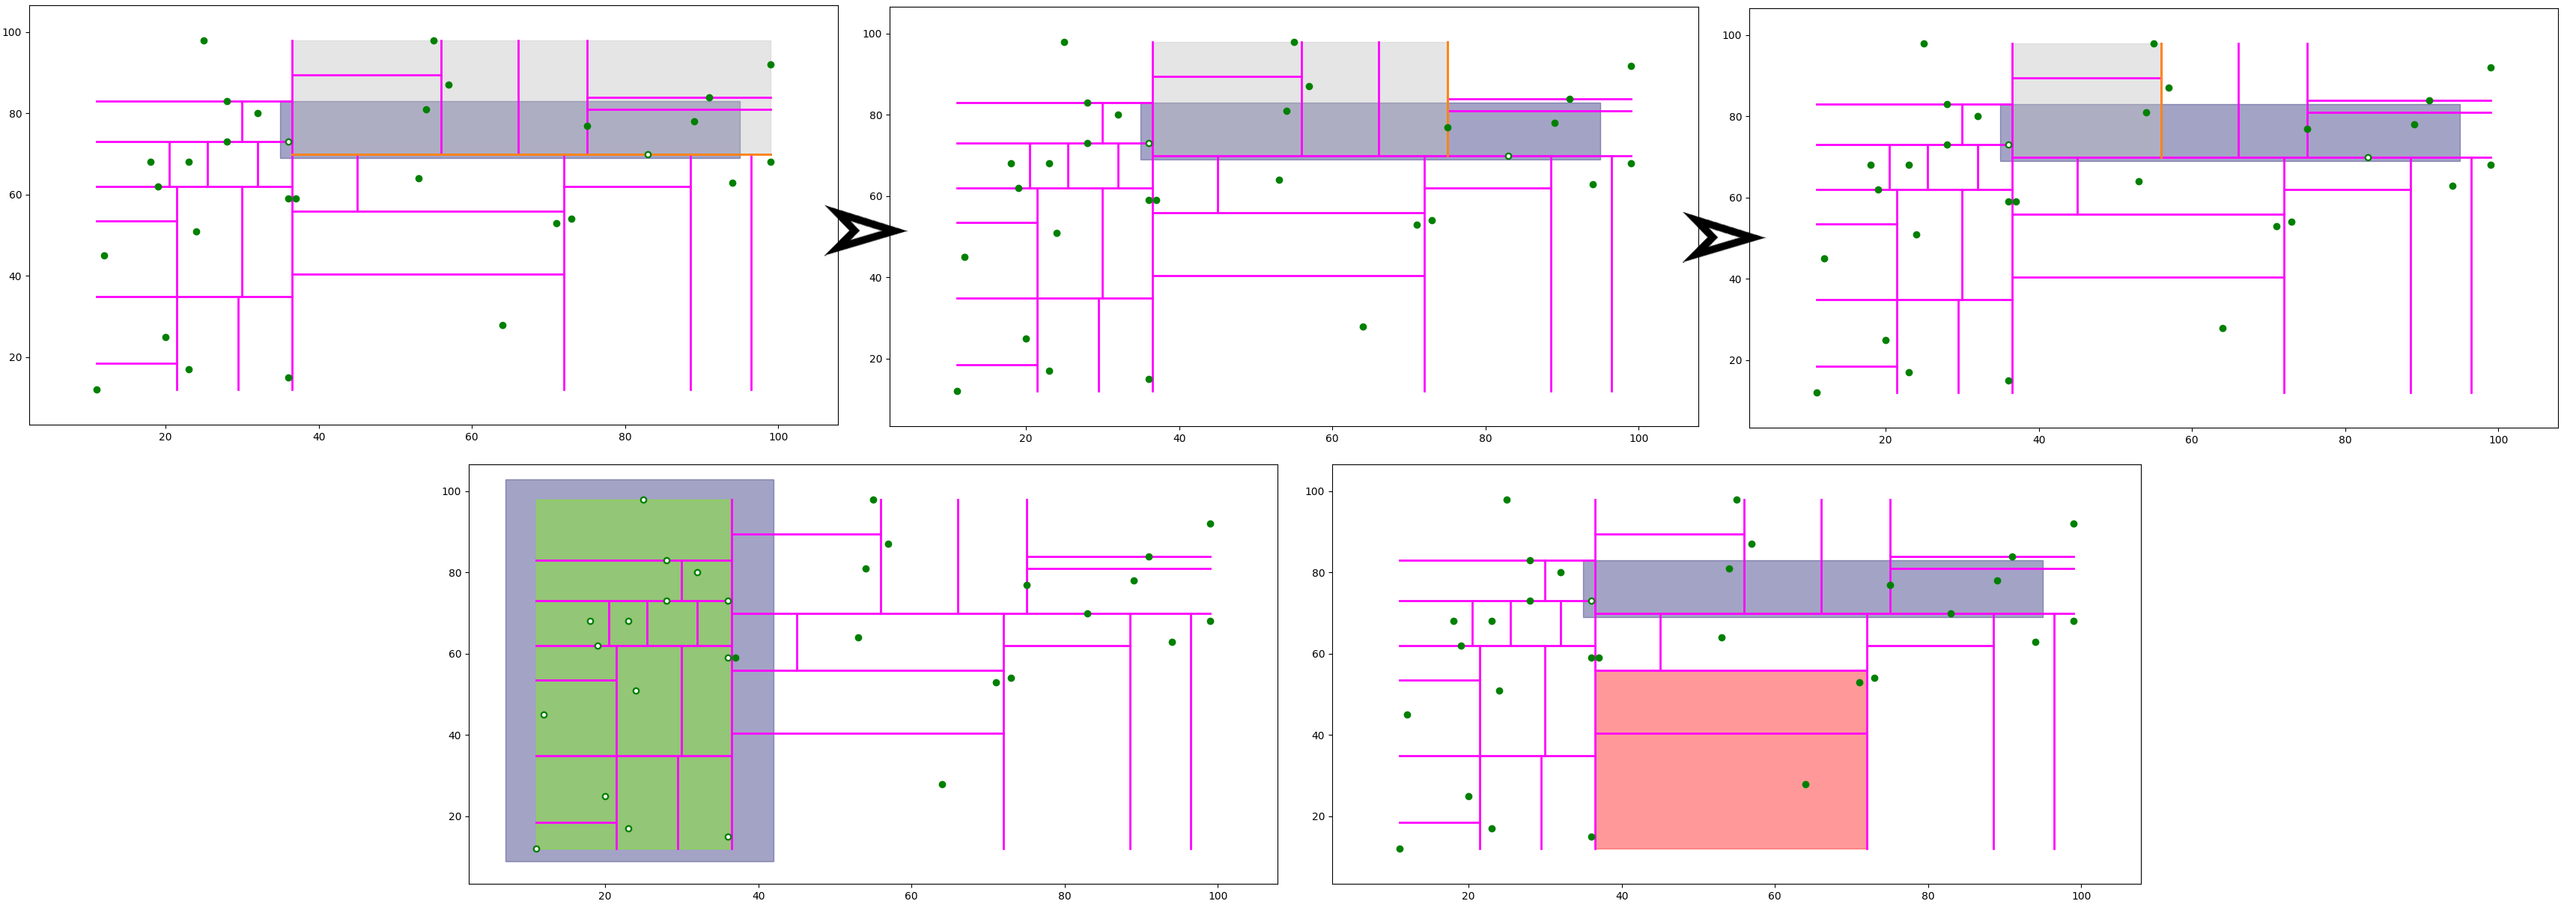
\includegraphics[width=\textwidth]{kdtree_search.png}
          \caption{Wizualizacja kroków szukania punktów w prostokącie KDTree}
        \end{figure}

        \noindent
        \quad W każdym kroku pokazujemy pomarańczową linię według której poszliśmy w jedną ze stron i odpowiednio szarym prostokątem pewien obszar. Robimy to do tej pory póki ten obszar ma część wspólną z prostokątem szukanym. Jeżeli nie ma, to jest on pokazywany czerwonym. Jeżeli całkiem zawiera się, lub jest liściem i znaleźliśmy punkt, który należy do szukanego prostokąta, to rysujemy na zielono jak na rysunku 7.

    \subsection{QuadTree}
      \subsubsection{Budowanie / Wstawianie punktów}
        \quad Te dwie rzeczy są połączone dlatego, że budowanie korzysta ze wstawiania punktów, więc jest sens, żeby były przedstawione razem.

        \noindent
        \quad Wizualizacja tego jest dość skomplikowana, czego nie da się powiedzieć o algorytmie. Niżej na rysunku 8 zostało przedstawiono 9 kolejnych kroków wizualizacji.

        \begin{figure}[h!]
        \centering
          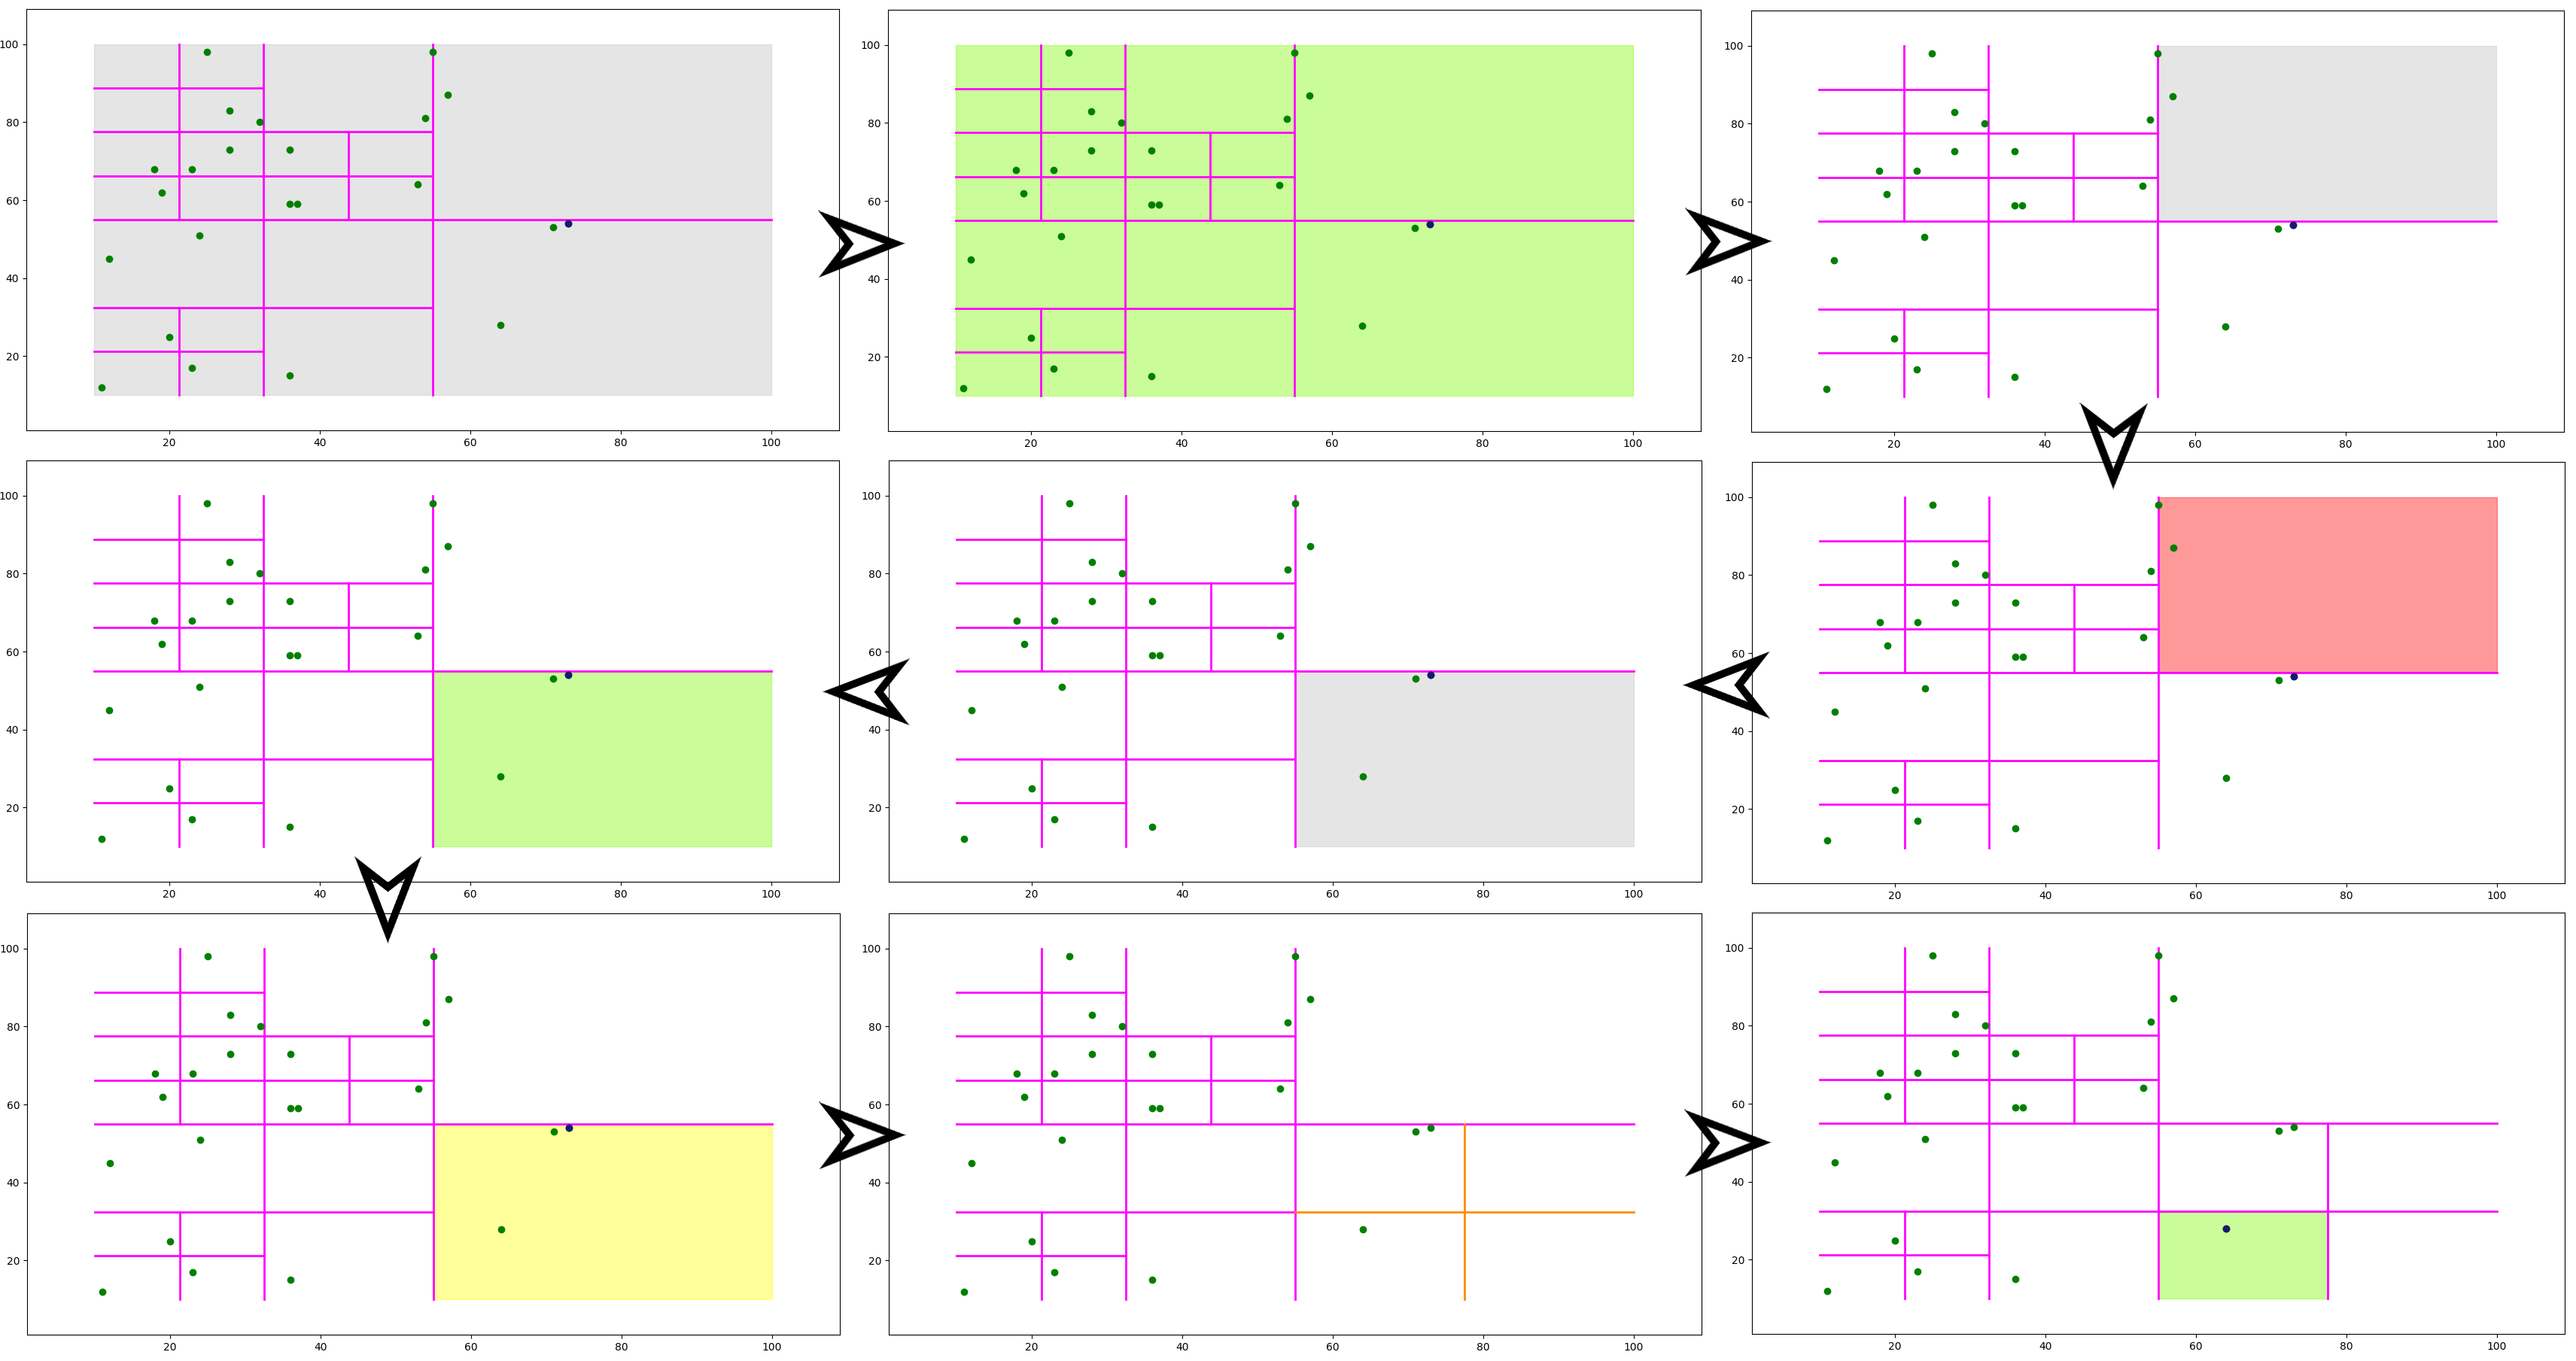
\includegraphics[width=\textwidth]{quad_build.png}
          \caption{Wizualizacja kroków budowania QuadTree}
        \end{figure}

        \noindent
        \quad Otóż, algorytm polega na tym, że jak jesteśmy na pewnym poziomie głębokości i chcemy wstawić jakiś punkt (w tym przypadku ciemno-niebieski), to sprawdzamy kolejne ćwiartki dopóki nie znajdziemy potrzebną (zaświeci się zielonym kolorem). Idziemy poziom niżej. Jak dojdziemy do liścia, to ostatecznie dodajemy nasz punkt (zaświeci się zielonym). Ale może zdarzyć się, że przepełnimy liść i trzeba będzie go podzielić. Wtedy on zaświeci się żółtym, a w następnym kroku pojawią się pomarańczowe linie dzielące ten liść. Dalej wszystkie punkty w tym liściu, w tym i nasz nowy, będą wstawiane do nowych liści podobnym sposobem jak i nowy punkt (próbując wstawić do każdego liścia i dostając czerwony lub zielony kolor jako oznaczenie porażki i sukcesu odpowiednio).

      \subsubsection{Szukanie punktów w prostokącie}
        \quad Wizualizacja tej operacji jest bardzo podobna do wizualizacji w drzewie KDTree. Sprawdzamy kolejne ćwiartki drzewa, i jeżeli obszar przecina się z szukanym prostokątem, to idziemy wgłąb. Jeżeli obszar całkiem zawiera się w prostokącie lub pewne punkty liścia należą do szukanego prostokąta, to ten obszar świeci się zielonym. Jeżeli obszar nie przecina się z szukanym, lub jest pustym, lub żaden punkt nie należy do szukanego, to zaświeci się na czerwono. Przykładowo jest pokazane na rysunku 9 niżej.

        \begin{figure}[h!]
        \centering
          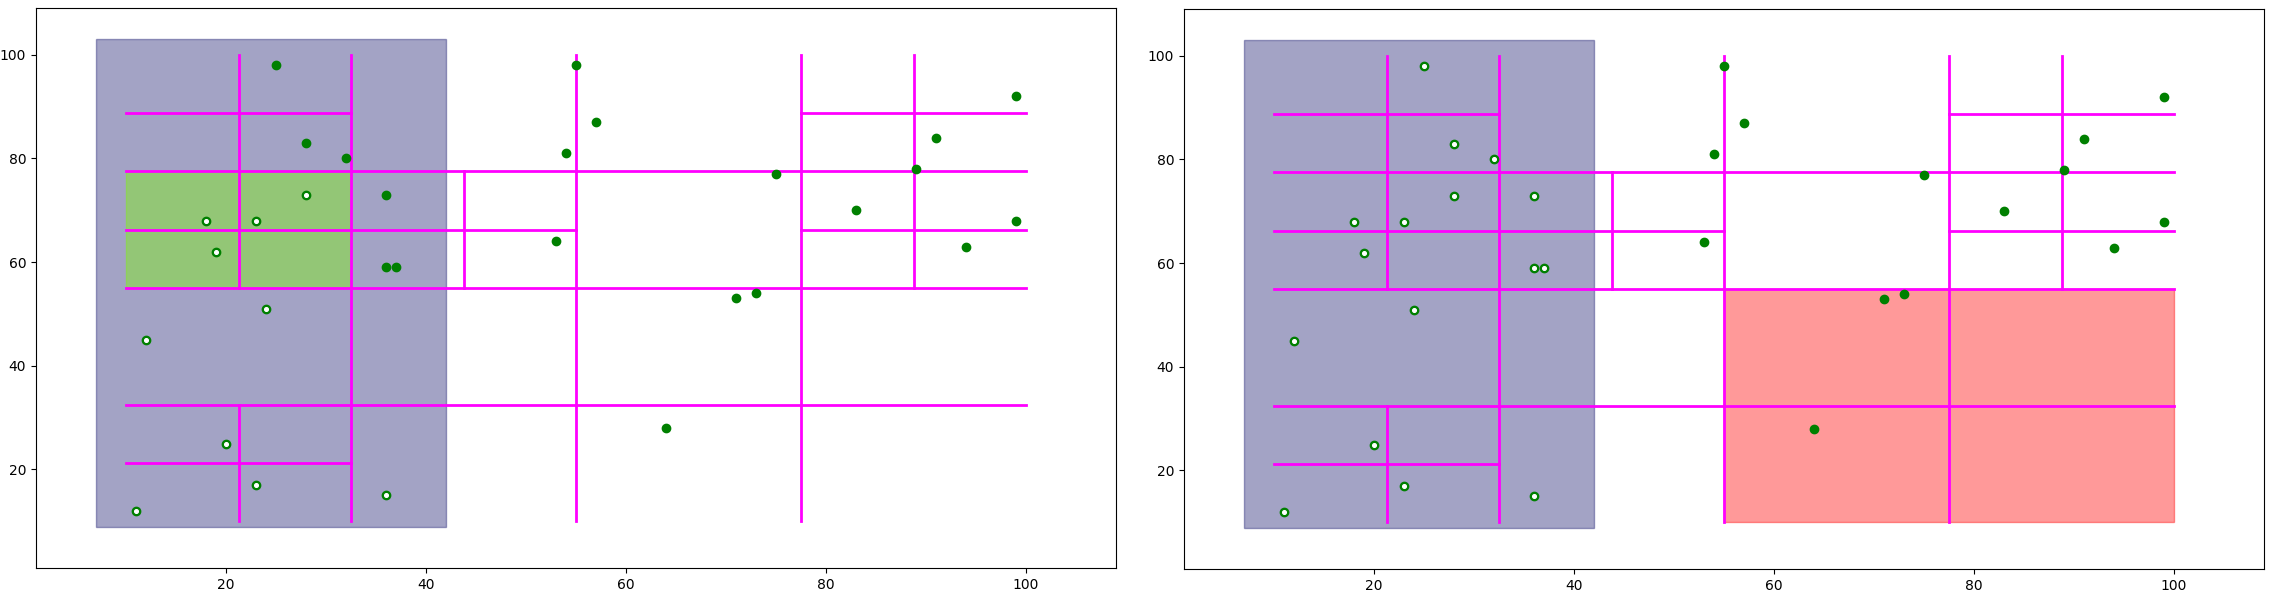
\includegraphics[width=\textwidth]{quad_search.png}
          \caption{Wizualizacja kroków szukania punktów w prostokącie QuadTree}
        \end{figure}

  \section{Dodatkowe uwagi}
    \subsection{Przepełnienie stosu}
      \quad Czasami dla bardzo dużych zbiorów danych i przy pewnych bug'ach, które zostały już naprawione (wciąż mogą istnieć podobne, jeszcze nie wykryte), przepełniał się stos. Jest dwie możliwości: mamy nieskończoną rekurencję lub rekurencja jest skończona, ale bardzo głęboka. Najprostszym sposobem jest użycie modułu \textbf{sys} i \textbf{inspect}. Sprawdzić i ustawić aktualną maksymalną głębokość stosu da się następująco:
      \begin{python}
      >>> import sys
      >>> sys.getrecursionlimit()
      1000
      >>> sys.setrecursionlimit(7500)
      >>> sys.getrecursionlimit()
      7500
      \end{python}

      \noindent
      \quad Żeby monitorować aktualną głębokość stosu, w funkcji rekurencyjnej warto użyć funkcji z modułu \textbf{inspect}.
      \begin{python}
      >>> import inspect
      >>> len(inspect.stack(0))
      1  # 1 because we are calling from main
      >>> def check_stack():
      ...     print(len(inspect.stack(0)))
      ...
      >>> check_stack()
      2  # we are 1 more level deeper (called inside check_stack() function)
      \end{python}

      \noindent
      \quad Dla \textbf{QuadTree} przy obecności bardzo dużego punktu (współrzędne rzędu $10^{20}$ i dwóch o bardzo małej odległości między sobą rzędu $10^{-15}$, dostajemy maksymalną głębokość stosu równą 127. Czyli jest bardzo mała szansa wygenerowania danych, które by ten stos podstawowy przepełniły, ale wciąż szansa istnieje.

    \subsection{Przepełnienie pamięci}
      \quad Jeszcze jednym problemem może okazać się przepełnienie pamięci operacyjnej, co powoduje \textbf{MemoryError}. Jest to zazwyczaj przy włączonej wizualizacji dla bardzo dużych zbiorów danych i jest największa szansa przy konstruowaniu \textbf{QuadTree}, ponieważ dla niego wizualizacja zawiera bardzo dużo kroków. Dla 10000 punktów przy włączonej wizualizacji jeden tylko rysunek \textbf{KDTree} zajmował ponad 6gb RAM. Więc warto zauważyć, że nie trzeba włączać wizualizację dla bardzo dużych zbiorów. Dla \textbf{QuadTree} rysunek zajmował ponad 10gb RAM po czym wyskoczyła \textbf{MemoryErro}. Rysunek tak i nie został wyświetlony.

    \subsection{Duże zbiory a wizualizacja}
      \quad Jeszcze jednym argumentem, żeby nie włączać wizualizację dla dużych zbiorów jest niemożliwość odczytanie czegokolwiek z tej wizualizacji i długość przełączania scen. Jedyną możliwościa odczytania czegoś z scen jest przełączenia do tyłu, żeby zobaczyć końcowy wynik, i potem używania narzędzi \textbf{matplotlib}, żeby popatrzyć na pewne części bardziej szczegółowo. Wtedy da się odczytać coś z rysunku. W ogólnych sytuacjach polecamy unikać stosowania wizualizacji dla dużych zbiorów.

      \begin{figure}[h!]
      \centering
        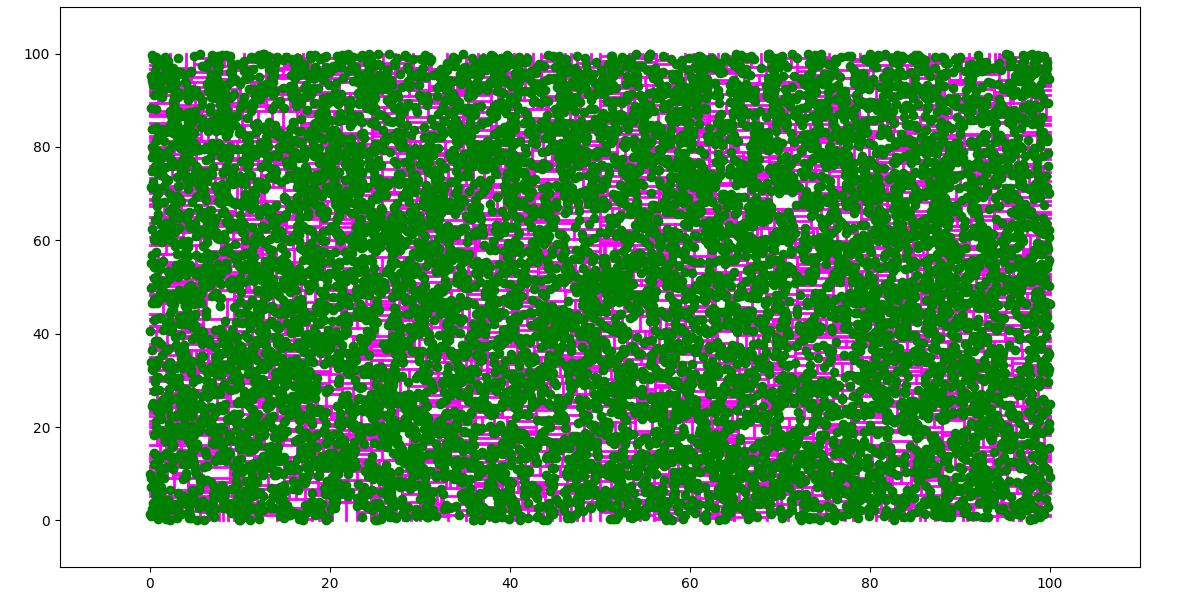
\includegraphics[width=0.9\textwidth]{kdtree_huge_lastscene.png}
        \caption{Ostatnia scena konstruowania KDTRee dla 10tys.-el. zbioru}
      \end{figure}

\newpage
\part{Sprawozdanie}
  \setcounter{section}{0}

  \section{Wstęp teoretyczny}
    \quad W wykonywanym przez nas ćwiczeniu zajęliśmy się problemem przeszukiwania zbioru punktów w celu znalezienia tych, które należą do zadanego przez nas obszaru. Przygotowaliśmy dwa rozwiązania wspomnianego problemu. Pierwszy z nich wykorzystuje strukturę QuadTree, drugi strukturę KDTree.

    \subsection{Struktura QuadTree}
      \quad Jest to struktura danych będąca drzewem, które służy do podziału przestrzeni dwuwymiarowej na mniejsze części, dzieląc ją na równe ćwiartki, a następnie dzieląc je na kolejne ćwiartki itd. W naszym problemie, naszą prostokątną płaszczyznę będziemy dzielić na ćwiartki wtedy, kiedy w danym polu znajdować się będzie więcej niż jeden punkt, tak aby na każde pole przypadł maksymalnie jeden punkt. Możliwym jest także przyjęcie pewnej maksymalnej głębokości drzewa, która będzie oznaczała maksymalną ilość podziałów, wówczas w danych polach znajdować się będzie mógł więcej niż jeden punkt, dla odmiany możemy też przyjąć konkretną ilość punktów inną niż 1, jako akceptowalną do zakończenia podziałów prostokąta.  Nasz podzielony prostokąt reprezentowany będzie przez drzewo czwórkowe. Korzeń reprezentuje główny prostokąt, a gałęzie z niego wyrastające, jego podział. Analogicznie będzie z kolejnymi podziałami prostokątów, podział prostokąta na ćwiartki reprezentują 4 gałęzie z niego wychodzące. Liście tego drzewa będą, więc prostokątami, które nie zostały podzielone. Przykładowy podział prostokąta zgodnie z powyżej opisaną koncepcją i drzewo czwórkowe mu odpowiadające, ilustruje poniższy rysunek: 

      \begin{figure}[h!]
      \centering
        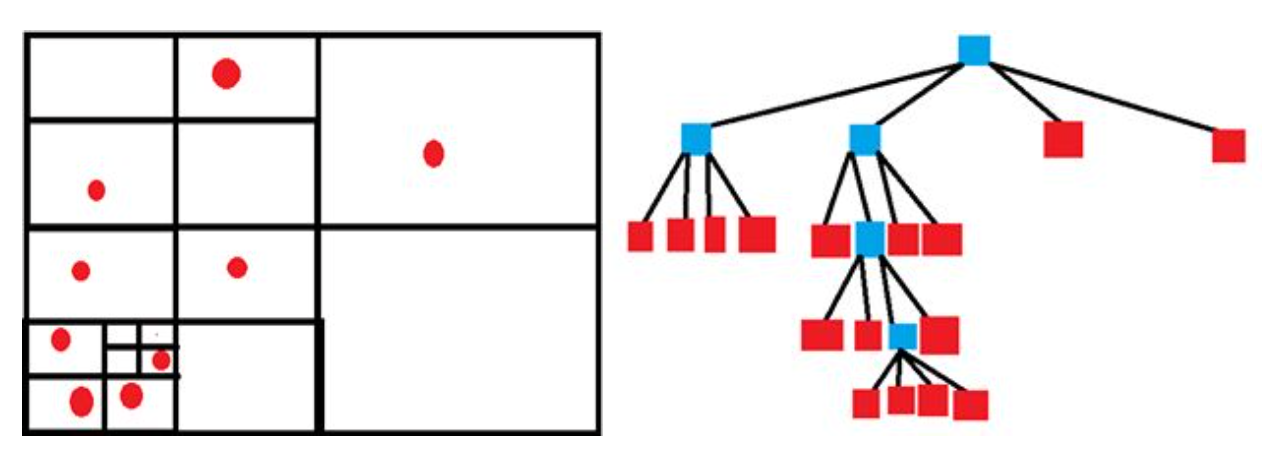
\includegraphics[width=\textwidth]{quadtree_structure.png}
        \caption{Struktura QuadTree}
      \end{figure}

      \noindent
      \quad Złożoność czasowa, jak i pamięciowa tworzenia QuadTree zależy stricte od jego głębokości (ona zależy natomiast od rozmieszczenia punktów na płaszczyźnie) oraz ilości punktów leżących na płaszczyźnie i wynosi $O((d+1)*n)$, gdzie $d$ – głębokość drzewa, $n$ – liczba punktów. Mając już odpowiednio zaimplementowane QuadTree możemy je w prosty sposób wykorzystać do rozwiązania naszego problemu – znalezienia punktów znajdujących się na podanym obszarze. Przeszukujemy nasze drzewo, zaczynając od korzenia,  natrafiając na kolejne węzły wykonujemy następujące operacje: 

      \begin{itemize}
          \item jeżeli prostokąt reprezentujący dziecko węzła zawiera się całkowicie w obszarze, w którym szukamy punktów, to wszystkie punkty należące do niego (całej gałęzi zaczynającej się od niego) zawierają się w prostokącie, więc dodajemy je do zbioru poszukiwanych punktów, i nie wchodzimy dalej w głąb gałęzi (odcinamy gałąź) 
          \item jeżeli prostokąt reprezentujący dziecko węzła wcale nie zawiera się w obszarze, w którym szukamy punktów, to wszystkie punkty należące do niego (całej gałęzi zaczynającej się od niego) nie zawierają się w prostokącie, więć gałąź przestajemy przeszukiwać (odcinamy gałąź)
          \item jeżeli prostokąt reprezentujący dziecko węzła częściowo zawiera się w obszarze, w którym szukamy punktów, to wchodzimy w głąb gałęzi, jeżeli natrafiliśmy na liść, sprawdzamy bezpośrednio czy punkty należące do tego liścia należą do przeszukiwanego obszaru, jeżeli tak to dany punkt dodajemy do zbioru poszukiwanych punktów 
      \end{itemize}

      \noindent
      \quad Złożoność obliczeniowa przeszukania takiego QuadTree wynosi $O(dl)$, gdzie $d$ - głębokość drzewa, $l$ – liczba liści reprezentujących prostokąty częściowo zawierające się w przeszukiwanym obszarze. Przeszukanie takiego drzewa jest, więc w praktyce znacząco mniej kosztowne niż jego stworzenie. Struktura ta w zależności od sytuacji i zbioru punktów może okazać się bardzo optymalna, a także wręcz przeciwnie, może okazać się gorsza niż przeszukiwanie poprzez sprawdzanie każdego punktu osobno. Należy, więc korzystać z niej rozważnie i dla właściwych zbiorów punktów. Tym jakie zbiory są odpowiednie, a jakie nie, zajmiemy się w dalszej części sprawozdania testując już zaimplementowany przez nas algorytm. 

    \subsection{Struktura KDTree}
      \quad Jest to struktura danych będąca drzewem binarnym, używana do podziału przestrzeni. Podana przestrzeń $k$ wymiarowa będzie tworzona w następujący sposób (równolegle przedstawione będzie tworzenie KDTree). Wśród punktów należących do przestrzeni wybieramy medianę przy pomocy QuickSelect, jest ona punktem podziału. Należy przed tym wybrać wymiar podziału, możemy dokonywać wyboru na dwa sposoby, na przemian lub wybierając ten gdzie różnica współrzędnych punktów jest największa. My w swojej implementacji wybraliśmy ten drugi, gdyż pozwala on uzyskać lepszą strukturę drzewa. Gdy dokonujemy danego podziału wówczas nasza obecna przestrzeń zostanie podzielona na dwie części. Odpowiada to utworzeniu dwóch nowych gałęzi z węzła, który reprezentuje właśnie podzieloną przestrzeń. W węźle posiadającym gałęzie przechowujemy informacje o wymiarze podziału przestrzeni, którą został on podzielony.  Podziału przestrzeni dokonujemy wtedy, gdy dana przestrzeń zawiera więcej niż jeden punkt. Gdy zawiera dokładnie jeden, umieszczamy go jako liść naszego drzewa, wychodzący z węzła reprezentującego przestrzeń, której bezpośrednią podprzestrzenią jest ta, w której znajduje się omawiany punkt. Opisany powyżej schemat postępowania dla przykładowego zbioru punktów dwuwymiarowych ilustruje poniższy rysunek (wybór podziału przestrzeni metodą na przemian): 

      \newpage
      \begin{figure}[h!]
      \centering
        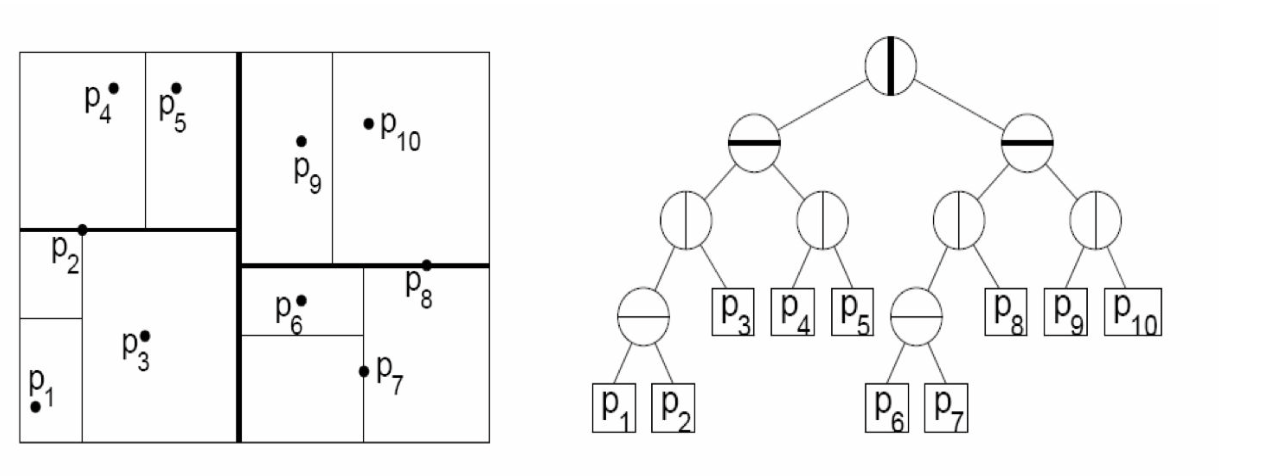
\includegraphics[width=\textwidth]{kdtree_structure.png}
        \caption{Struktura KDTree}
      \end{figure}

      \noindent
      \quad Złożoność obliczeniowa tworzenia KDTree wynosi $O(knlogn)$, dla pewnych implementacji $O(nlogn)$, gdzie $n$ to ilość punktów, a $k$ - ilość wymiarów, wynika ona bezpośrednio z głebokości drzewa, która wynosi $logn$, jeżeli zakładamy, że drzewo jest zbalansowane, a takie właśnie tworzymy.  Algorytm poszukiwania punktów należących do konkretnego obszaru jest niemal identyczny jak ten przy wykorzystaniu quadtree. Wykorzystujemy natomiast do tego strukturę KDTree co wpływa na poprawę złożoności dla niektórych przypadków. Dla drzewa zrównoważonego złożoność czasowa zliczania wynosi $O(\sqrt{n})$, złożoność czasowa wyszukiwania $O(\sqrt{n} + k)$, gdzie $k$ - jest ilością punktów wynikowych, a złożoność pamięciowa $O(n)$. Widać, więc że tak jak i w quadtree, przeszukiwanie drzewa jest znacząco mniej kosztowne niż jego stworzenie. Porównywaniem QuadTree oraz KDTree zajmiemy się w dalszej części sprawozdania na podstawie konkretnych przykładów, dzięki którym będziemy mogli dostrzec wady i zalety, a także podobieństwa i różnice tych dwóch podejść rozwiązujących problem zaklasyfikowania punktów z danego zbioru do konkretnego obszaru.


  \section{Testowanie dla różnych danych wejściowych}
    \quad Przygotowaliśmy dużo zbiorów testowych, mających na celu ustalić poprawność działania zaimplementowanych struktur oraz metod poszukujących punktów należących do danego prostokąta. Porównamy także czas działania tych metod oraz samej inicjalizacji struktur. 

    \subsection{Zbiór o rozkładzie jednostajnym}
      \quad Jest to zbiór losowo wybranych punktów należących do danego prostokąta. Natomiast obszar, w którym mamy odnaleźć punkty to prostokąt częściowo przecinający nasz zbiór punktów. W związku z losowym położeniem punktów na płaszczyźnie są one na niej równomiernie rozłożone, jest to więc przypadek dość powszechny, pozbawiony ekscesów. Dlatego został on wybrany przez nas jako pierwszy zbiór do przeanalizowania, aby sprawdzić działanie programów dla tak podstawowego zbioru punktów. 

      \noindent
      \quad Poniższe ilustracje demonstrują wyniki działania programów dla 1000 punktów:

      \newpage
      \begin{figure}[h!]
      \centering
        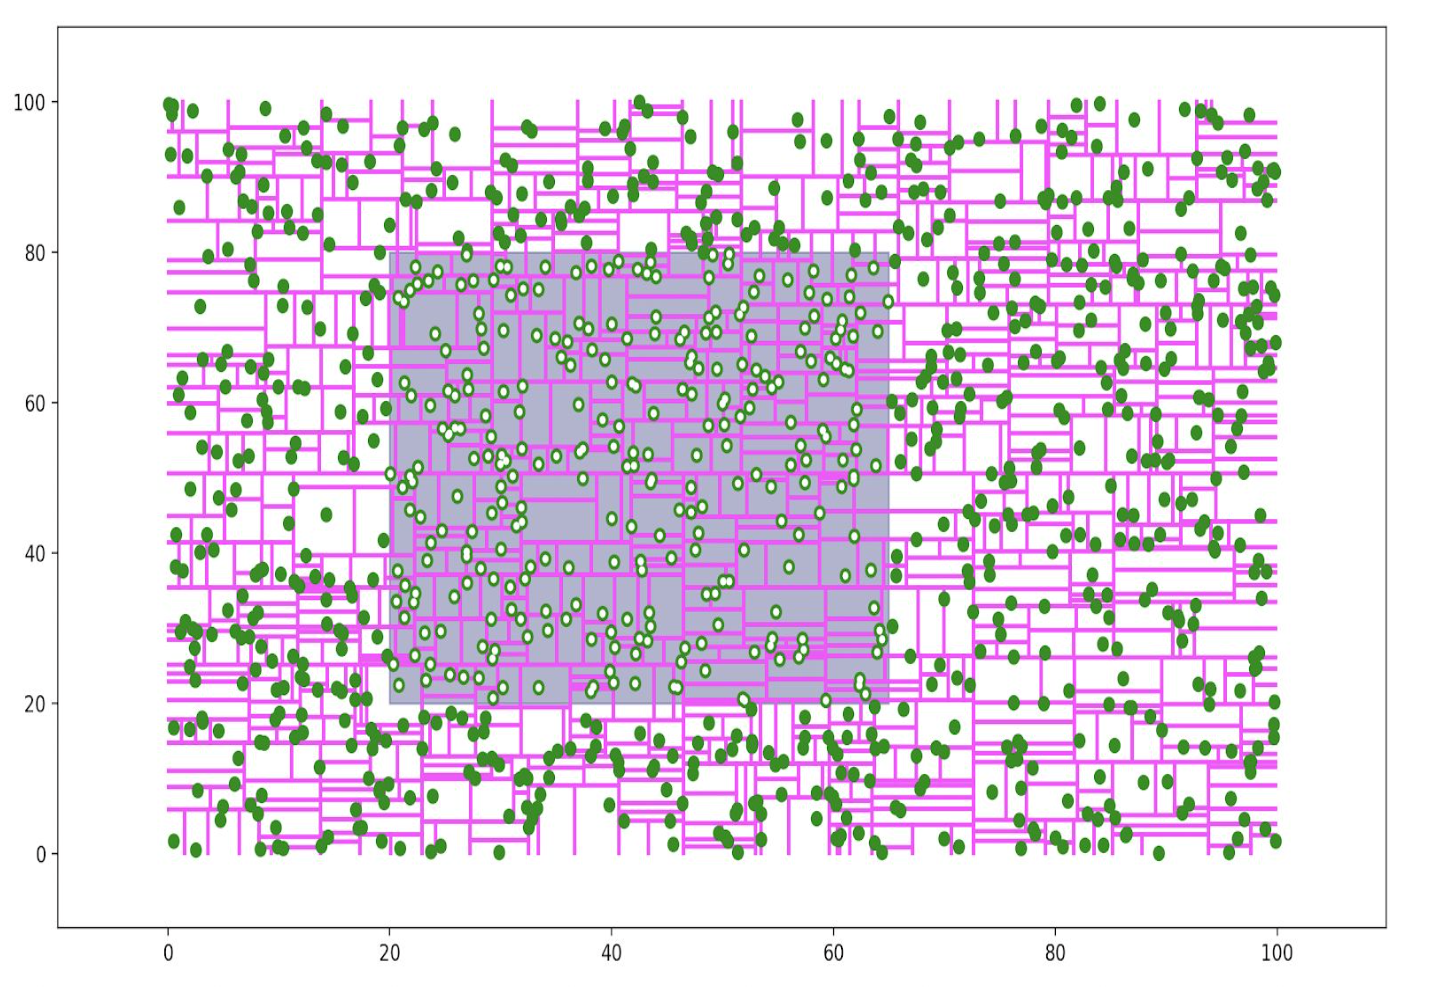
\includegraphics[width=0.9\textwidth]{krandom.png}
        \caption{Zbiór o rozkładzie jednostajnym KDTree}
      \end{figure}

      \begin{figure}[h!]
      \centering
        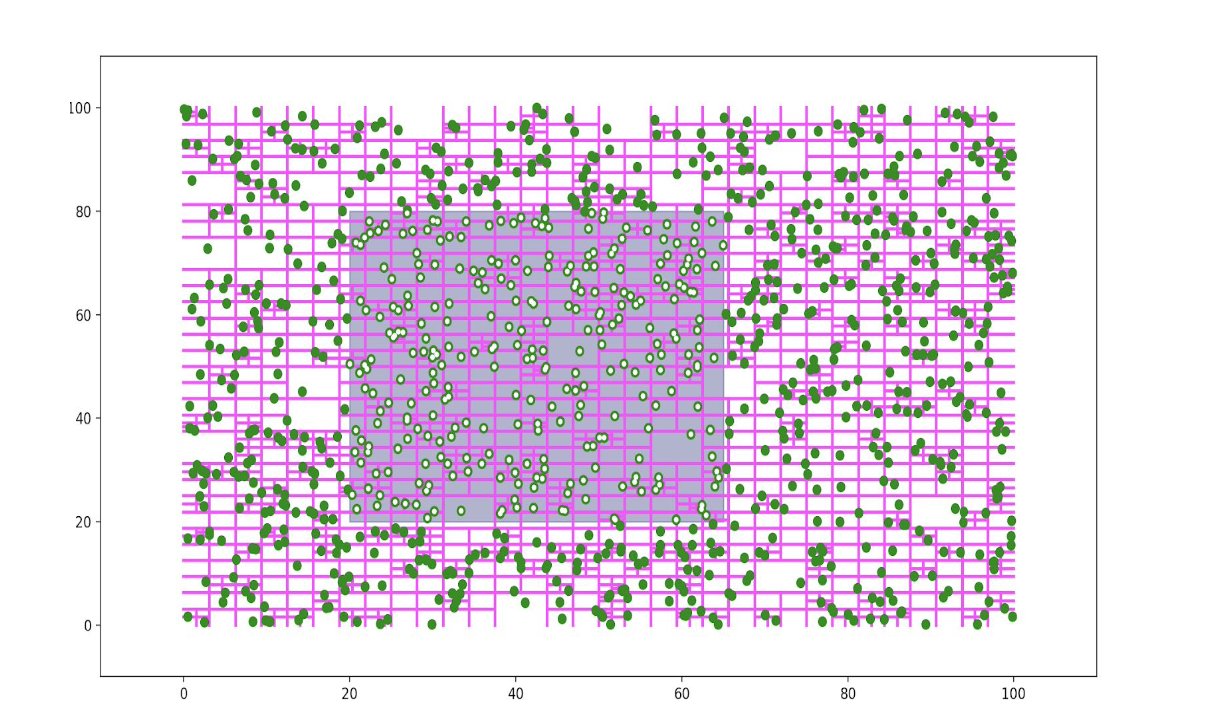
\includegraphics[width=\textwidth]{qrandom.png}
        \caption{Zbiór o rozkładzie jednostajnym QuadTree}
      \end{figure}

      \noindent
      \quad Jak widać na zamieszczonych ilustracjach, program działa prawidłowo zarówno przy użyciu QuadTree, jak i KDTree. 

      \noindent
      \quad Poniższa tabela ilustruje czasy działania programów dla podanego zbioru, przy danej ilości punktów:

      \begin{table}[h!]
      \centering
      \begin{center}
      \begin{tabular}{|c|c|c|c|c|}
          \hline
          \begin{tabular}{c} Liczba \\ punktów \end{tabular} & \begin{tabular}{c} Czas \\ tworzenia \\ KDTree [s] \end{tabular} & \begin{tabular}{c} Czas \\ przeszukiwania \\ KDTree [s] \end{tabular} & \begin{tabular}{c} Czas \\ tworzenia \\ QuadTree [s] \end{tabular} & \begin{tabular}{c} Czas \\ przeszukiwania \\ QuadTree [s] \end{tabular} \\
          \hline
          500 & 0.73491 & 0.00526 & 1.01075 & 0.00622 \\
          \hline
          1000 & 2.63573 & 0.00632 & 2.6174 & 0.00796 \\
          \hline
          1500 & 5.64069 & 0.00695 & 5.68459 & 0.00916 \\
          \hline
          2000 & 9.7806 & 0.00896 & 9.91145 & 0.01011 \\
          \hline
          2500 & 15.21827 & 0.01001 & 15.23907 & 0.01155 \\
          \hline
          3000 & 21.47649 & 0.01041 & 21.5799 & 0.01263 \\
          \hline
          3500 & 31.72233 & 0.01204 & 31.63304 & 0.01426 \\
          \hline
          4000 & 41.39933 & 0.0122 & 41.77491 & 0.01433 \\
          \hline
      \end{tabular}
      \end{center}
      \caption{Wyniki pomiarów czasu dla zbioru o rozkładzie jednostajnym}
      \end{table}

      \begin{figure}[h!]
      \centering
        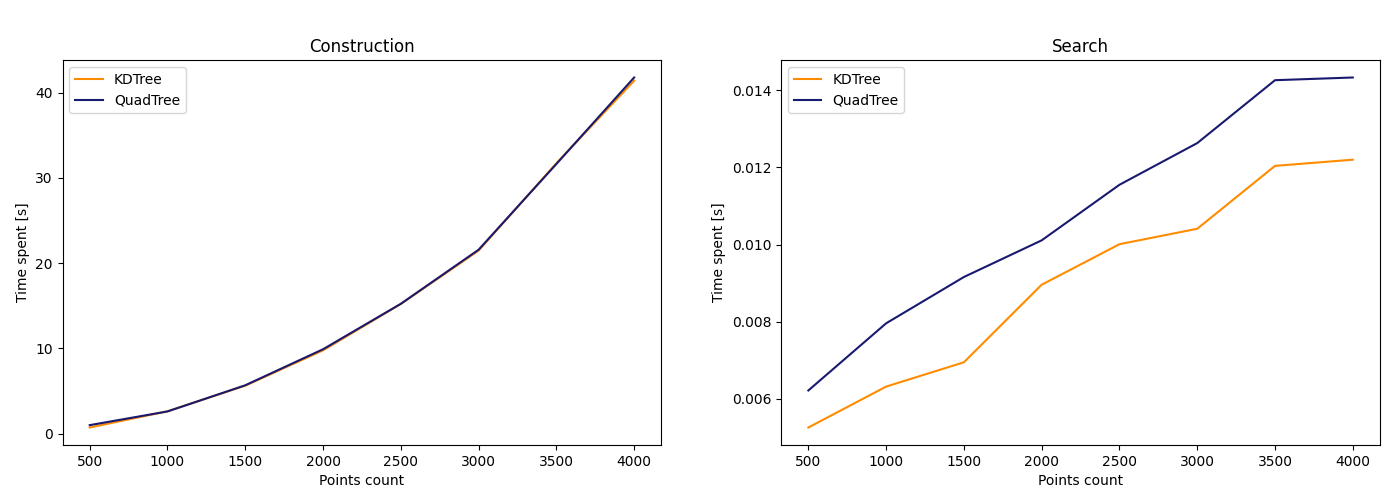
\includegraphics[width=\textwidth]{random.png}
        \caption{Wyniki pomiarów czasu dla zbioru o rozkładzie jednostajnym}
      \end{figure}

      \noindent
      \quad Na podstawie powyższej tabeli i wykresów możemy stwierdzić, że dla zbioru 1 tworzenie QuadTree i KDTree zajmuje jednakową ilość czasu. Natomiast przeszukiwanie QuadTree dla tego zbioru zajmuje średnio 20\% więcej czasu niż przeszukiwanie KDTree. 

    \subsection{Zbiór o rozkładzie normalnym}
      \quad Jest to zbiór punktów rozlokowany na płaszczyźnie zgodnie z rozkładem normalnym. Natomiast obszar, w którym mamy odnaleźć punkty to prostokąt zawierający część punktów należących do tego zbioru. Zbiór ten został wybrany ze względu na to, że jest on rozkładem bardzo powszechnym, więc uznaliśmy, że należy sprawdzić działanie naszych algorytmów dla tego zbioru. 

      \noindent
      \quad Poniższe ilustracje demonstrują wyniki działania programów dla 1000 punktów:

      \newpage
      \begin{figure}[h!]
      \centering
        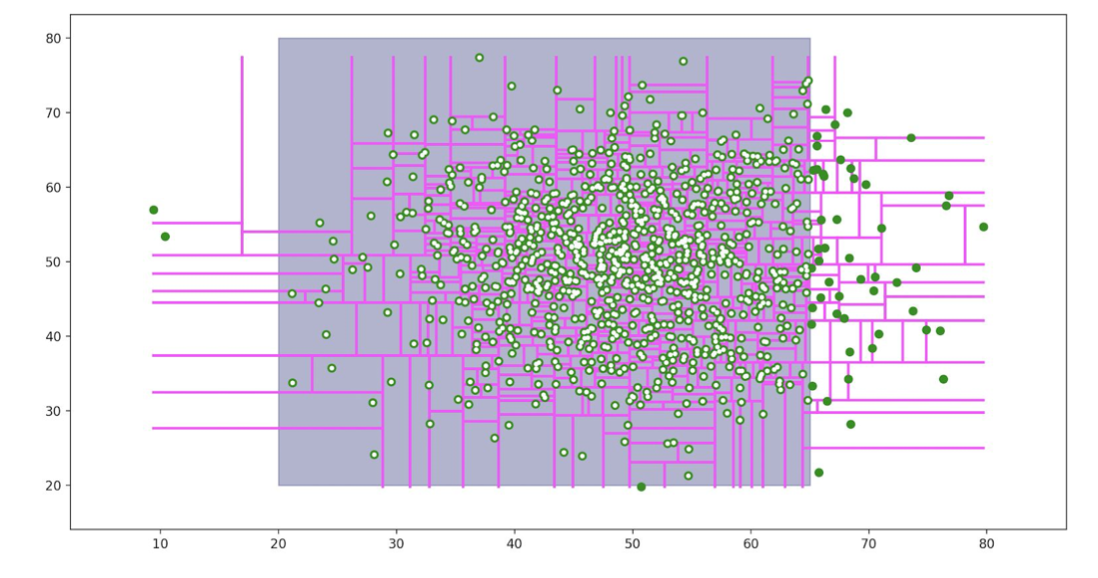
\includegraphics[width=0.97\textwidth]{knormal.png}
        \caption{Zbiór o rozkładzie normalnym KDTree}
      \end{figure}

      \begin{figure}[h!]
      \centering
        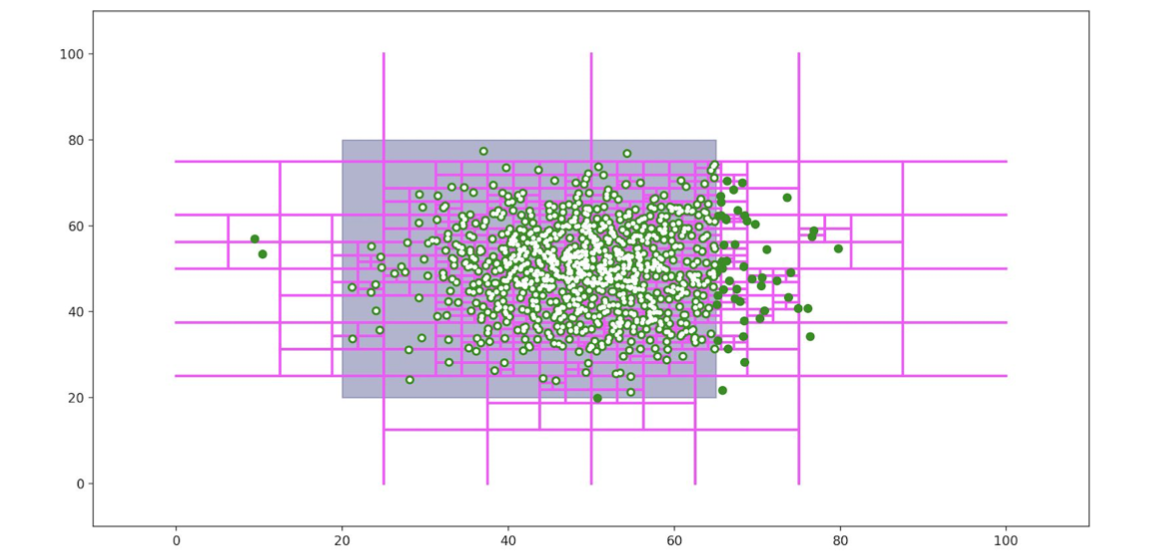
\includegraphics[width=\textwidth]{qnormal.png}
        \caption{Zbiór o rozkładzie normalnym QuadTree}
      \end{figure}

      \noindent
      \quad Jak widać na zamieszczonych ilustracjach, program działa prawidłowo zarówno przy użyciu QuadTree, jak i KDTree.

      \noindent
      \quad Poniższa tabela ilustruje czasy działania programów dla podanego zbioru, przy danej ilości punktów:

      \newpage
      \begin{table}[h!]
      \centering
      \begin{center}
      \begin{tabular}{|c|c|c|c|c|}
          \hline
          \begin{tabular}{c} Liczba \\ punktów \end{tabular} & \begin{tabular}{c} Czas \\ tworzenia \\ KDTree [s] \end{tabular} & \begin{tabular}{c} Czas \\ przeszukiwania \\ KDTree [s] \end{tabular} & \begin{tabular}{c} Czas \\ tworzenia \\ QuadTree [s] \end{tabular} & \begin{tabular}{c} Czas \\ przeszukiwania \\ QuadTree [s] \end{tabular} \\
          \hline
          500 & 0.65803 & 0.00393 & 0.71088 & 0.00349 \\
          \hline
          1000 & 2.59145 & 0.00529 & 2.66477 & 0.00494 \\
          \hline
          1500 & 5.64883 & 0.00684 & 5.69806 & 0.00601 \\
          \hline
          2000 & 9.8328 & 0.00939 & 9.95165 & 0.00627 \\
          \hline
          2500 & 15.19954 & 0.01015 & 15.3401 & 0.0078 \\
          \hline
          3000 & 22.13449 & 0.01187 & 23.23205 & 0.00985 \\
          \hline
          3500 & 30.74997 & 0.01341 & 31.08935 & 0.01013 \\
          \hline
          4000 & 41.94612 & 0.01568 & 41.49548 & 0.01302 \\
          \hline
      \end{tabular}
      \end{center}
      \caption{Wyniki pomiarów czasu dla zbioru o rozkładzie normalnym}
      \end{table}

      \begin{figure}[h!]
      \centering
        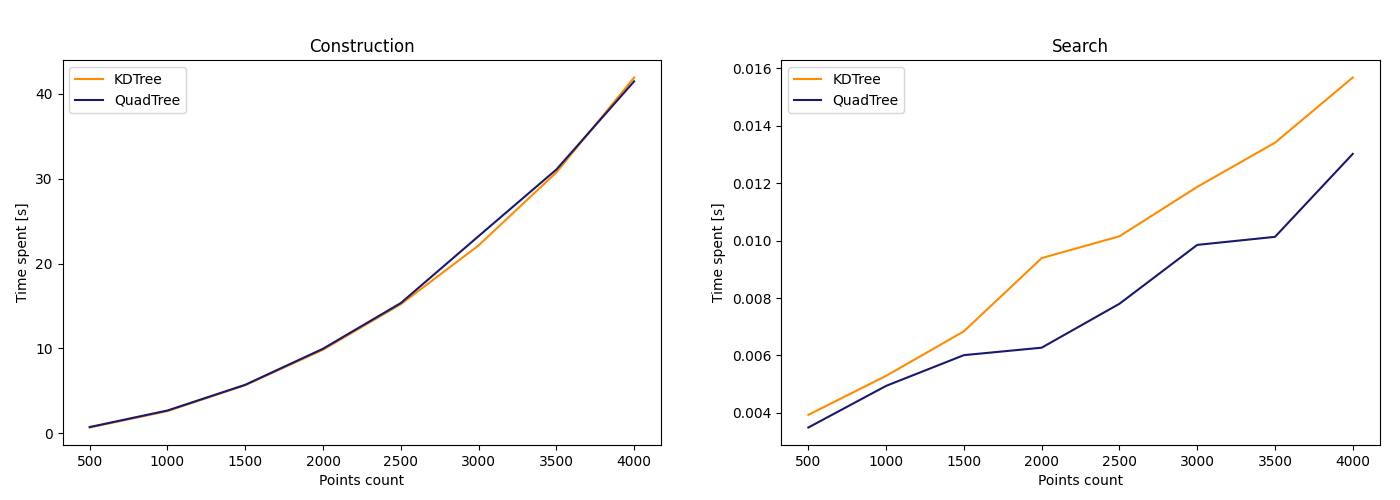
\includegraphics[width=\textwidth]{normal.png}
        \caption{Wyniki pomiarów czasu dla zbioru o rozkładzie normalnym}
      \end{figure}

      \noindent
      \quad Na podstawie powyższej tabeli i wykresów możemy stwierdzić, że dla zbioru 2 tworzenie QuadTree i KDTree zajmuje jednakową ilość czasu. Gdy liczba punktów w zbiorze nie przekracza 1500, przeszukiwanie KDTree dla tego zbioru  zajmuje średnio 10\% więcej czasu niż przeszukiwanie quadtree, w przeciwnym wypadku zajmuje ono ok. 25\% więcej czasu.

    \subsection{Siatka}
      \quad Jest to zbiór punktów należących do zadanego prostokąta, które odległe są od swoich sąsiadów o taką samą odległość. Punkty należące do zadanego zbioru są więc jednostajnie rozłożone na płaszczyźnie. Do tego prostokąt ten jest kwadratem o szerokości będącej potęgą dwójki (dlatego odległość pomiędzy sąsiadami w danej płaszczyźnie też jest potęgą dwójki). Natomiast obszar, w którym mamy odnaleźć punkty to prostokąt, częściowo przecinający nasz zbiór punktów. Warto zauważyć także, że poziomo jak i pionowo punkty te będą rozłożone na prostych zawierających identyczną ilość punktów, co mogłoby okazać się dla programu problematyczne. Należy też zwrócić uwagę, że w wypadku struktury QuadTree praktycznie każdy punkt będzie leżał na ramię prostokąta (ze względu na tak zadany zbiór punktów), co przy błędnej implementacji mogłoby spowodować przydzielenie danego punktu do więcej niż jednej części podziału, obecnie dzielonego prostokąta. Z powyższych powodów postanowiliśmy przetestować działanie naszych struktur także dla tego konkretnego zbioru punktów.

      \noindent
      \quad Poniższe ilustracje demonstrują wyniki działania programów dla punktów odległych od sąsiadów o 2 jednostki:

      \begin{figure}[h!]
      \centering
        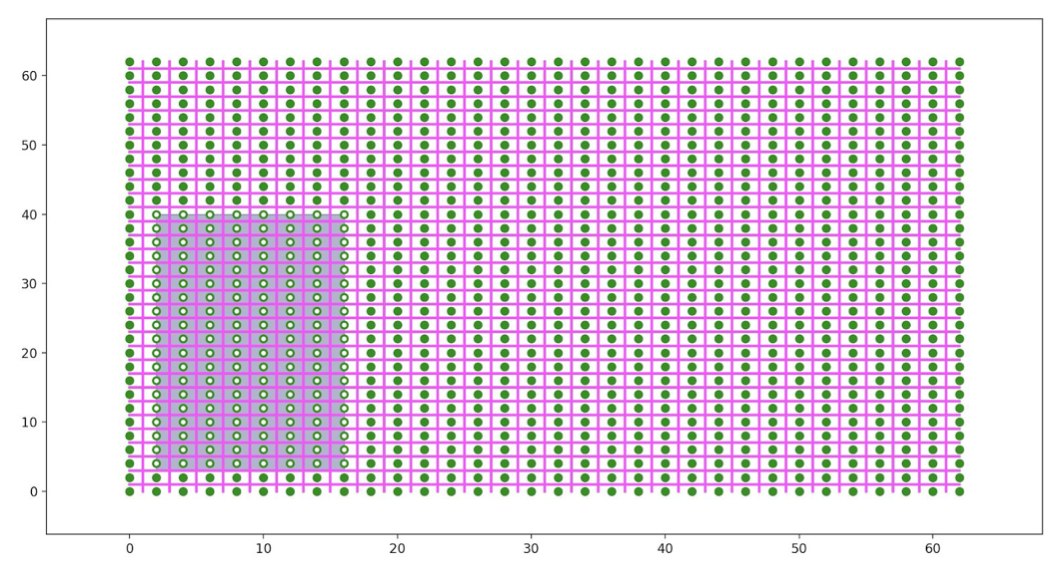
\includegraphics[width=\textwidth]{kgrid.png}
        \caption{Siatka KDTree}
      \end{figure}

      \begin{figure}[h!]
      \centering
        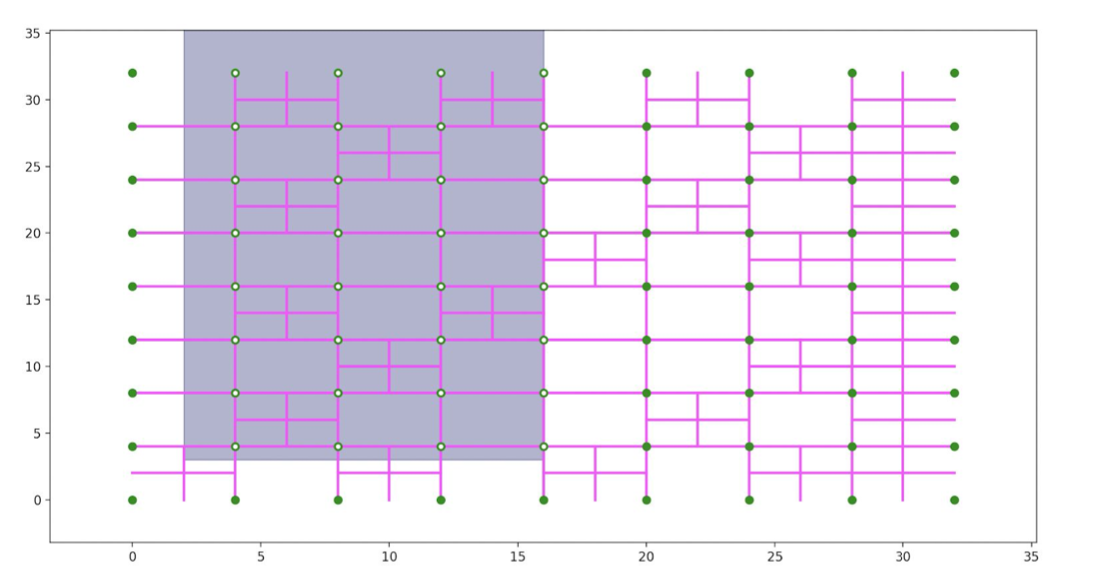
\includegraphics[width=\textwidth]{qgrid.png}
        \caption{Siatka QuadTree}
      \end{figure}

      \noindent
      \quad Jak widać na zamieszczonych ilustracjach, program działa prawidłowo zarówno przy użyciu QuadTree, jak i KDTree.

      \noindent
      \quad Poniższa tabela ilustruje czasy działania programów dla podanego zbioru, przy danej ilości punktów:

      \begin{table}[h!]
      \centering
      \begin{center}
      \begin{tabular}{|c|c|c|c|c|}
          \hline
          \begin{tabular}{c} Liczba \\ punktów \end{tabular} & \begin{tabular}{c} Czas \\ tworzenia \\ KDTree [s] \end{tabular} & \begin{tabular}{c} Czas \\ przeszukiwania \\ KDTree [s] \end{tabular} & \begin{tabular}{c} Czas \\ tworzenia \\ QuadTree [s] \end{tabular} & \begin{tabular}{c} Czas \\ przeszukiwania \\ QuadTree [s] \end{tabular} \\
          \hline
          81 & 0.0259 & 0.00146 & 0.02375 & 0.00145 \\
          \hline
          289 & 0.2503 & 0.00287 & 0.27596 & 0.00307 \\
          \hline
          1089 & 3.39618 & 0.00577 & 3.18027 & 0.00684 \\
          \hline
          4225 & 44.64996 & 0.01143 & 44.58075 & 0.01227 \\
          \hline
      \end{tabular}
      \end{center}
      \caption{Wyniki pomiarów czasu dla siatki}
      \end{table}

      \begin{figure}[h!]
      \centering
        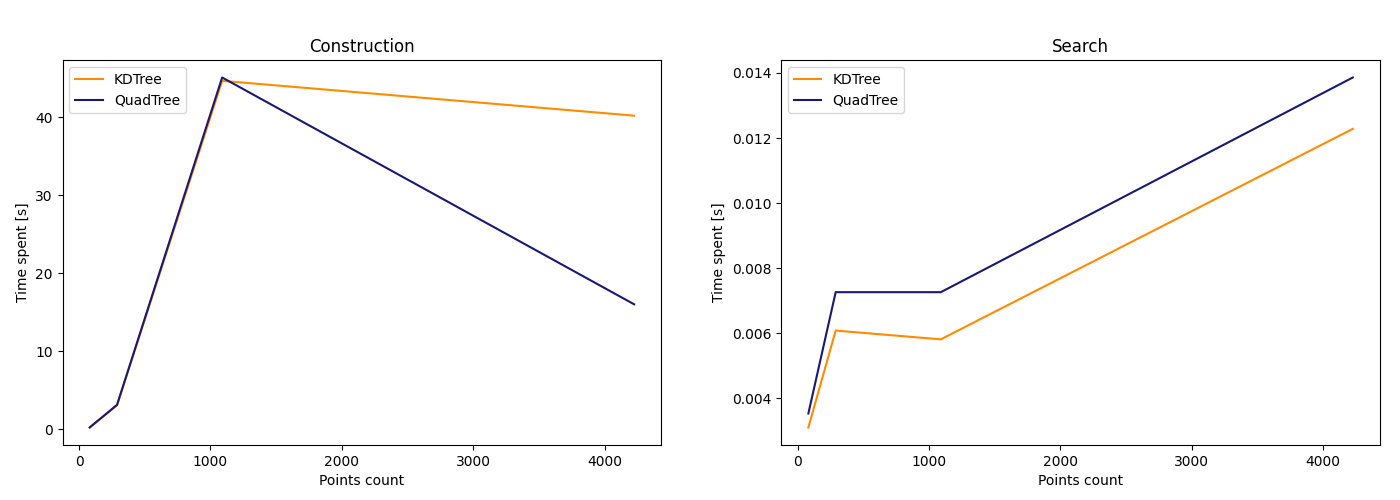
\includegraphics[width=\textwidth]{grid.png}
        \caption{Wyniki pomiarów czasu dla siatki}
      \end{figure}

      \noindent
      \quad Na podstawie powyższej tabeli i wykresów możemy stwierdzić, że dla zbioru 3 tworzenie QuadTree zajmuje średnio tyle samo czasu co tworzenie KDTree. Natomiast przeszukiwanie QuadTree dla tego zbioru zajmuje średnio 15\% więcej czasu niż przeszukiwanie KDTree. 

    \subsection{Klastry}
      \quad Jest to zbiór punktów złożony z czterech gęsto skoncentrowanych skupisk punktów. Zbiór ten sprawdza działanie programu, gdy punkty zamiast być jednostajnie rozłożone po całej płaszczyźnie, są skupione tylko w poszczególnych częściach prostokątnej płaszczyzny. Może to uwydatnić różnice w czasie działania, badanych przez nas struktur. Dla tego zbioru przetestujemy poszukiwanie punktów dla dwóch różnie zadanych prostokątów. Jednego, przecinającego skupiska punktów, drugiego, który zawiera w sobie wszystkie lub żadne punkty z danego skupiska. Zabieg ten ma na celu weryfikację czy program optymalnie wyszukuje punkty należące do danego prostokąta.

      \noindent
      \quad Poniższe ilustracje demonstrują wyniki działania programów dla 1000 punktów:

      \newpage
      \begin{figure}[h!]
      \centering
        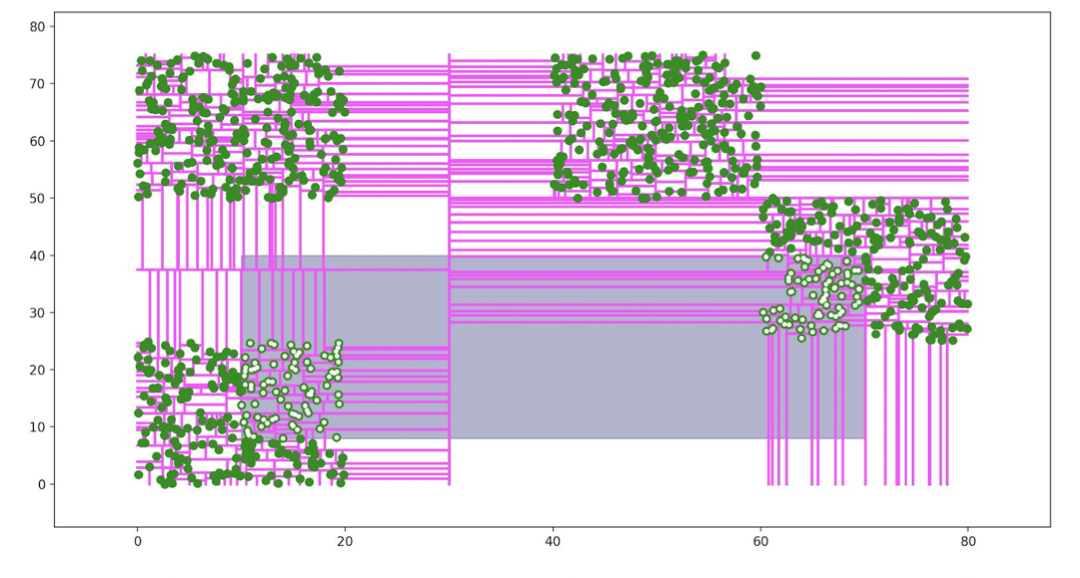
\includegraphics[width=\textwidth]{kclusters1.png}
        \caption{Klastry n1 KDTree}
      \end{figure}

      \begin{figure}[h!]
      \centering
        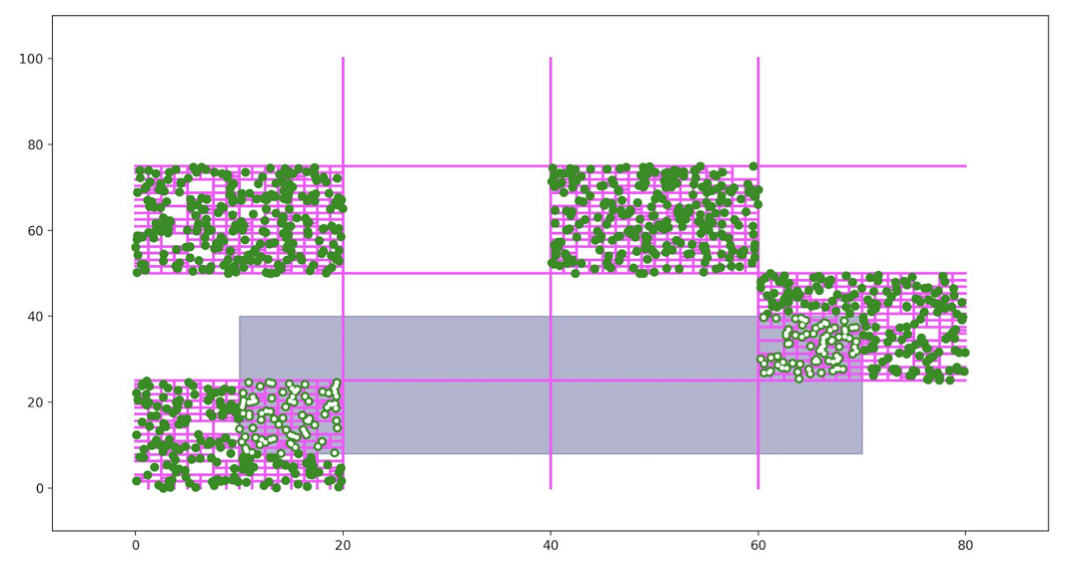
\includegraphics[width=\textwidth]{qclusters1.png}
        \caption{Klastry n1 QuadTree}
      \end{figure}

      \noindent
      \quad Jak widać na zamieszczonych powyżej i poniżej ilustracjach, program działa prawidłowo zarówno przy użyciu QuadTree, jak i KDTree.

      \newpage
      \begin{figure}[h!]
      \centering
        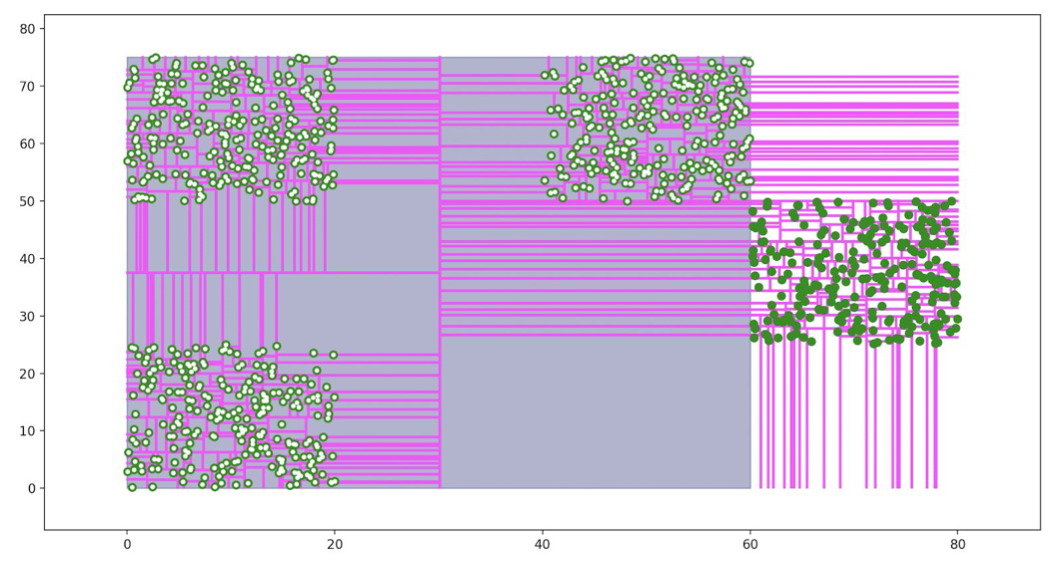
\includegraphics[width=\textwidth]{kclusters2.png}
        \caption{Klastry n2 KDTree}
      \end{figure}

      \begin{figure}[h!]
      \centering
        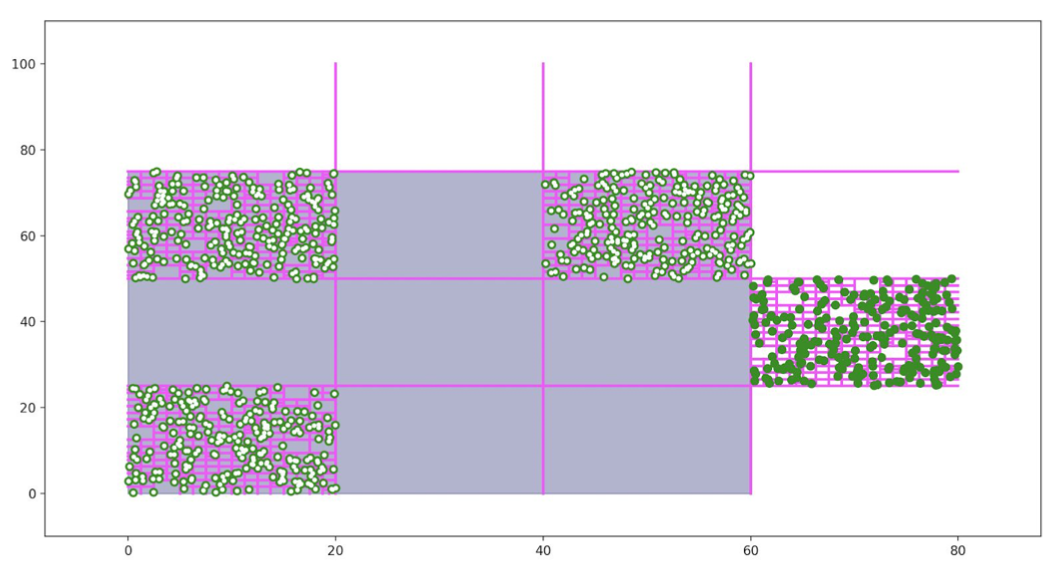
\includegraphics[width=\textwidth]{qclusters2.png}
        \caption{Klastry n2 QuadTree}
      \end{figure}

      \noindent
      \quad Poniższa tabela ilustruje czasy działania programów dla podanego zbioru, przy danej ilości punktów (odpowiednio niżej są przedstawione wykresy):

      \newpage
      \begin{table}[h!]
      \centering
      \begin{center}
      \begin{tabular}{|c|c|c|c|c|}
          \hline
          \begin{tabular}{c} Liczba \\ punktów \end{tabular} & \begin{tabular}{c} Czas \\ tworzenia \\ KDTree [s] \end{tabular} & \begin{tabular}{c} Czas \\ przeszukiwania \\ KDTree [s] \end{tabular} & \begin{tabular}{c} Czas \\ tworzenia \\ QuadTree [s] \end{tabular} & \begin{tabular}{c} Czas \\ przeszukiwania \\ QuadTree [s] \end{tabular} \\
          \hline
          500 & 0.68132 & 0.00313 & 0.6991 & 0.0031 \\
          \hline
          1000 & 2.56068 & 0.0046 & 2.62753 & 0.00402 \\
          \hline
          1500 & 5.61545 & 0.00552 & 5.70088 & 0.005 \\
          \hline
          2000 & 9.84998 & 0.00579 & 9.98057 & 0.00498 \\
          \hline
          2500 & 15.16315 & 0.00737 & 15.28278 & 0.00597 \\
          \hline
          3000 & 22.87313 & 0.0077 & 22.01085 & 0.00634 \\
          \hline
          3500 & 31.16272 & 0.00837 & 31.99417 & 0.00731 \\
          \hline
          4000 & 41.27115 & 0.00989 & 42.60962 & 0.00842 \\
          \hline
      \end{tabular}
      \end{center}
      \caption{Wyniki pomiarów czasu dla klaster n1}
      \end{table}

      \begin{figure}[h!]
      \centering
        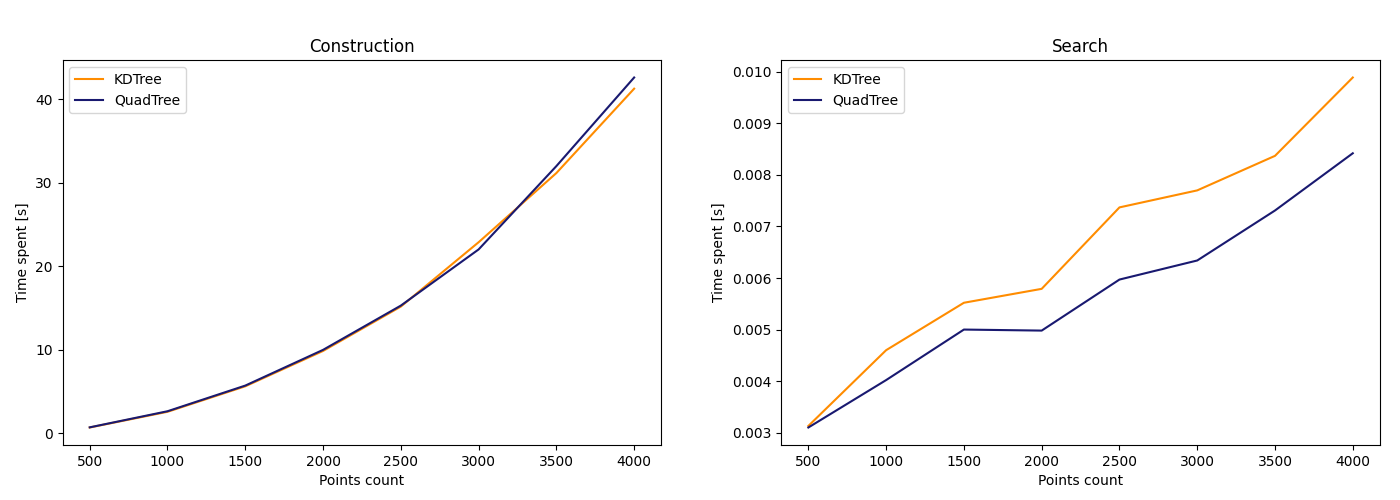
\includegraphics[width=\textwidth]{clusters1.png}
        \caption{Wyniki pomiarów czasu dla klaster n1}
      \end{figure}

      \begin{table}[h!]
      \centering
      \begin{center}
      \begin{tabular}{|c|c|c|c|c|}
          \hline
          \begin{tabular}{c} Liczba \\ punktów \end{tabular} & \begin{tabular}{c} Czas \\ tworzenia \\ KDTree [s] \end{tabular} & \begin{tabular}{c} Czas \\ przeszukiwania \\ KDTree [s] \end{tabular} & \begin{tabular}{c} Czas \\ tworzenia \\ QuadTree [s] \end{tabular} & \begin{tabular}{c} Czas \\ przeszukiwania \\ QuadTree [s] \end{tabular} \\
          \hline
          500 & 0.67177 & 0.00257 & 0.68885 & 0.00141 \\
          \hline
          1000 & 2.59746 & 0.00375 & 2.74539 & 0.00245 \\
          \hline
          1500 & 5.61685 & 0.00479 & 5.7088 & 0.00303 \\
          \hline
          2000 & 9.82799 & 0.00582 & 9.94246 & 0.00357 \\
          \hline
          2500 & 15.26792 & 0.0065 & 15.23768 & 0.00334 \\
          \hline
          3000 & 22.00586 & 0.0072 & 21.81148 & 0.00402 \\
          \hline
          3500 & 32.48849 & 0.00918 & 32.4198 & 0.00536 \\
          \hline
          4000 & 42.63721 & 0.00946 & 42.17839 & 0.00821 \\
          \hline
      \end{tabular}
      \end{center}
      \caption{Wyniki pomiarów czasu dla klaster n2}
      \end{table}

      \begin{figure}[h!]
      \centering
        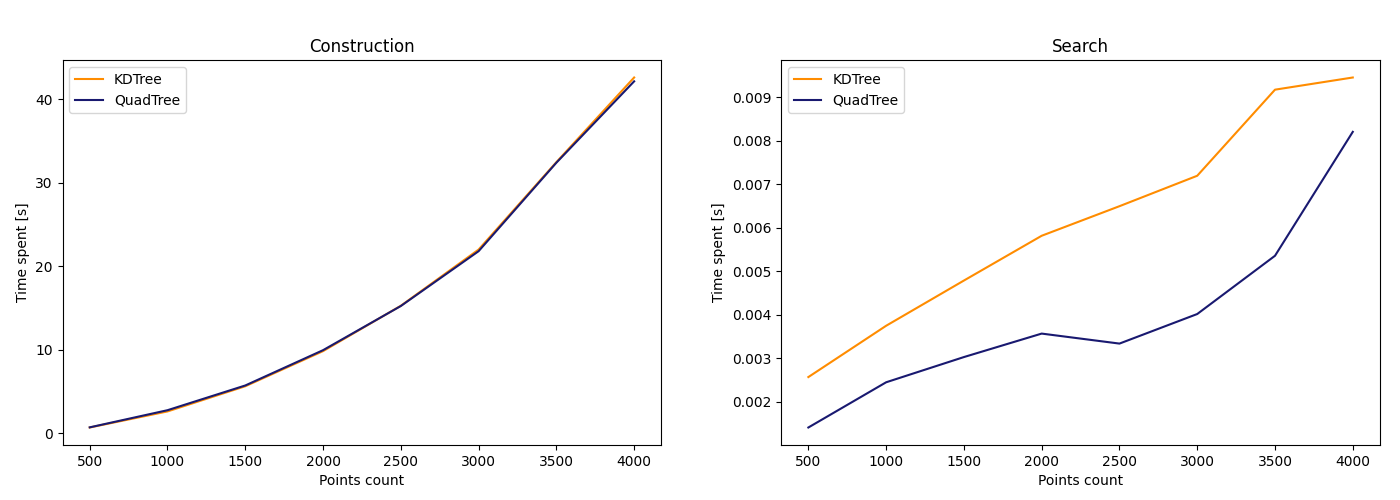
\includegraphics[width=\textwidth]{clusters2.png}
        \caption{Wyniki pomiarów czasu dla klaster n2}
      \end{figure}

      \noindent
      \quad Na podstawie powyższych tabel i wykresów (ostatni jest na nast. stronie) możemy stwierdzić, że dla zbioru 4 tworzenie QuadTree zajmuje średnio tyle samo czasu co KDTree. Gdy liczba punktów w zbiorze nie przekracza 2000, przeszukiwanie KDTree dla obszaru przeszukiwanego nr 1  zajmuje średnio 10\% więcej czasu niż przeszukiwanie QuadTree, w przeciwnym wypadku zajmuje ono ok. 20\% więcej czasu. Natomiast dla obszaru przeszukiwanego nr 2, przeszukiwanie KDTree zajmuje 60-80\%  więcej czasu niż przeszukiwanie QuadTree. Możemy zauważyć, że QuadTree działa w drugim przypadku zdecydowanie szybciej od KDTree, dzieje się to na skutek tego, że w tym wypadku QuadTree odcina węzły znacznie szybciej (“płyciej”) od KDTree, co bezpośrednio wpływa na szybkość przeszukiwania drzewa . 

    \subsection{Wartości odstające (outliers)}
      \quad Mamy dwa różne zbiory tutaj:

      \begin{itemize}
          \item \textbf{Zbiór 5.1} Jest to zbiór, którego 99\% punktów należy do konkretnego skupiska punktów (niewielkiego obszaru będącego częścią zadanego zbioru), a pozostałe punkty są losowo rozmieszczone na zadanym zbiorze. Natomiast obszar, w którym mamy odnaleźć punkty to prostokąt, częściowo przecinający skupisko, w którym znajduje się 99\% punktów naszego zbioru. 

          \item \textbf{Zbiór 5.2} Jest to zbiór gdzie 3 jego punkty leżą na wierzchołkach zadanego prostokąta o bardzo dużych wymiarach w porównaniu do wymiarów prostokąta z resztą, a właśnie reszta punktów leży skupiona w niewielkim obszarze obok czwartego wierzchołka tego prostokąta. Natomiast obszar, w którym mamy odnaleźć punkty to prostokąt częściowo przecinający skupisko punktów i nie przecinający punktów leżących na pozostałych wierzchołkach.
      \end{itemize}

      \noindent
      \quad Zbiory te zostały wybrany ze względu na to, że mogą być one problematyczne dla QuadTree, warto więc przeanalizować ten charakterystyczny rozkład punktów, szczególnie zwracając uwagę na różnice w czasie działania QuadTree i KDTree. 

      \noindent
      \quad Poniższe ilustracje demonstrują wyniki działania programów dla 1000 punktów:

      \newpage
      \begin{figure}[h!]
      \centering
        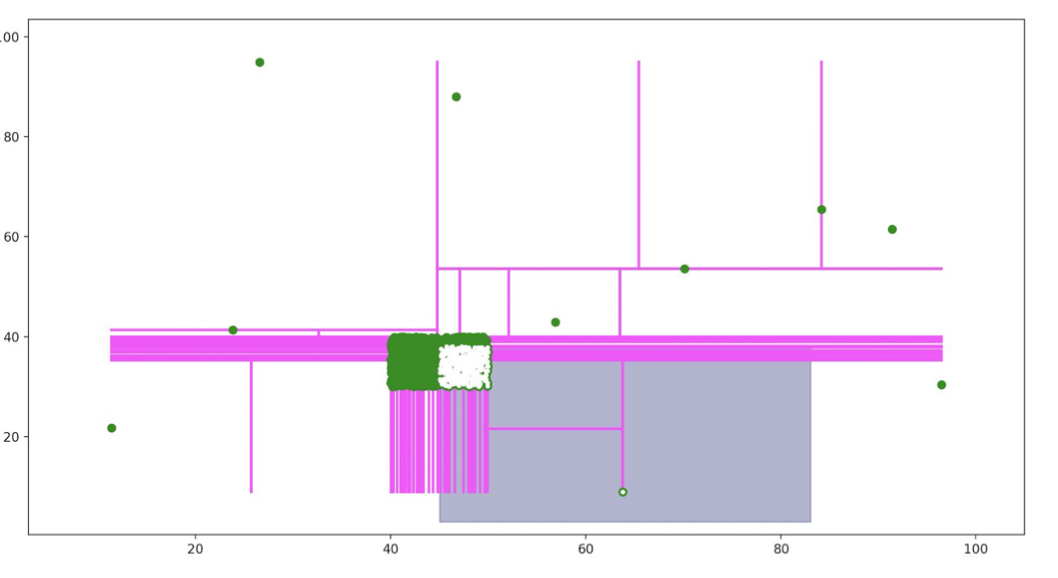
\includegraphics[width=\textwidth]{koutliers1.png}
        \caption{Wartości odstające n1 KDTree}
      \end{figure}

      \begin{figure}[h!]
      \centering
        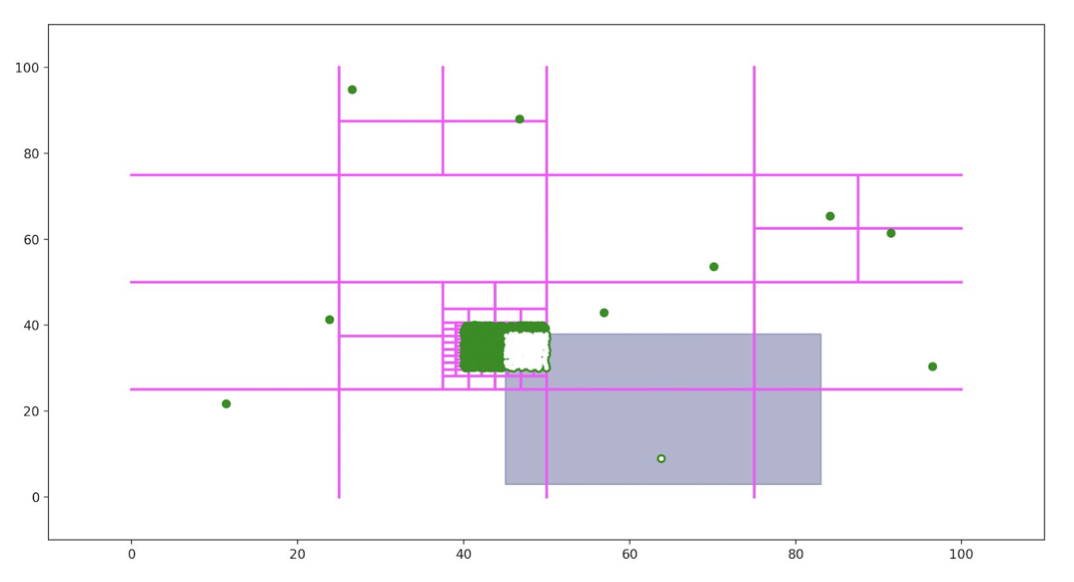
\includegraphics[width=\textwidth]{qoutliers1.png}
        \caption{Wartości odstające n1 QuadTree}
      \end{figure}

      \noindent
      \quad Jak widać na zamieszczonych powyżej i poniżej ilustracjach, program działa prawidłowo zarówno przy użyciu QuadTree, jak i KDTree.

      \newpage
      \begin{figure}[h!]
      \centering
        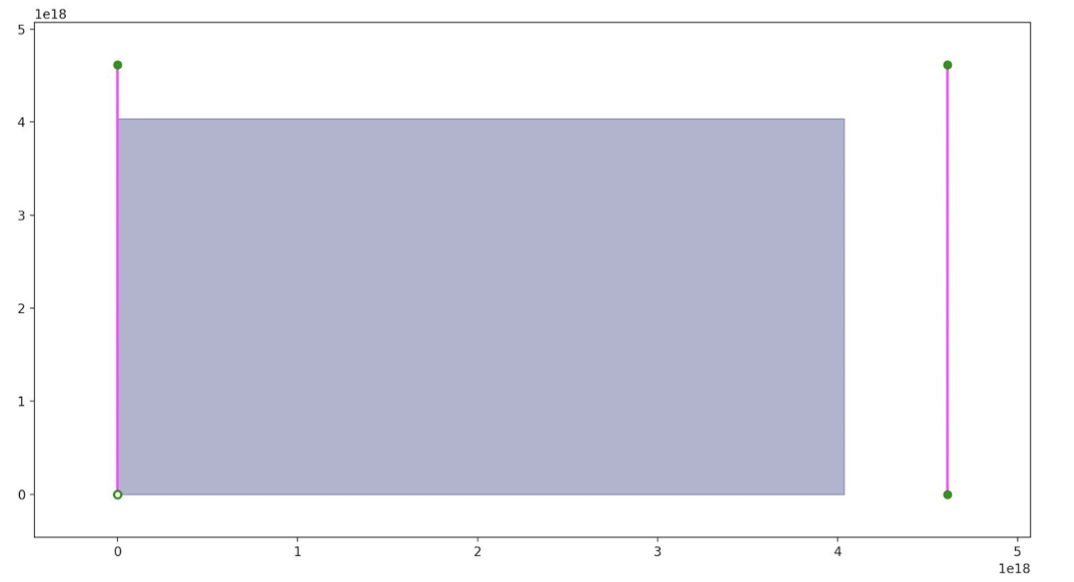
\includegraphics[width=\textwidth]{koutliers2.png}
        \caption{Wartości odstające n2 KDTree}
      \end{figure}

      \begin{figure}[h!]
      \centering
        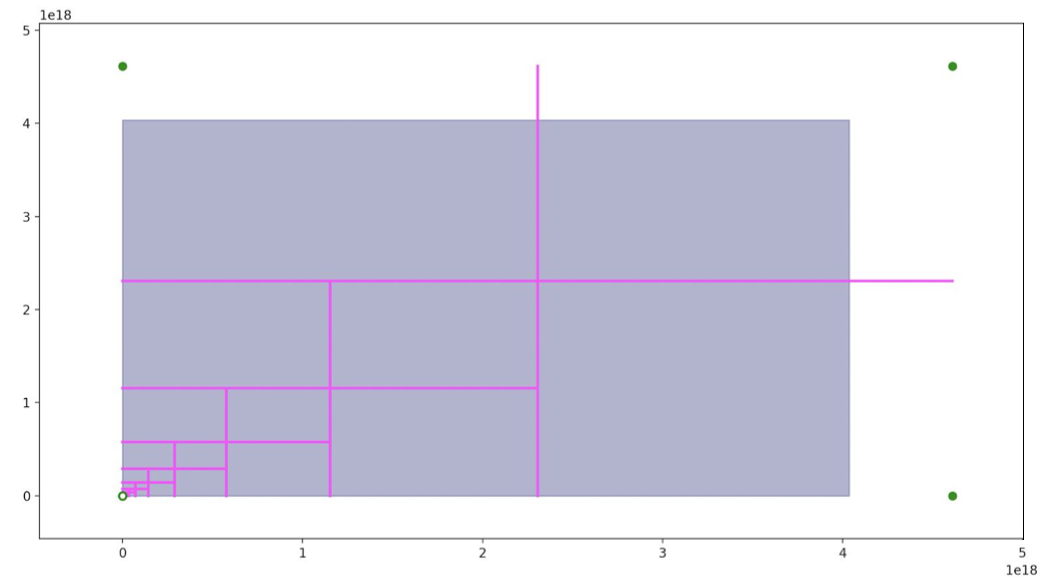
\includegraphics[width=\textwidth]{qoutliers2.png}
        \caption{Wartości odstające n2 QuadTree}
      \end{figure}

      \noindent
      \quad Poniższa tabela i wykresy ilustruje czasy działania programów dla podanego zbioru, przy danej ilości punktów:

      \newpage
      \begin{table}[h!]
      \centering
      \begin{center}
      \begin{tabular}{|c|c|c|c|c|}
          \hline
          \begin{tabular}{c} Liczba \\ punktów \end{tabular} & \begin{tabular}{c} Czas \\ tworzenia \\ KDTree [s] \end{tabular} & \begin{tabular}{c} Czas \\ przeszukiwania \\ KDTree [s] \end{tabular} & \begin{tabular}{c} Czas \\ tworzenia \\ QuadTree [s] \end{tabular} & \begin{tabular}{c} Czas \\ przeszukiwania \\ QuadTree [s] \end{tabular} \\
          \hline
          500 & 0.91441 & 0.00496 & 0.83041 & 0.00788 \\
          \hline
          1000 & 2.57154 & 0.00589 & 2.68101 & 0.00485 \\
          \hline
          1500 & 5.56844 & 0.00704 & 5.76521 & 0.0051 \\
          \hline
          2000 & 9.77039 & 0.0089 & 10.02134 & 0.00652 \\
          \hline
          2500 & 15.20645 & 0.00902 & 15.35985 & 0.00824 \\
          \hline
          3000 & 20.51018 & 0.00996 & 22.12177 & 0.00848 \\
          \hline
          3500 & 31.29155 & 0.00975 & 33.43466 & 0.0097 \\
          \hline
          4000 & 42.39134 & 0.01036 & 40.8002 & 0.01033 \\
          \hline
      \end{tabular}
      \end{center}
      \caption{Wyniki pomiarów czasu dla wartości odstających n1}
      \end{table}

      \begin{figure}[h!]
      \centering
        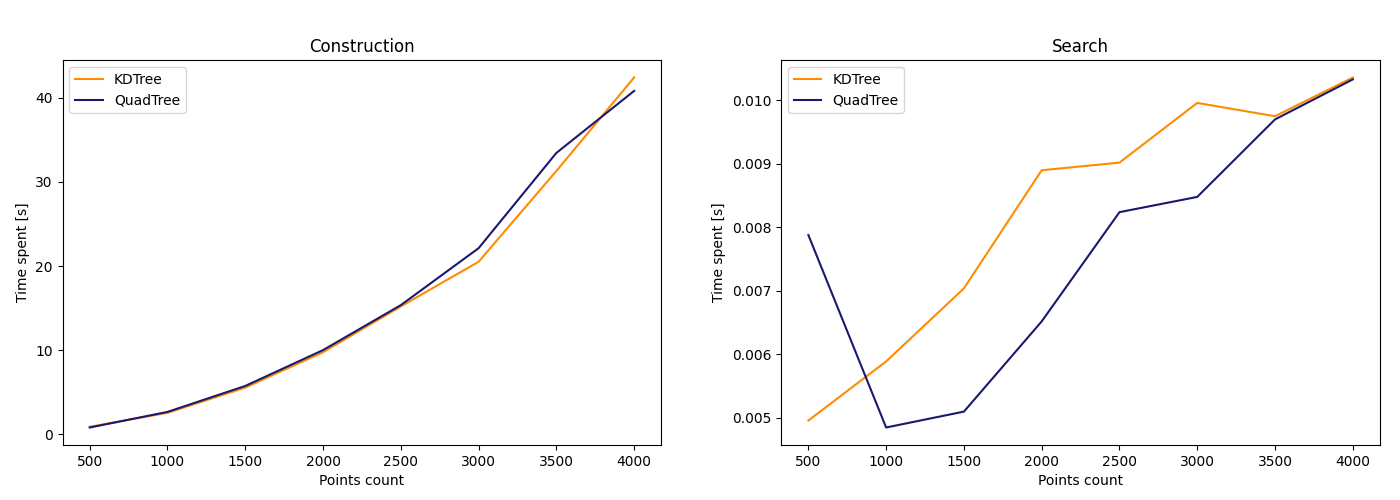
\includegraphics[width=\textwidth]{outliers1.png}
        \caption{Wyniki pomiarów czasu dla wartości odstających n1}
      \end{figure}

      \noindent
      \quad Zbiory o liczbie 500 i 1000 punktów nie są brane pod uwagę w poniższej analizie, ponieważ ze względu na charakterystykę tego zbioru jest to za mała liczba punktów, aby uzyskać  rzetelne wyniki odpowiednie do wyciągania z nich wniosków. Na podstawie powyższej tabeli i wykresów możemy stwierdzić, że dla zbioru 5.1 tworzenie QuadTree zajmuje tyle samo czasu co KDTree . Natomiast różnica czasów przeszukiwania tych struktur zależy od ilości punktów. Im więcej punktów tym lepiej (pod względem szybkości) wypada KDTree. Dla 1500 punktów KDTree jest przeszukiwane 40\% dłużej od QuadTree, natomiast dla 4000 punktów czas przeszukiwania tych dwóch struktur jest niemal identyczny, możemy przewidywać, że dla większej ilości punktów KDTree będzie przeszukiwane szybciej niż QuadTree. 

      \newpage
      \begin{table}[h!]
      \centering
      \begin{center}
      \begin{tabular}{|c|c|c|c|c|}
          \hline
          \begin{tabular}{c} Liczba \\ punktów \end{tabular} & \begin{tabular}{c} Czas \\ tworzenia \\ KDTree [s] \end{tabular} & \begin{tabular}{c} Czas \\ przeszukiwania \\ KDTree [s] \end{tabular} & \begin{tabular}{c} Czas \\ tworzenia \\ QuadTree [s] \end{tabular} & \begin{tabular}{c} Czas \\ przeszukiwania \\ QuadTree [s] \end{tabular} \\
          \hline
          500 & 0.8176 & 0.00316 & 1.40296 & 0.00669 \\
          \hline
          1000 & 2.57741 & 0.00509 & 4.05358 & 0.00746 \\
          \hline
          1500 & 5.59511 & 0.00684 & 7.9869 & 0.00842 \\
          \hline
          2000 & 9.8141 & 0.00748 & 12.78849 & 0.0087 \\
          \hline
          2500 & 15.1543 & 0.00761 & 18.92475 & 0.0099 \\
          \hline
          3000 & 21.93263 & 0.00805 & 26.28272 & 0.00964 \\
          \hline
          3500 & 31.30687 & 0.01025 & 36.22217 & 0.01056 \\
          \hline
          4000 & 40.10829 & 0.01087 & 47.38874 & 0.01154 \\
          \hline
      \end{tabular}
      \end{center}
      \caption{Wyniki pomiarów czasu dla wartości odstających n2}
      \end{table}

      \begin{figure}[h!]
      \centering
        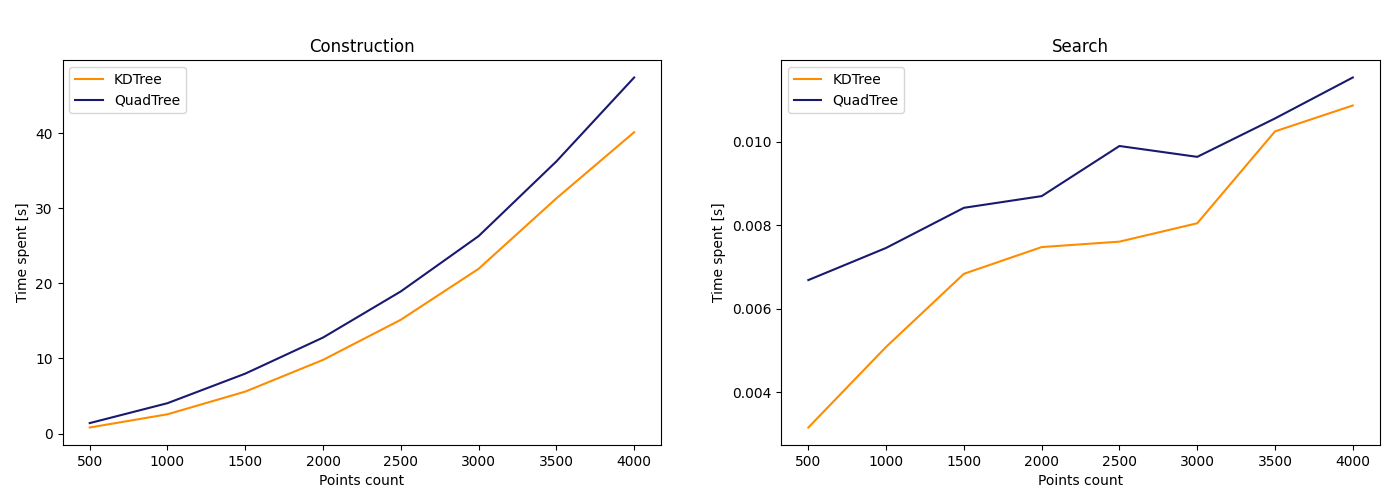
\includegraphics[width=\textwidth]{outliers2.png}
        \caption{Wyniki pomiarów czasu dla wartości odstających n2}
      \end{figure}

      \noindent
      \quad Na podstawie powyższej tabeli i wykresów możemy stwierdzić, że dla zbioru 5.2 tworzenie QuadTree zajmuje 20\% dłużej niż KDTree . Natomiast różnica czasów przeszukiwania tych struktur zależy od ilości punktów. Im więcej punktów tym lepiej (pod względem szybkości) wypada QuadTree. Dla 500 punktów QuadTree jest przeszukiwane 2 razy dłużej od KDTree (dzieje się to dlatego, że punkty na kątach prostokąta są rzędu $2^{62}$, więc QuadTree musi zejść bardzo głęboko, żeby dostać się do reszty punktów zawartych w obszarze $[0, 100]^2$. Dla 4000 punktów czas przeszukiwania QuadTree jest już tylko niecałe 10\% dłuższy niż czas przeszukiwania KDTree. Możemy przewidywać, że dla większej ilości punktów QuadTree będzie przeszukiwane szybciej niż KDTree. Jest to dlatego, że KDTree tworzy duższe rozgałęzienie pionowe i poziomowe, które zaczepia praktycznie całą stronę prostokąta, który jest bardzo duży. Potwierdzeniem jest pionowa linia podziału na rysunku 30. QuadTree w tym czasie nie komplikuje swojej struktury zewnątrz prostokąta zawierającego obszar $[0, 100]^2$. Więc zmienia prędkość tak, jakby dla zbioru o rozkładzie jednostajnym.

    \subsection{Krzyż}
      \quad Jest to zbiór punktów należących do dwóch prostych będących osiami symetrii zadanego prostokąta. Przecinają się one w środku symetrii prostokąta. Natomiast obszar, w którym mamy odnaleźć punkty to prostokąt zawierający fragmenty obydwóch prostych (więc i środek symetrii). Wybrany został ten zbiór punktów ze względu na to, że punkty należące do niego znajdują się tylko na dwóch prostych i to tych dzielących prostokąt na dwie równe części, co może być problematyczne dla działania programów, w związku z tym istnieje duże prawdopodobieństwo wykrycia błędów jeżeli takie program posiada. Z tego powodu postanowiliśmy przeanalizować także ten szczególny zbiór punktów. 

      \noindent
      \quad Poniższe ilustracje demonstrują wyniki działania programów dla 1000 punktów:

      \begin{figure}[h!]
      \centering
        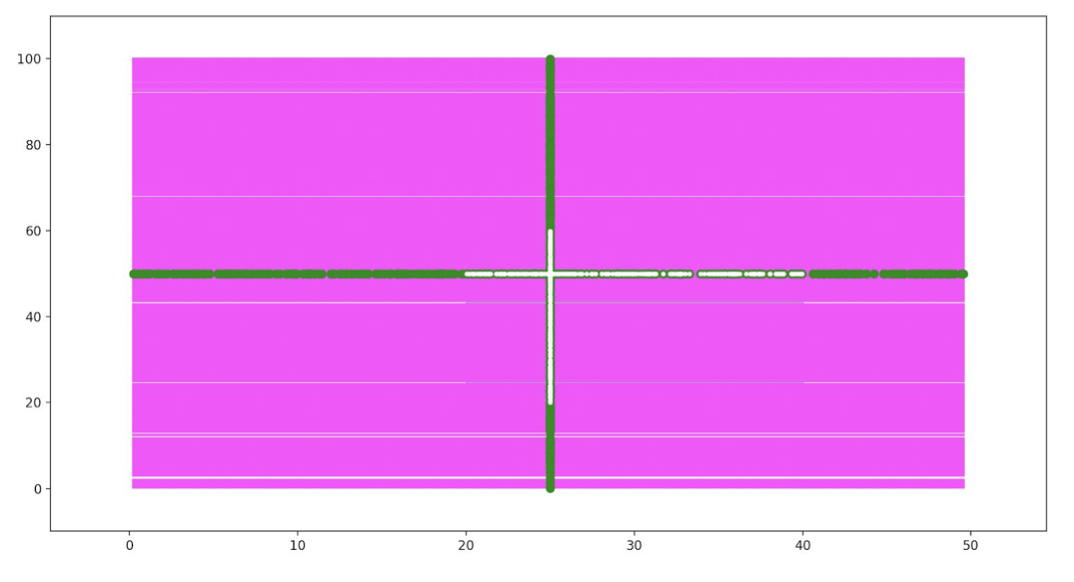
\includegraphics[width=0.9\textwidth]{kcross.png}
        \caption{Krzyż KDTree}
      \end{figure}

      \begin{figure}[h!]
      \centering
        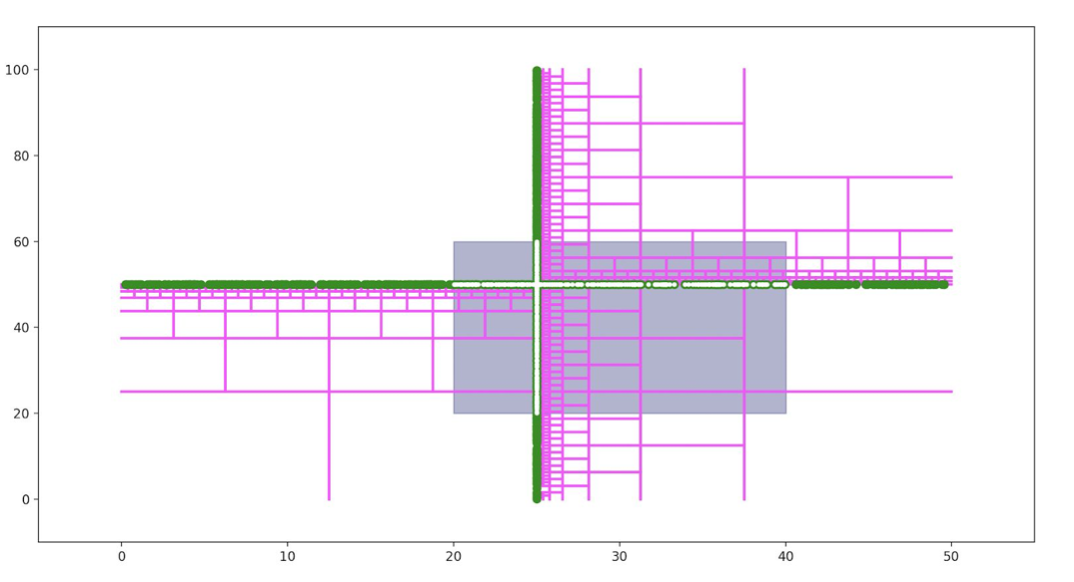
\includegraphics[width=0.9\textwidth]{qcross.png}
        \caption{Krzyż QuadTree}
      \end{figure}

      \noindent
      \quad Jak widać na zamieszczonych ilustracjach, program działa prawidłowo zarówno przy użyciu QuadTree, jak i KDTree.

      \noindent
      \quad Poniższa tabela i wykresy ilustrują czasy działania programów dla podanego zbioru, przy danej ilości punktów:

      \begin{table}[h!]
      \centering
      \begin{center}
      \begin{tabular}{|c|c|c|c|c|}
          \hline
          \begin{tabular}{c} Liczba \\ punktów \end{tabular} & \begin{tabular}{c} Czas \\ tworzenia \\ KDTree [s] \end{tabular} & \begin{tabular}{c} Czas \\ przeszukiwania \\ KDTree [s] \end{tabular} & \begin{tabular}{c} Czas \\ tworzenia \\ QuadTree [s] \end{tabular} & \begin{tabular}{c} Czas \\ przeszukiwania \\ QuadTree [s] \end{tabular} \\
          \hline
          500 & 0.67863 & 0.00398 & 0.74997 & 0.00249 \\
          \hline
          1000 & 2.59964 & 0.0121 & 2.7639 & 0.00314 \\
          \hline
          1500 & 5.57651 & 0.01075 & 5.92202 & 0.00293 \\
          \hline
          2000 & 9.86725 & 0.01531 & 10.25673 & 0.00332 \\
          \hline
          2500 & 15.20696 & 0.01822 & 15.69262 & 0.00329 \\
          \hline
          3000 & 21.8318 & 0.02045 & 22.28464 & 0.00352 \\
          \hline
          3500 & 32.82205 & 0.02588 & 33.4228 & 0.00407 \\
          \hline
          4000 & 42.91555 & 0.04264 & 43.52262 & 0.00544 \\
          \hline
      \end{tabular}
      \end{center}
      \caption{Wyniki pomiarów czasu dla krzyża}
      \end{table}

      \begin{figure}[h!]
      \centering
        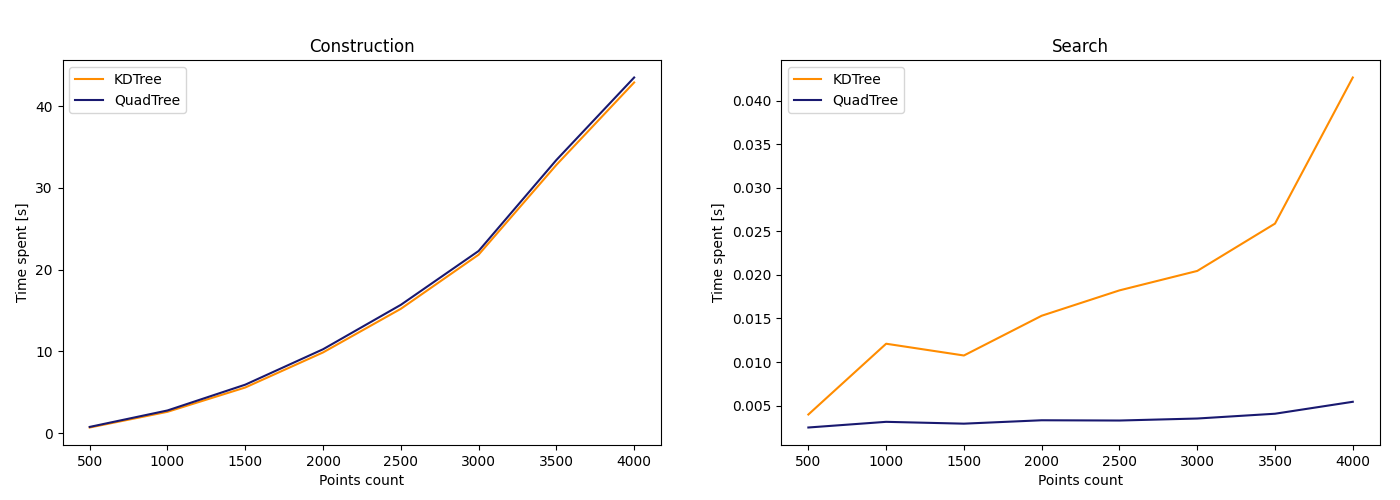
\includegraphics[width=\textwidth]{cross.png}
        \caption{Wyniki pomiarów czasu dla krzyża}
      \end{figure}

      \noindent
      \quad Na podstawie powyższej tabeli i wykresów możemy stwierdzić, że dla zbioru 6 tworzenie QuadTree zajmuje średnio tyle samo czasu co KDTree . Natomiast różnica czasów przeszukiwania tych struktur zależy od ilości punktów. Dla 500 punktów przeszukiwanie KDTree działa 60\% dłużej od przeszukiwania QuadTree, dla 1000 punktów działa 4 razy dłużej, a dla 4000 punktów działa 8 razy dłużej. Oznacza to, że im bardziej konsystentnie punkty tworzą proste, tym różnica czasów jest coraz większa. Możemy, więc stwierdzić, że dla tak zadanego zbioru przeszukiwanie QuadTree działa znacznie szybciej od przeszukiwania KDTree. 

      \noindent
      \quad Właśnie dlatego ten zbiór i został wybrany, że ilustruje jeden duży problem KDTree - linie równoległe do osi. Dla przypadku gdy mamy 100 punktów z prostej równoległej do OX, i 101 punktów z prostej równoległej do OY, i załóżmy, że rozstęp punktów z osi równoległej do OX (dalej 'x') jest większy, to podzielimy według $x$. O ile 101 punkt jest z prostej równoległej do OY (dalej 'y'), to wybierzemy ten punkt podziału, a jeżeli założymy, że wartości $x$ dla wszystkich punktów z prostej 'x' oprócz jednego są mniejsze od wartości $x$ dla 'y', to odcinamy tylko jeden punkt i zostawiamy 200, co już nie wygląda na bardzo wydajną strukturę. 

      \noindent
      \quad Jeszcze większy problem będzie, jeżeli wartości $x$ wszystkich punktów z prostej 'x' będą mniejsze od punktów z 'y'. Wtedy wszystkie punkty zakwalifikuje do lewego poddrzewa, i tak wejdziemy w nieskończoną rekurencję, bo zawsze będziemy próbowali rozbić ten sam zbiór punktów, który pozostaje niezmienny za każdym razem. Jest to rozwiązane w taki sposób, że jak ilość punktów nie zmienia się, to warunek '$<=$' staje się '$<$'. A o ile korzystamy z funkcji anonimowych, które zwracają nam \textbf{True}, jeżeli idziemy do lewego poddrzewa i \textbf{False}, jeżeli idziemy do prawego, to nie będzie z tym żadnym problemów przy korzystaniu z metody \textbf{contains}.

      \noindent
      \quad Poniższy zbiór punktów jest jeszcze jedną reprezentacją tego problemu. Tutaj właśnie w kątach i mamy tą najgorszą sytuację z możliwością nieskończonej rekurencji.

    \subsection{Prostokąt}
      \quad Jest to zbiór punktów należących do czterech prostych będących krawędziami zadanego prostokąta. Proste te przecinają się w wierzchołkach prostokąta. Natomiast obszar, w którym mamy odnaleźć punkty, to prostokąt zawierający fragmenty dwóch prostych, wraz z jednym wierzchołkiem.  Zbiór ten został wybrany z powodów analogicznych do argumentacji analizy zbioru 6-ego. 

      \noindent
      \quad Poniższe ilustracje demonstrują wyniki działania programów dla 1000 punktów:

      \begin{figure}[h!]
      \centering
        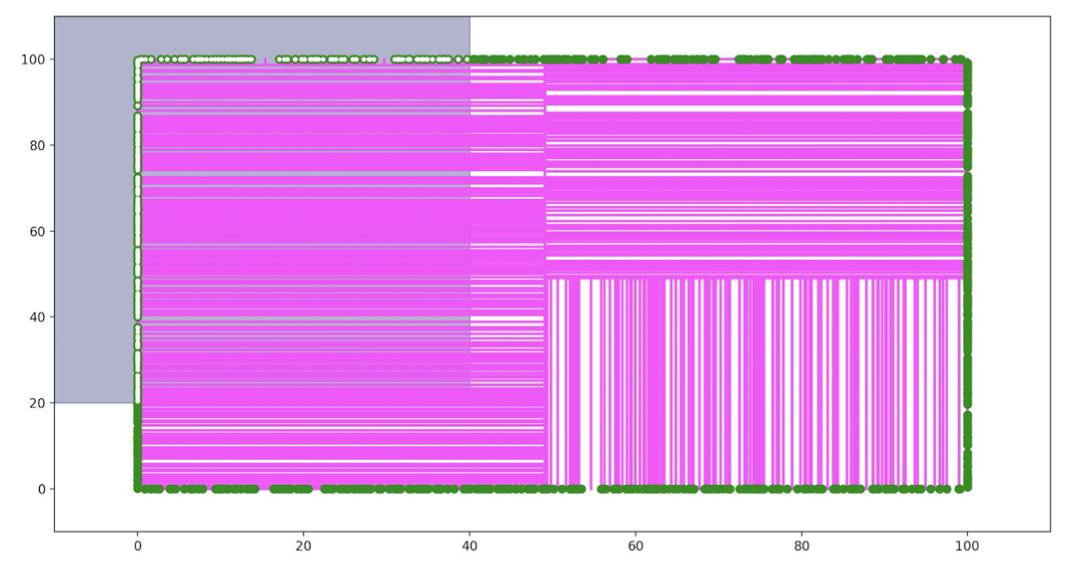
\includegraphics[width=\textwidth]{krect.png}
        \caption{Prostokąt KDTree}
      \end{figure}

      \noindent
      \quad Jak widać na zamieszczonych ilustracjach, program działa prawidłowo zarówno przy użyciu QuadTree, jak i KDTree.

      \newpage
      \begin{figure}[h!]
      \centering
        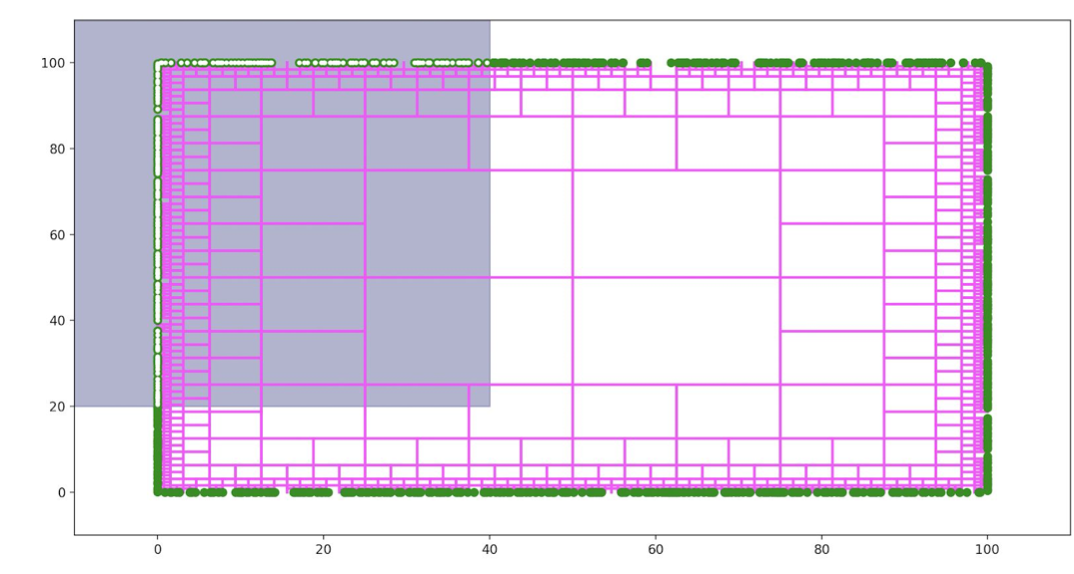
\includegraphics[width=\textwidth]{qrect.png}
        \caption{Prostokąt QuadTree}
      \end{figure}

      \noindent
      \quad Poniższa tabela i wykresy ilustrują czasy działania programów dla podanego zbioru, przy danej ilości punktów:

      \begin{table}[h!]
      \centering
      \begin{center}
      \begin{tabular}{|c|c|c|c|c|}
          \hline
          \begin{tabular}{c} Liczba \\ punktów \end{tabular} & \begin{tabular}{c} Czas \\ tworzenia \\ KDTree [s] \end{tabular} & \begin{tabular}{c} Czas \\ przeszukiwania \\ KDTree [s] \end{tabular} & \begin{tabular}{c} Czas \\ tworzenia \\ QuadTree [s] \end{tabular} & \begin{tabular}{c} Czas \\ przeszukiwania \\ QuadTree [s] \end{tabular} \\
          \hline
          500 & 0.67824 & 0.00177 & 0.75023 & 0.0011 \\
          \hline
          1000 & 2.60074 & 0.00382 & 2.69825 & 0.00134 \\
          \hline
          1500 & 5.59026 & 0.01113 & 5.86845 & 0.00158 \\
          \hline
          2000 & 9.77206 & 0.01594 & 10.14577 & 0.00186 \\
          \hline
          2500 & 15.28948 & 0.00851 & 15.5487 & 0.00177 \\
          \hline
          3000 & 21.73445 & 0.02349 & 22.24732 & 0.00182 \\
          \hline
          3500 & 31.71987 & 0.02839 & 32.46397 & 0.00231 \\
          \hline
          4000 & 43.70219 & 0.03297 & 44.47277 & 0.00269 \\
          \hline
      \end{tabular}
      \end{center}
      \caption{Wyniki pomiarów czasu dla prostokąta}
      \end{table}

      \begin{figure}[h!]
      \centering
        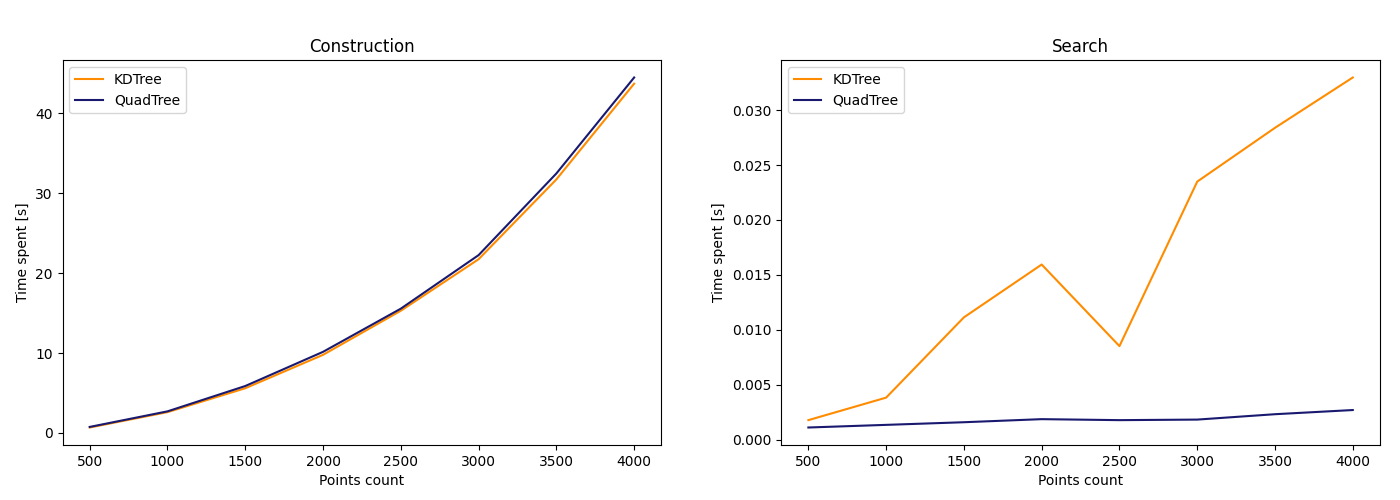
\includegraphics[width=\textwidth]{rect.png}
        \caption{Wyniki pomiarów czasu dla prostokąta}
      \end{figure}

      \noindent
      \quad Na podstawie powyższej tabeli i wykresów z następnej strony możemy stwierdzić, że dla zbioru 7 tworzenie QuadTree zajmuje średnio tyle samo czasu co KDTree . Natomiast różnica czasów przeszukiwania tych struktur zależy od ilości punktów. Dla 500 punktów przeszukiwanie KDTree działa 70\% dłużej od przeszukiwania quadtree,  dla 1500 punktów działa 7 razy dłużej, a dla 4000 punktów działa 12 razy dłużej. Oznacza to, że im bardziej konsystentnie punkty tworzą proste, tym różnica czasów jest coraz większa. Możemy, więc stwierdzić, że dla tak zadanego zbioru przeszukiwanie QuadTree działa znacznie szybciej od przeszukiwania KDTree. Możemy, więc zauważyć, biorąc pod uwagę także analizę zbioru 6, że pojawienie się punktów tworzących prostą równoległą do osi OX lub OY powoduje znaczne spowolnienie działania przeszukiwania KDTree, więc możemy stwierdzić, że dla takiego typu zbiorów należy zdecydowanie korzystać ze struktury QuadTree nad KDTree.

    \section{Testowanie dla różnych wartości \textit{capacity}}
      \quad Przeanalizowane zostanie działanie programu dla zbioru 2, dla 1000 punktów, przy różnym capacity. W szczególności przyjrzymy się poprawności oraz czasowi działania programu. 

      \noindent
      \quad Poniższe ilustracje demonstrują działanie programu przy różnych capacity:

      \begin{figure}[h!]
      \centering
        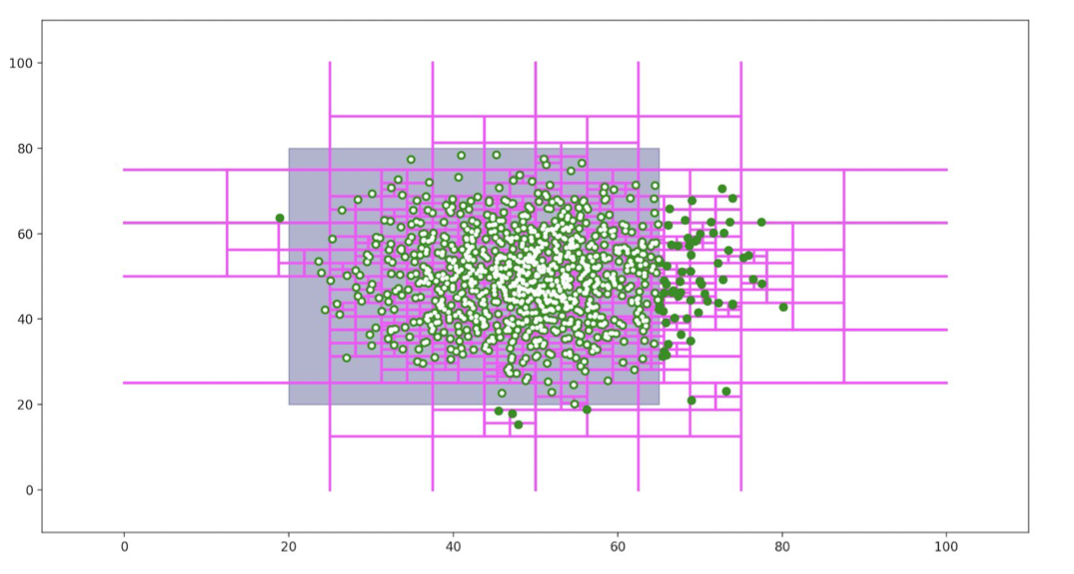
\includegraphics[width=0.63\textwidth]{qcapacity1.png}
        \caption{QuadTree : $capacity=1$}
      \end{figure}

      \begin{figure}[h!]
      \centering
        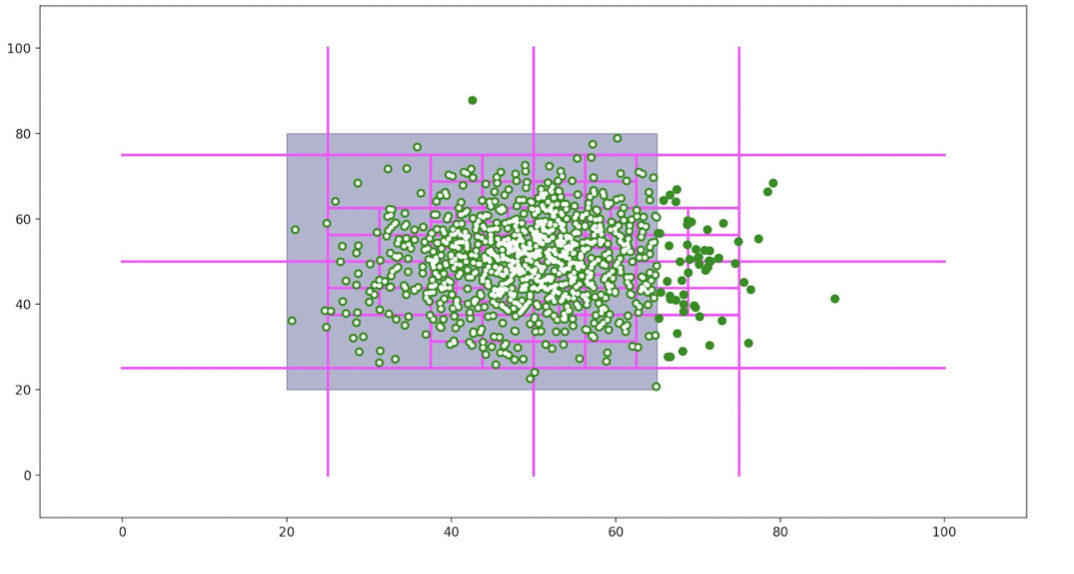
\includegraphics[width=0.63\textwidth]{qcapacity10.png}
        \caption{QuadTree : $capacity=10$}
      \end{figure}

      \begin{figure}[h!]
      \centering
        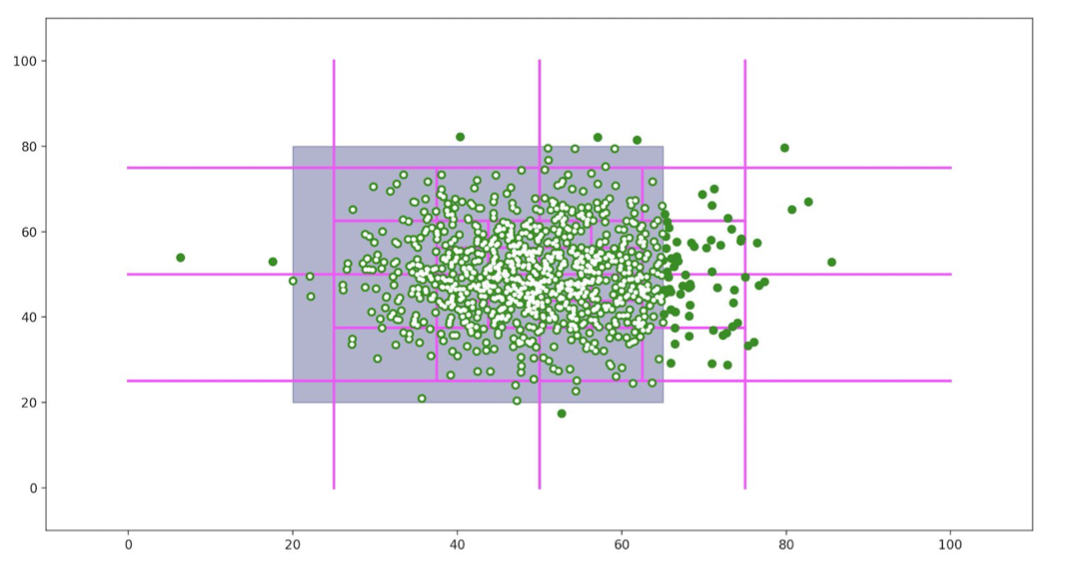
\includegraphics[width=0.66\textwidth]{qcapacity100.png}
        \caption{QuadTree : $capacity=100$}
      \end{figure}

      \begin{figure}[h!]
      \centering
        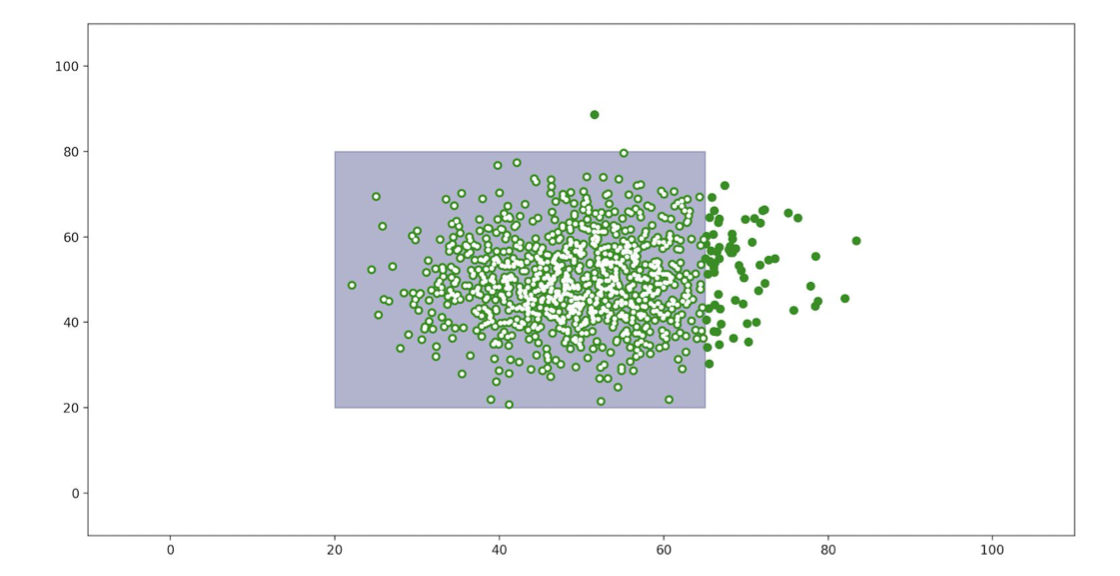
\includegraphics[width=0.71\textwidth]{qcapacity1000.png}
        \caption{QuadTree : $capacity=1000$}
      \end{figure}

      \noindent
      \quad Na podstawie powyższych ilustracji możemy stwierdzić, że program działa prawidłowo również dla capacity większym niż 1.

      \noindent
      \quad Poniższa tabela przedstawia czas konstrukcji i przeszukiwania QuadTree dla różnych capacity, dla zbioru 2:

      \begin{table}[h!]
      \centering
      \begin{center}
      \begin{tabular}{|c|c|c|}
          \hline
          Capacity & Czas konstrukcji QuadTree [s] & Czas przeszukiwania QuadTree [s] \\
          \hline
          1 & 2.90348 & 0.00475 \\
          \hline
          5 & 2.48504 & 0.00263 \\
          \hline
          10 & 2.49417 & 0.00251 \\
          \hline
          50 & 2.47602 & 0.00235 \\
          \hline
          100 & 2.46502 & 0.00242 \\
          \hline
          250 & 2.43592 & 0.00658 \\
          \hline
          500 & 2.41363 & 0.0115 \\
          \hline
          1000 & 2.38961 & 0.01142 \\
          \hline
      \end{tabular}
      \end{center}
      \caption{Wyniki pomiarów czasu dla różnych wartości $capacity$ dla QuadTree}
      \end{table}

      \begin{figure}[h!]
      \centering
        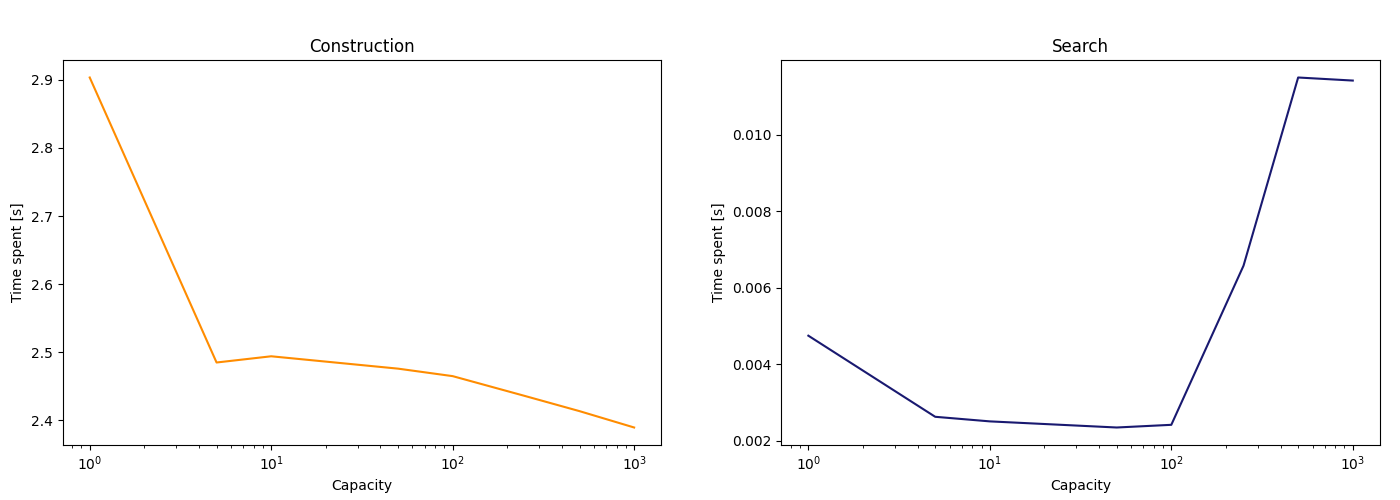
\includegraphics[width=0.93\textwidth]{capacity.png}
        \caption{Wyniki pomiarów czasu dla różnych wartości $capacity$ dla QuadTree}
      \end{figure}

      \noindent
      \quad Zauważmy, że tworzenie QuadTree jest najdłuższe dla capacity = 1, a dla reszty badanych capacity czas konstrukcji mieści się w przedziale 2.38-2.49 s. Możemy, więc powiedzieć, że wybór capacity nie wpływa znacząco na czas konstrukcji QuadTree. Czas przeszukiwania jest najkrótszy dla capacity = 50 (wśród badanych), jednakże dla capacity 5-100 jest on bardzo zbliżony.  Dla capacity większego od 100 czas przeszukiwania zbliża się do liniowego, dla capacity 1000 mamy po prostu poszukiwanie liniowe, możemy na tym przykładzie zobaczyć jego kosztowność i różnice pomiędzy capacity 1, z którego korzystaliśmy, a takze capacity 50, które jest najbardziej optymalne wśród badanych capacity. Przeszukiwanie liniowe działa 2.5-krotnie dłużej niż przy capacity 1 i 5 razy dłużej niż przy capacity 50. Udowadnia to optymalność i prawidłowość działania naszego programu (osiągamy oczekiwaną złożoność czasową, lepszą niż liniowa).

  \section{Testowanie dla różnej ilości wymiarów}
    \quad Struktura KDTree zapewnia możliwość przechowywania punktów dla różnych wymiarów. Stąd właśnie i pochodzi nazwa - KD od 'k dimensions'. Chcieliśmy zobaczyć jak zmienia się wydajność tej struktury dla różnej ilości wymiarów. Warto zauważyć, że zgodnie z teorią jest sens używania tej struktury, gdy $n >> 2^k$, gdzie $n$ - liczba punktów, $k$ - liczba wymiarów. Przetestowaliśmy dla ilości wymiarów w zakresie $[1, 50]$. O ile testowana ilość punktów jest równa 1000, to już dla $k >= 10$ - $2^k$ staje się większym od $n$, co już całkiem nie spełnia założeń dla wydajnego stosowania.

    \noindent
    \quad O ile ilość wyników jest bardzo duża, to przedstawiamy tylko wykresy:

    \begin{figure}[h!]
    \centering
      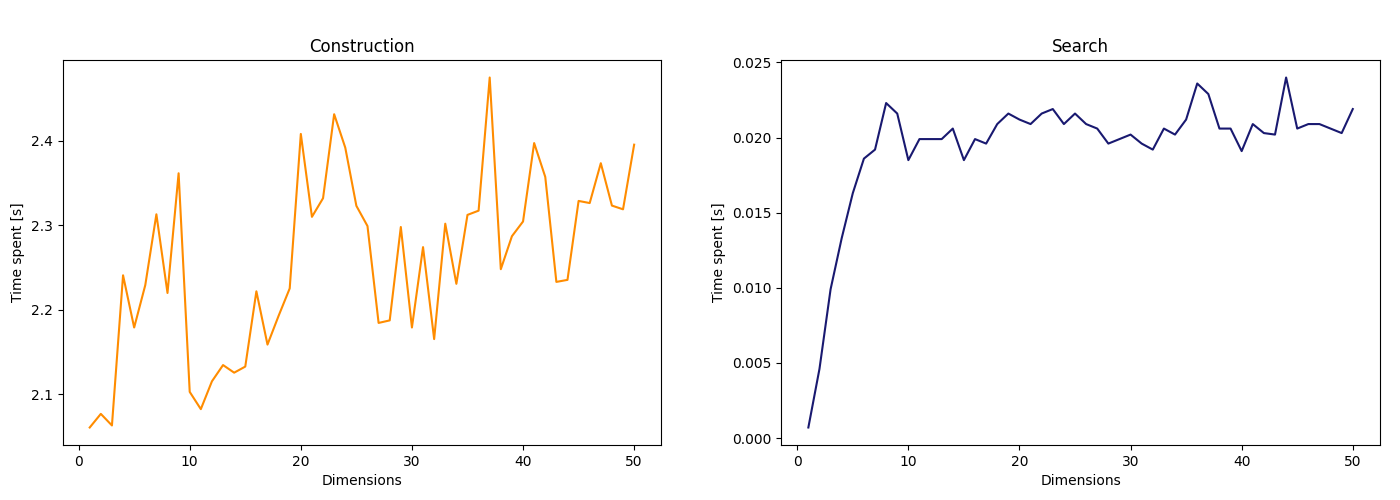
\includegraphics[width=0.93\textwidth]{dimensions.png}
      \caption{Czas budowania i przeszukiwania KDTree dla różnej ilości wymiarów}
    \end{figure}

    \noindent
    \quad Jak widzimy z wykresów, dla $k >= 10$ wydajność przeszukiwania jest bardzo niewydajna, co właśnie i stwierdziliśmy wcześniej. Dla $k \in [1, 10]$ czas gwałtownie rośnie. Czyli widzimy, że ilość wymiarów wpływa wprost na czas przeszukiwania. I dla małej ilości punktów przy dużej ilości wymiarów nie warto używać struktury KDTree.

    \noindent
    \quad Co do budowania, to możemy stwierdzić, że jest bardzo niestabilne, chociaż przedstawione wykresy są narysowane na podstawie uśrednionych wyników z trzech pomiarów. Problemem jest oczywiście losowość punktów co może powodować sytuacje gdy KDTree nie zachowuje się najlepszym sposobem (takie jak proste linie i tp). Da się stwierdzić, że istnieje tendencja do zwiększenia czasu konstruowania. Jest ona w większości spowodowana szukaniem najlepszego wymiaru dla podziału co jest $O(kn)$. To staje się dominującym czynnikiem przy konstruowaniu. Jest ono więc $O(knlogn)$. Dałoby się stworzyć $O(nlogn)$ zmieniając wymiary po kolei, ale powodowałoby to gorszą strukturę drzewa, co wpływa wprost na czas przeszukiwania. Więc uznaliśmy, że warto posłużyć się dłuższym konstruowaniem, które jest jednorazowe, żeby ulepszyć wyniki częstych operacji (podobnie jak działa język Julia, długa kompilacja i dużo optymalizacji powoduje, że sam skompilowany kod jest bardzo wydajny).

  \section{Wnioski}
    \quad Na podstawie testów przeprowadzonych dla wyżej przeanalizowanych zbiorów, możemy stwierdzić, że programy przez nas zaimplementowane działają prawidłowo i poprawnie wyznaczają podzbiór punktów należących do zadanej płaszczyzny. Dla każdego z testowanych przypadków, czas konstruowania struktur był podobny (odpowiednio dla danej liczby punktów), jest to kolejnym argumentem poświadczającym o poprawności działania zaimplementowanych  struktur. Analiza badanych zbiorów pozwala nam stwierdzić, że dla punktów rozmieszczonych równomiernie na płaszczyźnie(zbiór 1 i 3) najrozsądniej wykorzystać strukturę KDTree. Dla punktów pogrupowanych w kilka skupisk, oraz tych tworzących rozkład normalny (zbiór 2 i 4) optymalniej jest użyć struktury QuadTree. Dla zbiorów złożonych z gęstego skupiska punktów i paru punktów nie należących do tego skupiska, o tym, która struktura jest bardziej wydajna, decyduje ilość punktów należących do tego zbioru (zbiory 5.1 i 5.2). Natomiast dla zbiorów złożonych z punktów należących do prostych równoległych do osi OX lub OY (zbiór 6 i 7) należy koniecznie skorzystać ze struktury QuadTree, gdyż znacznie przyspiesza to działanie programu w porównaniu do KDTree. Przetestowanie programu dla różnych wartości capacity udowadnia, że zaimplementowane przez nas struktury osiągają złożoność lepszą od liniowej, co pozwala nam przypuszczać, że nasze programy osiągnęły złożoność oczekiwaną. 

\end{document}
% ź


